%DOCUMENTCLASS 
%
% Team 4717 2017-2018
%
\documentclass[
letterpaper, % Stock and paper size. 
11pt, % Type size.
% article,
% oneside, 
onecolumn, % Only one column of text on a page.
% openright, % Each chapter will start on a recto page.
% openleft, % Each chapter will start on a verso page.
openany, % A chapter may start on either a recto or verso page.
%draft  % Don't render images
]{article} 

%%% PACKAGES 
%%%----------------------------------------------------
\usepackage[utf8]{inputenc} % If utf8 encoding
\usepackage[T1]{fontenc}    %
\usepackage[english]{babel} % English please
\usepackage{lipsum} % generates fake test (testing)
%\usepackage[final]{microtype} % Less badboxes
\usepackage{blindtext}
%\usepackage{showframe}
%\usepackage{kpfonts} %Font
\usepackage{amsmath,amssymb,mathtools} % Math
%\usepackage[table,xcdraw]{xcolor} %for chart
\usepackage{tikz} % Figures
\usepackage{multicol}
%\usetikzlibrary{trees}
\usepackage{graphicx} % Include figures  NOTE: include [demo] to see black boxes
%\setkeys{Gin}{quiet}
%\setkeys{Gin}{keepaspectratio,width=2in,height=2in}
%\usepackage[margin=10pt,font=small,labelfont=bf,justification=raggedright]{caption}
%\usepackage{subcaption}  // memior already has it
%\usepackage{subfigure}
\usepackage{pgfplots}
\pgfplotsset{compat=1.14}
%\pgfplotsset{}
\usepackage{wrapfig}
\usepackage{soul}
\usepackage{pagenote}
\usepackage{array}
\usepackage{listings}
%\usepackage[export]{adjustbox}
%\usepackage[breaklinks]{hyperref}
\usepackage{placeins}
\usepackage[tikz]{bclogo}
\usepackage{algorithm}
\usepackage{algorithmic}

\usepackage{fancyvrb}

\usepackage[font=scriptsize]{caption}

\usepackage{tikz}
\usetikzlibrary{shapes,arrows,positioning}
\usepackage{geometry}
    \geometry{
    left=0.15\paperwidth,
    right=0.15\paperwidth,
    top=0.1\paperwidth,
    bottom=0.1\paperwidth
    }

\usepackage[pagestyles]{titlesec}

%\usepackage[right=3.5in,showframe]{geometry}

%\usepackage{hyperref} %breaks everything.  Need to look into it.
\def\hhsurl#1{\expandafter\string\csname #1\endcsname}

%Get rid of anoying pdf message about version 1.5
%\pdfminorversion=6

%The "booktabs" package makes nice tables. Sparing use of lines makes tables look much nicer (less "grid" like). %Multirow lets you make elements that span multiple rows or columns. The the package docs for examples.
%\usepackage{booktabs}
%\usepackage{multirow}

\errorcontextlines 10000
% Use \raggedbottom to stop latex from trying to add space 
% between sections to try to fill the page with text up to the 
% bottom
\raggedbottom

% \makeatletter
% % define a user command to choose the image
% % this command also creates an internal command to insert the image
% \def\@partimage{}
% \newcommand{\partimage}[2][]{\gdef\@partimage{\includegraphics[#1]{#2}}}
% \renewcommand{\printparttitle}[1]{\parttitlefont #1\vfil\@partimage\vfil}
% \makeatother

%%% PAGE LAYOUT 
%%%----------------------------------------------------

%\setlrmarginsandblock{0.15\paperwidth}{*}{1} % Left and right margin
%\setulmarginsandblock{0.1\paperwidth}{*}{1}  % Upper and lower margin
%\checkandfixthelayout

%\setbinding{4mm}
%\settypeblocksize{*}{24.5pc}{1.618}
%\setlrmargins{*}{*}{1.5}
%\setulmarginsandblock{6pc}{7pc}{*}
%\setmarginnotes{6pt}{6pc}{12pt}
%\strictpagecheck
%\setlength{\topskip}{1.6\topskip}
%\checkandfixthelayout

%%% SECTIONAL DIVISIONS
%%%----------------------------------------------------

%%%%%%%%%%%%%%%%%%%%%%%%%%%%%%%%%%%%%%%%%%%%%%%
% reset chapter numbers on each part
%
\makeatletter
\@addtoreset{chapter}{part}
\makeatother

%%%%%%%%%%%%%%%%%%%%%%%%%%%%%%%%%%%%%%%%%%%%%%%
% Part: center title
%
\titleformat{\part}[display]
{\normalfont\LARGE\color{blue}\bfseries\centering}{}{0pt}{}
[{\titlerule[0.8pt]}]

%%%%%%%%%%%%%%%%%%%%%%%%%%%%%%%%%%%%%%%%%%%%%%%
% SubSection: center title
%
% \titleformat{\subsection}[display]
% {\normalfont\LARGE\color{blue}\bfseries\centering}{}{0pt}{}

%%%%%%%%%%%%%%%%%%%%%%%%%%%%%%%%%%%%%%%%%%%%%%%
% Remove section headers
%
\makeatletter
\titleformat{\section}[runin]{}{}{0pt}{\@gobble}
\titleformat{\subsection}[runin]{}{}{0pt}{\@gobble}
\makeatother
\titlespacing{\section}{\parindent}{0pt}{0pt}
\titlespacing{\subsection}{\parindent}{0pt}{0pt}


%\maxsecnumdepth{subsection} % Subsections (and higher) are numbered
%\setsecnumdepth{subsection}


%\setsecheadstyle{\normalfont\large\bfseries}
%\setsubsecheadstyle{\normalfont\normalsize\bfseries}
%\setparaheadstyle{\normalfont\normalsize\bfseries}
%\setparaindent{0pt}\setafterparaskip{0pt}

%%% FLOATS AND CAPTIONS
%%%----------------------------------------------------

\makeatletter                  % You do not need to write [htpb] all the time
\renewcommand\fps@figure{htbp} %
\renewcommand\fps@table{htbp}  %
\makeatother                   %

%\captiondelim{\null\newline}
%\captionnamefont{\small\sffamily\bfseries}
%\captiontitlefont{\small\sffamily\linespread{.84}\selectfont}
%\captionstyle[\centering]{\raggedright}
%\normalcaptionwidth
%\captiontitlefinal{.}
%\setlength\belowcaptionskip{.5ex}

%\changecaptionwidth          % Change the width of the caption
%\captionwidth{1\textwidth} %

%%% ABSTRACT
%%%----------------------------------------------------

%\renewcommand{\abstractnamefont}{\normalfont\small\bfseries} % Font of abstract title
%\setlength{\absleftindent}{0.1\textwidth} % Width of abstract
%\setlength{\absrightindent}{\absleftindent}

%%% HEADER AND FOOTER 
%%%----------------------------------------------------


%
% Add graphics directories to search
%
%\graphicspath{{Images/}}

%%% TABLE OF CONTENTS
%%%----------------------------------------------------

% Only parts, chapters and sections in the table of contents
%\maxtocdepth{subsection} 
%\settocdepth{subsection}

% Make overflow at end of line for big pages numbers go away
%\setpnumwidth{2.5em}

% Center part number on line and add color
%\makeatletter
%\renewcommand{\partnumberline}[1]{\sffamily\large\bfseries\color{blue}\hfil\hspace\@tocrmarg Part #1:~}
%\makeatother
%\renewcommand{\cftpartfont}{\large\normalfont}
%\cftpagenumbersoff{part}

% Add Colored text before each "part" of TOC
%\cftpagenumbersoff{part}
%\renewcommand{\cftpartpresnum}{\sffamily\large\bfseries\color{blue}\partname\ }
%\renewcommand{\cftpartaftersnumb}{\\}
%\cftsetindents{part}{0em}{0em}

% Center Part Numbers in TOC
%\makeatletter
%\renewcommand\partnumberline[1]{\hfil\hspace\@tocrmarg #1~}
%\makeatother

% Add a \par to the end of the TOC
\AtEndDocument{\addtocontents{toc}{\par}} 

% Add "Meeting" at the start of each TOC entry
%\renewcommand{\cftchaptername}{Meeting\space}

%%% INTERNAL HYPERLINKS
%%%----------------------------------------------------

%\usepackage{hyperref}   % Internal hyperlinks
%\hypersetup{
%pdfborder={0 0 0},      % No borders around internal hyperlinks
%pdfauthor={I am the Author} % author
%}
%\usepackage{memhfixc}

%%% NEW COMMANDS
%%%----------------------------------------------------
\usepackage{wrapfig}
\usepackage{calc}
\usepackage{adjustbox}
\usepackage{graphicx}
\usepackage{float}

\newcommand{\insertbio}[7]{
	\newpage	
	\pagestyle{hhsstyle}
	\begin{flushright}
	\textbf{\Huge #1}
	\end{flushright}
	%\addcontentsline{toc}{section}{\numberline{}#1}
	\section{#1}
    %\index{#1} 
	%\newlength{\strutheight}
	%\settoheight{\strutheight}{\strut}
	\begin{adjustbox}{valign=T,
    				%raise=\strutheight,
                    minipage={\linewidth}}
    	\begin{wrapfigure}{R}{0pt}
    		% Portrait shot: looks best in 2:3 ratio, square is acceptable
            \includegraphics[width=6cm,height=5cm,keepaspectratio, angle = 270]{Bios/Images/#2} 
            %\includegraphics[width=6cm,height=5cm,angle = 270]{Bios/Images/#2} 
    	\end{wrapfigure}
    	\strut{}
    \end{adjustbox}
    \subsection*{Quick Facts}
	\begin{itemize}
		\item \textsc{\large Interests:} #3
		\item \textsc{\large Sub-Team:} #4
		\item \textsc{\large Year:} #5
	\end{itemize}
	\vspace{1cm}		
	\subsection*{Biography}
	#6	
	\begin{figure}[H]
	\centering
	\begin{minipage}{.5\textwidth}
	  \centering
	  \includegraphics[width=0.95\linewidth]{Bios/Images/#7}
	  %\captionof{figure}{Figure 1}
	  %\label{fig:test1}
	\end{minipage}%
	\end{figure}
}



\usepackage{wrapfig}
\usepackage{calc}
\usepackage{adjustbox}
\usepackage{graphicx}
\usepackage{float}

\newcommand{\insertbiomentor}[6]{
	%\newpage	
	\section{#1}
	%\pagestyle{plain}
	\begin{flushright}
	\textbf{\Huge #1}
	\end{flushright}
	%\addcontentsline{toc}{section}{\numberline{}#1}
    %\index{#1} 
	%\newlength{\strutheight}
	%\settoheight{\strutheight}{\strut}
	\begin{adjustbox}{valign=T,
    				%raise=\strutheight,
                    minipage={\linewidth}}
    	\begin{wrapfigure}{R}{0pt}
    		%\includegraphics[width=160px]{Bios/#2} 
            \includegraphics[width=7cm,height=7cm,keepaspectratio]{Bios/Images/#2} 
            % Portrait shot: looks best in 2:3 ratio, square is acceptable
    	\end{wrapfigure}
    	\strut{}
    \end{adjustbox}
    \subsection*{Quick Facts}
	\begin{itemize}
		\item \textsc{\large Occupation:} #3
		\item \textsc{\large Relation to Team:} #4
        \item \textsc{\large Interests:} #5
	\end{itemize}
	\vspace{3cm}		
	\subsection*{Biography}
	#6	
}

\newcommand{\insertCV}[7]{

\flushleft

\begin{quotebox}
\textsl{\Huge #2} \\
\flushright{\textrm{\large{\textbf{- #3}}}}
\end{quotebox}

\raggedright
\vskip 0.2in
\textbf{\huge #1}
\vskip 0.1in

\begin{figure}[h!]
\centering
\begin{minipage}{.48\textwidth}
  \centering
  \includegraphics[width= .8\linewidth]{Core_Values/#6}
\end{minipage}%
\hfill
\begin{minipage}{.48\textwidth}
  \centering
  \includegraphics[width= .8\linewidth]{Core_Values/#7}
\end{minipage}
\end{figure}

\begin{centering}
#4
\end{centering}
\vskip 0.2in
Refer to these pages to see more of this Core Value:
\vskip 0.2in
\begin{itemize}
#5 %use \item[$\blacksquare$]
\end{itemize}
}
\usepackage{wrapfig}
\usepackage{calc}
\usepackage{adjustbox}
\usepackage{graphicx}
\usepackage{float}

\newcommand{\insertOutreachEvent}[8]{
	\newpage	
	\pagestyle{plain}
	{
	\setthemecolor[DmgLilac]
	\begin{commentbox}{\flushleft{\huge{{\textrm{#1}}}}}
\flushleft
\textrm{\textbf{Date:} #2} \\
\textrm{\textbf{Event Total:} #3 Hours} \\
	\end{commentbox}
	}
	
	\addcontentsline{toc}{section}{\numberline{}#1}

	{
    \noindent\makebox[\textwidth][c]{%
	\begin{minipage}{\textwidth}
	  \centering
	  \includegraphics[width=0.75\linewidth]{Outreach/Images/#4}
	  %\captionof{figure}{Figure 1}
	  %\label{fig:test1}
	\end{minipage}}%
    }
    
    \setthemecolor[DmgLavender]	
    \begin{paperbox}{\flushleft{{Purpose:}}}
    
    \flushleft{#5}
    
    \end{paperbox}
    
    {\flushleft{\textbf{Description:}}} \\*

	#6	
	% \begin{figure}[H]
	% \centering
	% \begin{minipage}{.5\textwidth}
	%   \centering
	%   \includegraphics[width=0.9\linewidth]{Outreach/Images/#7}
	%   %\captionof{figure}{Figure 1}
	%   %\label{fig:test1}
	% \end{minipage}%
	% \begin{minipage}{.5\textwidth}
	%   \centering
	%   \includegraphics[width=0.9\linewidth]{Outreach/Images/#8}
	%   %\captionof{figure}{Figure 2}
	%   %\label{fig:test2}
	% \end{minipage}
	% \end{figure}

 \begin{figure}[h!]
 \centering
   \includegraphics[width=\textwidth, angle=0]{Outreach/Images/#7}
 \end{figure}

 \begin{figure}[h!]
 \centering
   \includegraphics[width=\textwidth, angle=0]{Outreach/Images/#8}
 \end{figure}
}
%%%%%%%%%%%%%%%%%%%%%%%%%%%%%%%%%%%%%%%%%%%%%%
%             insertCompetition
% 1) Competition Name (ex. Ruckus at the Rock)
% 2) Date (MM/DD/YYYY)
% 3) Location (ex. Hagerty High School)
% 4) Meet Ranking (ex. 5th)
% 5) Match Results Breakdown (image file path)
% 6) Match Scoring Pie Chart (image file path)
% 7) Competition OPR Breakdown (image file path)
% 8) Reflection (text)
%%%%%%%%%%%%%%%%%%%%%%%%%%%%%%%%%%%%%%%%%%%%%%

\usepackage{wrapfig}
\usepackage{calc}
\usepackage{adjustbox}
\usepackage{graphicx}
\usepackage{float}

\newcommand{\insertCompetition}[8]{
	\newpage	
	\pagestyle{plain}
	%\begin{flushleft}
    \begin{description}
		\item [\Huge Competition:] {\Huge #1}
		\item [Date:] #2
		\item [Location:] #3
        \item [Meet Ranking: #4]
	\end{description} 
	\addcontentsline{toc}{section}{\numberline C#1 Competition: #2}

	\begin{figure}[h!]
    \centering
    \includegraphics[width=0.8\textwidth, angle=0]{Competition/Images/#5}
    \end{figure}
    
    \begin{figure}[h!]
	\centering
	\begin{minipage}{.5\textwidth}
	  \centering
	  \includegraphics[width=0.95\linewidth]{Competition/Images/#6}
	\end{minipage}%
	\begin{minipage}{.5\textwidth}
	  \centering
	  \includegraphics[width=0.95\linewidth]{Competition/Images/#7}
	\end{minipage}
	\end{figure}
    
	\subsection*{What happened:}
    {#8}
    
 }

%%%%%%%%%%%%%%%%%%%%%%%%%%%%%%%%%%%%%%%%%%%%%%
%                insertmeeting
% 1) Title (something creative & funny?)
% 2) Date (MM/DD/YYYY)
% 3) Location (ex. Hagerty High School)
% 4) People/Committees Present 
% 5) Picture 
% 6) Start Time & Stop Time (ex. 12:30AM to 4:30PM)
%%%%%%%%%%%%%%%%%%%%%%%%%%%%%%%%%%%%%%%%%%%%%%

\newcommand{\insertmeeting}[7]{
% pagestyle
%   meeting - chapter and section on the same heading
%   headings - 
%   ruled - horizontal line in the heading
\section*{#1}
\pagestyle{hhsstyle}
\addcontentsline{toc}{section}{\numberline{}#2 - #1}
% \section[#2 - #1]{#2}
% \chapter[#2 - #1]{#2}
% \index{#2} 

\begin{figure}[h]
\begin{minipage}[b]{0.6\linewidth}
    \begin{description}
        \item [\Large \textcolor{black}{#1}]
        \item #2
        \item #3
        \item #4
        \item #6
    \end{description} 
\end{minipage}%
\hfill
\begin{minipage}[b]{0.35\linewidth}
	\raggedleft

    %\includegraphics[scale=0.3]{#5}
    %\setlength{\fboxsep}{0pt}\fbox{
    %\includegraphics[width=.3\linewidth]
    %\frame{\includegraphics[width=3cm,height=3cm,keepaspectratio]
    \fbox{\includegraphics[width=3cm,height=3cm,keepaspectratio]
    {#5}}
    \centering
    \par Robot
\end{minipage}
%\noindent\rule{\textwidth}{1pt}
\vspace{5mm}
\begingroup % because of color
	\color{gray}%
	\hrule width \hsize \kern 1mm \hrule width \hsize height 2pt 
\endgroup

\end{figure}%
}  %end newcommand

%%%%%%%%%%%%%%%%%%%%%%%%%%%%%%%%%%%%%%%%%%%%%%
%                newsection
%
% 1) Committee/Subcommittee Name (ex. Hardware & Design)
% 2) List of Goals (remember to use \item)
% 3) Accomplishments (written in third person collective)
%%%%%%%%%%%%%%%%%%%%%%%%%%%%%%%%%%%%%%%%%%%%%%

\newcommand{\newsection}[4]{
\addcontentsline{toc}{subsection}{\numberline{}#1}

\subsection*{#1}
\noindent\hfil\rule{\textwidth}{.4pt}\hfil
\begin{multicols}{2}

\setthemecolor[PhbLightGreen]

\begin{paperbox}{\flushleft{Goals:}}

{
\flushleft
\begin{itemize}
#2
\end{itemize}
}

\end{paperbox}

{\flushleft{\textbf{\large ACCOMPLISHMENTS:}}} \\*
\vspace{2mm}
#3

\end{multicols}


{

\setthemecolor[DmgLilac]
\begin{paperbox}[float=!h]{\flushleft{Next on the Docket:}}
\flushleft{#4}
\end{paperbox}

}

}  %end newcommand

%%%%%%%%%%%%%%%%%%%%%%%%%%%%%%%%%%%%%%%%%%%%%%
%                insertimage
%
% 1) Image File Path 
% 2) Caption (Camel Case, Short & Descriptive)
% 3) Label (UNIQUE identifier for each image)
%%%%%%%%%%%%%%%%%%%%%%%%%%%%%%%%%%%%%%%%%%%%%%

\newcommand{\insertmeetingimage}[3]{

\begin{wrapfigure}{c}{0.75\linewidth}
\includegraphics[width=\linewidth]{#1}
\caption{#2}
\label{fig:#3}
\end{wrapfigure}

}
%This allows the meeting chapters to show up on the toc but not have a header page :)

\makeatletter
\newcommand{\unchapter}[1]{%
  \begingroup
  \let\@makechapterhead\@gobble % make \@makechapterhead do nothing
  \chapter{#1}
  \endgroup
}
\makeatother
\usepackage{wrapfig}
\usepackage{calc}
\usepackage{adjustbox}
\usepackage{graphicx}
\usepackage{float}

\newcommand{\insertdesignoverview}[6]{
	\newpage	
	\pagestyle{plain}
	\begin{flushright}
	\textbf{\Huge #1}
	\end{flushright}
	\addcontentsline{toc}{section}{\numberline{}#1}
    %\index{#1} 
	%\newlength{\strutheight}
	%\settoheight{\strutheight}{\strut}
   
 %\vspace{.25cm}		
	\subsection*{Goal: \hl{#2}}

   \begin{figure}[H]
	\centering
	\begin{minipage}{.5\textwidth}
	  \centering
	  \includegraphics[width=0.95\linewidth]{Design_Overview/#3}
	  %\captionof{figure}{Figure 1}
	  %\label{fig:test1}
	\end{minipage}%
	\begin{minipage}{.5\textwidth}
	  \centering
	  \includegraphics[width=0.95\linewidth]{Design_Overview/#4}
	  %\captionof{figure}{Figure 2}
	  %\label{fig:test2}
	\end{minipage}
	\end{figure}
    
%	\vspace{.25cm}		
	\subsection*{Core Materials}
	#5

%	\vspace{.25cm}		
	\subsection*{Manufacturing Processes}
	#6
	\vspace{.1cm}


	
%	\vspace{.25cm}		
%	\subsection*{Description}

}
\usepackage{adjustbox}

%%%%%%%%%%%%%%%%%%%%%%%%%%%%%%%%%%%%%%%%%%%%%%%%%%
% 1 Name
% 2 Bio Image
% 3 Quote
% 4 Committees
% 5 Current grade
% 6 Leave Blank
% 7 Stats, with & between each stat
%%%%%%%%%%%%%%%%%%%%%%%%%%%%%%%%%%%%%%%%%%%%%%%%%%
\newcommand{\dndbio}[7]{
	\newpage
	\addcontentsline{toc}{section}{\numberline{}#1}
	\begin{figure}
	\centering
	\includegraphics[height=.45\paperwidth, keepaspectratio]{Bios/Images/#2}
	\end{figure}
	\begin{monsterboxnobg}{#1}
		\begin{hangingpar}
	    	\textit{``#3''}
	  	\end{hangingpar}
	\dndline
	\basics[%
		committees = \Large{#4},
		Current Grade = \Large{#5},
		Stats = \Large{#6}
	]
	\vspace{3mm}
	\stats[
	    STAT = \stat{#7}
	]
	\dndline%
	\end{monsterboxnobg}
}


%%%%%%%%%%%%%%%%%%%%%%%%%%%%%%%%%%%%%%%%%%%%%%%%%%
% Use \monstersection{"Title"} beforehand to create a section (which is just a list), then use this command to create entries in the list
% 1 Entry
% 2 Description
%%%%%%%%%%%%%%%%%%%%%%%%%%%%%%%%%%%%%%%%%%%%%%%%%%
\newcommand{\dndaction}[2]{
	\begin{monsteraction}[\large{#1}]
	        #2
	    \end{monsteraction}
}
\usepackage{wrapfig}


%%%%%%%%%%%%%%%%%%%%%%%%%%%%%%%%%
% 1 5-6 line introduction of current finances
% 2 Funding goals image path
% 3 Label for the funding goals
% 4 Table of funds 
% 5 Label for table
% 6 Pie Chart of breakdown
% 7 Label for pie chart
% 8 Bar chart of how we use our money
% 9 Label for the use
%%%%%%%%%%%%%%%%%%%%%%%%%%%%%%%%%
\newcommand{\financemodule}[9]{
	
	\newpage
	\addcontentsline{toc}{section}{Business Plan}
	\large{\textbf{Current Financials: }#1}\\

	% make this a lot longer, fill 4-5 lines in the pdf
	\large{Our original funding goals can be visualized through \ref{fig:#3}.}\\

	\begin{figure}[h!]
    	\centering
    	\includegraphics[width=0.6\textwidth]{#2}
		\label{fig:#3}
		\caption{Current Funding Goals}	
	\end{figure}

	\large{We receive funds through multiple sources, with \ref{fig:#5} showing the complete breakdown of our team's funding, and the source of funding is shown through \ref{fig:#7}.}\\

	\newpage
	\begin{figure}[h!]
		\begin{minipage}{.5\textwidth}
			\centering
	    	\includegraphics[width=0.98\linewidth]{#4}
			\label{fig:#5}
			\caption{The team's total funding}
		\end{minipage}%
		\begin{minipage}{.5\textwidth}
			\centering
	    	\includegraphics[width=0.98\linewidth]{#6}
			\label{fig:#7}
			\caption{A breakdown of the funding}
	\end{minipage}
	\end{figure}

	\begin{figure}[h!]
		\centering
		\includegraphics[width=.6\textwidth]{#8}
		\label{fig:#9}
		\caption{How we use our money}
	\end{figure}

	\Large{"Some comparison of how we expected to spend our money and how we actually spended our money"}
}
\newcommand{\hhscommittee}[1]{
\subsection{#1}
\begin{bclogo}[couleur=blue!30, arrondi=0.2, logo=\bccrayon]{#1 Committee}
\end{bclogo}
\noindent\hfil\rule{\textwidth}{.4pt}\hfil
}
\newcommand{\whatsnext}[1]{
\subsection*{What's Next}
\begin{bclogo}[couleur=pgrey!30, arrondi=0.2, logo=\bchorloge]{Next on the Docket} #1
\end{bclogo}
\noindent\hfil\rule{\textwidth}{.4pt}\hfil
}

%%%%%%%%%%%%%%%%%%%%%%%%%%%%%%%%%%%%%%%%%%%%%%
% new itemize enviroment that doesn't allow latex to put 
% more space between items when it tries to fill the entire 
% page with text.  If you use /raggedbottom then this is not needed.
\newenvironment{myitemize}
{ \begin{itemize}
    \setlength{\itemsep}{0pt}
    \setlength{\parskip}{0pt}
    \setlength{\parsep}{0pt}     }
{ \end{itemize}  }


%%%%%%%%%%%%%%%%%%%%%%%%%%%%%%%%%%%%%%%%%%%%%%
% Pagenote section
% Use page notes to mark control and innovation
\makepagenote
%\continuousnotenums
%\notepageref
\renewcommand*{\pagenotesubhead}[3]{}

%%%%%%%%%%%%%%%%%%%%%%%%%%%%%%%%%%%%%%%%%%%%%%
% Control label
% 
\makeatletter
\newcommand{\interesting}[2]{%
  \@bsphack
  \csname phantomsection\endcsname % in case hyperref is used
  \def\@currentlabel{#1}{\label{#2}}%
  \@esphack
}
\makeatother

%%%%%%%%%%%%%%%%%%%%%%%%%%%%%%%%%%%%%%%%%%%%%%
% Interesting Page Table
% 
\newcommand{\interestingpagetable}{
	\newpage	
	%\pagestyle{plain}
	\textbf{\Huge Interesting Pages}
	\addcontentsline{toc}{section}{\numberline{}Interesting Pages}
  
 	\vspace*{1cm}
	 %\par 
    We have created the table below that highlights some of the more interesting pages in our notebook.  The highlighted ones are also tabbed.
    
    \vspace*{1cm}
    
    % more space between rows
    \renewcommand{\arraystretch}{1.2} 
    % Remove space to the vertical edges
    %\begin{tabular}{@{}lll@{}}
    
    %\interesting{This is an example of a good control}{control:1} % enter this in the actual page file
    
\resizebox{\textwidth}{!}{%
    \begin{tabular}{lp{0.7\textwidth}r}
		\toprule
		Type & Description & Page \\ 
	\midrule
            
            Innovate & \ref{innovate:1} & \pageref{innovate:1}\\
            Innovate & \ref{innovate:3} & \pageref{innovate:3}\\
            Innovate & \ref{Innovate:4} & \pageref{Innovate:4}\\
            Innovate & \ref{Innovate:55} & \pageref{Innovate:55}\\
            Design & \ref{design:1} & \pageref{design:1}\\
            Design & \ref{design:2} & \pageref{design:2}\\
            Design & \ref{design:3} & \pageref{design:3}\\
            Design & \ref{design:5} & \pageref{design:5}\\
            Design & \ref{design:6} & \pageref{design:6}\\
            Control & \ref{control:1} & \pageref{control:1}\\
            Control & \ref{control:2} & \pageref{control:2}\\
            Control & \ref{control:3} & \pageref{control:3}\\
            Control & \ref{control:4} & \pageref{control:4}\\
            Control & \ref{innovate:2} & \pageref{innovate:2}\\
            Control & \ref{control:77} & \pageref{control:77}\\
            Control & \ref{control:44} & \pageref{control:44}\\
            Control & \ref{control:99} & \pageref{control:99}\\
            Connect & \ref{connect:1} & \pageref{connect:1}\\
            Connect & \ref{connect:2} & \pageref{connect:2}\\
            Connect & \ref{connect:3} & \pageref{connect:3}\\
            Connect & \ref{connect:4} & \pageref{connect:4}\\
            Think & \ref{timeline:1} & \pageref{timeline:1}\\
            Think & \ref{think:1} & \pageref{think:1}\\
            Think & \ref{think:2} & \pageref{think:2}\\
            Competition & \ref{competition:1} & \pageref{competition:1}\\
            Competition & \ref{competition:2} & \pageref{competition:2}\\
            Competition & \ref{competition:3} & \pageref{competition:3}\\
	
           
		\bottomrule
	\end{tabular}
}
    \vspace{.5cm}
\newline \textbf{Recent Update: We are now balancing without touching the ground with our arms!} For more information, please see the control sections.
}

\makepagenote

% %Code to make Figures stay within their \section (i.e. Programming):
% \makeatletter
%     \renewcommand\section{\@startsection {section}{1}{\z@}%
%        {-3.5ex \@plus -1ex \@minus -.2ex}%
%        {2.3ex \@plus.2ex}%
%        {\FloatBarrier\normalfont\large\bfseries}}
% \makeatother

%Code to make Figures stay within their \subsection (i.e. Accomplishments):
% \makeatletter
% \AtBeginDocument{%
%   \expandafter\renewcommand\expandafter\subsubsection\expandafter
%     {\expandafter\@fb@secFB\subsubsection}%
%   \newcommand\@fb@secFB{\FloatBarrier
%     \gdef\@fb@afterHHook{\@fb@topbarrier \gdef\@fb@afterHHook{}}}%
%   \g@addto@macro\@afterheading{\@fb@afterHHook}%
%   \gdef\@fb@afterHHook{}%
% }
% \makeatother

\makeatletter
\AtBeginDocument{%
  \expandafter\renewcommand\expandafter\subsection\expandafter
    {\expandafter\@fb@secFB\subsection}%
  \newcommand\@fb@secFB{\FloatBarrier
    \gdef\@fb@afterHHook{\@fb@topbarrier \gdef\@fb@afterHHook{}}}%
  \g@addto@macro\@afterheading{\@fb@afterHHook}%
  \gdef\@fb@afterHHook{}%
}
\makeatother

\definecolor{pblue}{rgb}{0.13,0.13,1}
\definecolor{pgreen}{rgb}{0,0.5,0}
\definecolor{pred}{rgb}{0.9,0,0}
\definecolor{pgrey}{rgb}{0.46,0.45,0.48}

\lstset{language=Java,
  showspaces=false,
  showtabs=false,
  breaklines=true,
  showstringspaces=false,
  breakatwhitespace=true,
  commentstyle=\color{pgreen},
  keywordstyle=\color{pblue},
  stringstyle=\color{pred},
  basicstyle=\ttfamily,
  moredelim=[il][\textcolor{pgrey}]{$$},
  moredelim=[is][\textcolor{pgrey}]{\%\%}{\%\%}
}


% \newpagestyle{hhsstyle}[\small]{
%   \sethead[\thepage][][\thesection~\sectiontitle]{\subsectiontitle}{}{\thepage}
% }

\newpagestyle{hhsstyle}[\small]{
\sethead[][][\thesection~\sectiontitle]{\subsectiontitle}{}{}
\setfoot[\thepage][][]{}{}{\thepage}
}



% \setlrmarginsandblock{0.15\paperwidth}{*}{1}

%\includeonly{} % Test single documents temporarily

\makepagenote



%%%%%%%%%%%%%%%%%%%%%%%%%%%%%%%%%%%%%%%%%%%%%%
%%%
%%%               THE DOCUMENT
%%%
%%%%%%%%%%%%%%%%%%%%%%%%%%%%%%%%%%%%%%%%%%%%%%

%\pretitle{\begin{center}\Huge\bfseries}
\author{Hagerty High School}
\title{4717 Mechromancers}
%\usepackage{lipsum} % Just to put in some text
\begin{document}
%\frontmatter
\maketitle

%\begin{abstract}
%\end{abstract}

\begin{figure}[ht]
	\centering
    \par\itshape
	WE BRING ROBOTS TO LIFE!!!
	\par\vskip4em
	\par\vfill
    
\includegraphics[width=	1.0\textwidth]{Images/Main/4717Logo.png}
\end{figure}

%\clearpage
\cleardoublepage

% Below can be used to create a X on a large blank space on the pages. 

% \begin{figure}[h!]
% \centering
% \includegraphics[width=0.4\textwidth, angle=90]{The_X.png}
% \end{figure}

\tableofcontents
\clearpage
%\mainmatter

 %           _______                     _____           _            
 %          |__   __|                   |  __ \         | |           
 %  ______     | | ___  __ _ _ __ ___   | |__) |_ _ _ __| |_   ______ 
 % |______|    | |/ _ \/ _` | '_ ` _ \  |  ___/ _` | '__| __| |______|
 %             | |  __/ (_| | | | | | | | |  | (_| | |  | |_          
 %             |_|\___|\__,_|_| |_| |_| |_|   \__,_|_|   \__|         
                                                                                                                                    
\part{Team Section}
\begin{minipage}[c]{\linewidth}
\centering
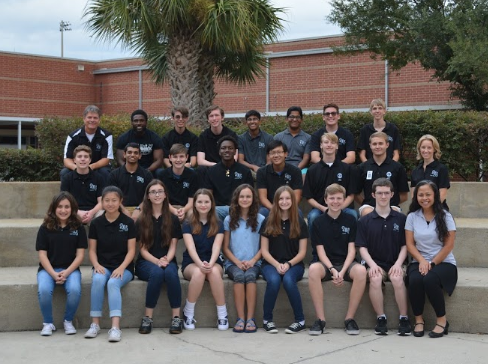
\includegraphics[width=\linewidth]{Images/Team/Team_Main.PNG}
\end{minipage}

\cleardoublepage

% \noindent
% \textbf{\Huge Summary}
% \newline
% \pagestyle{plain}
% \addcontentsline{toc}{section}{\numberline{}Summary}
% %\begin{figure}[ht]
% %\centering
% %  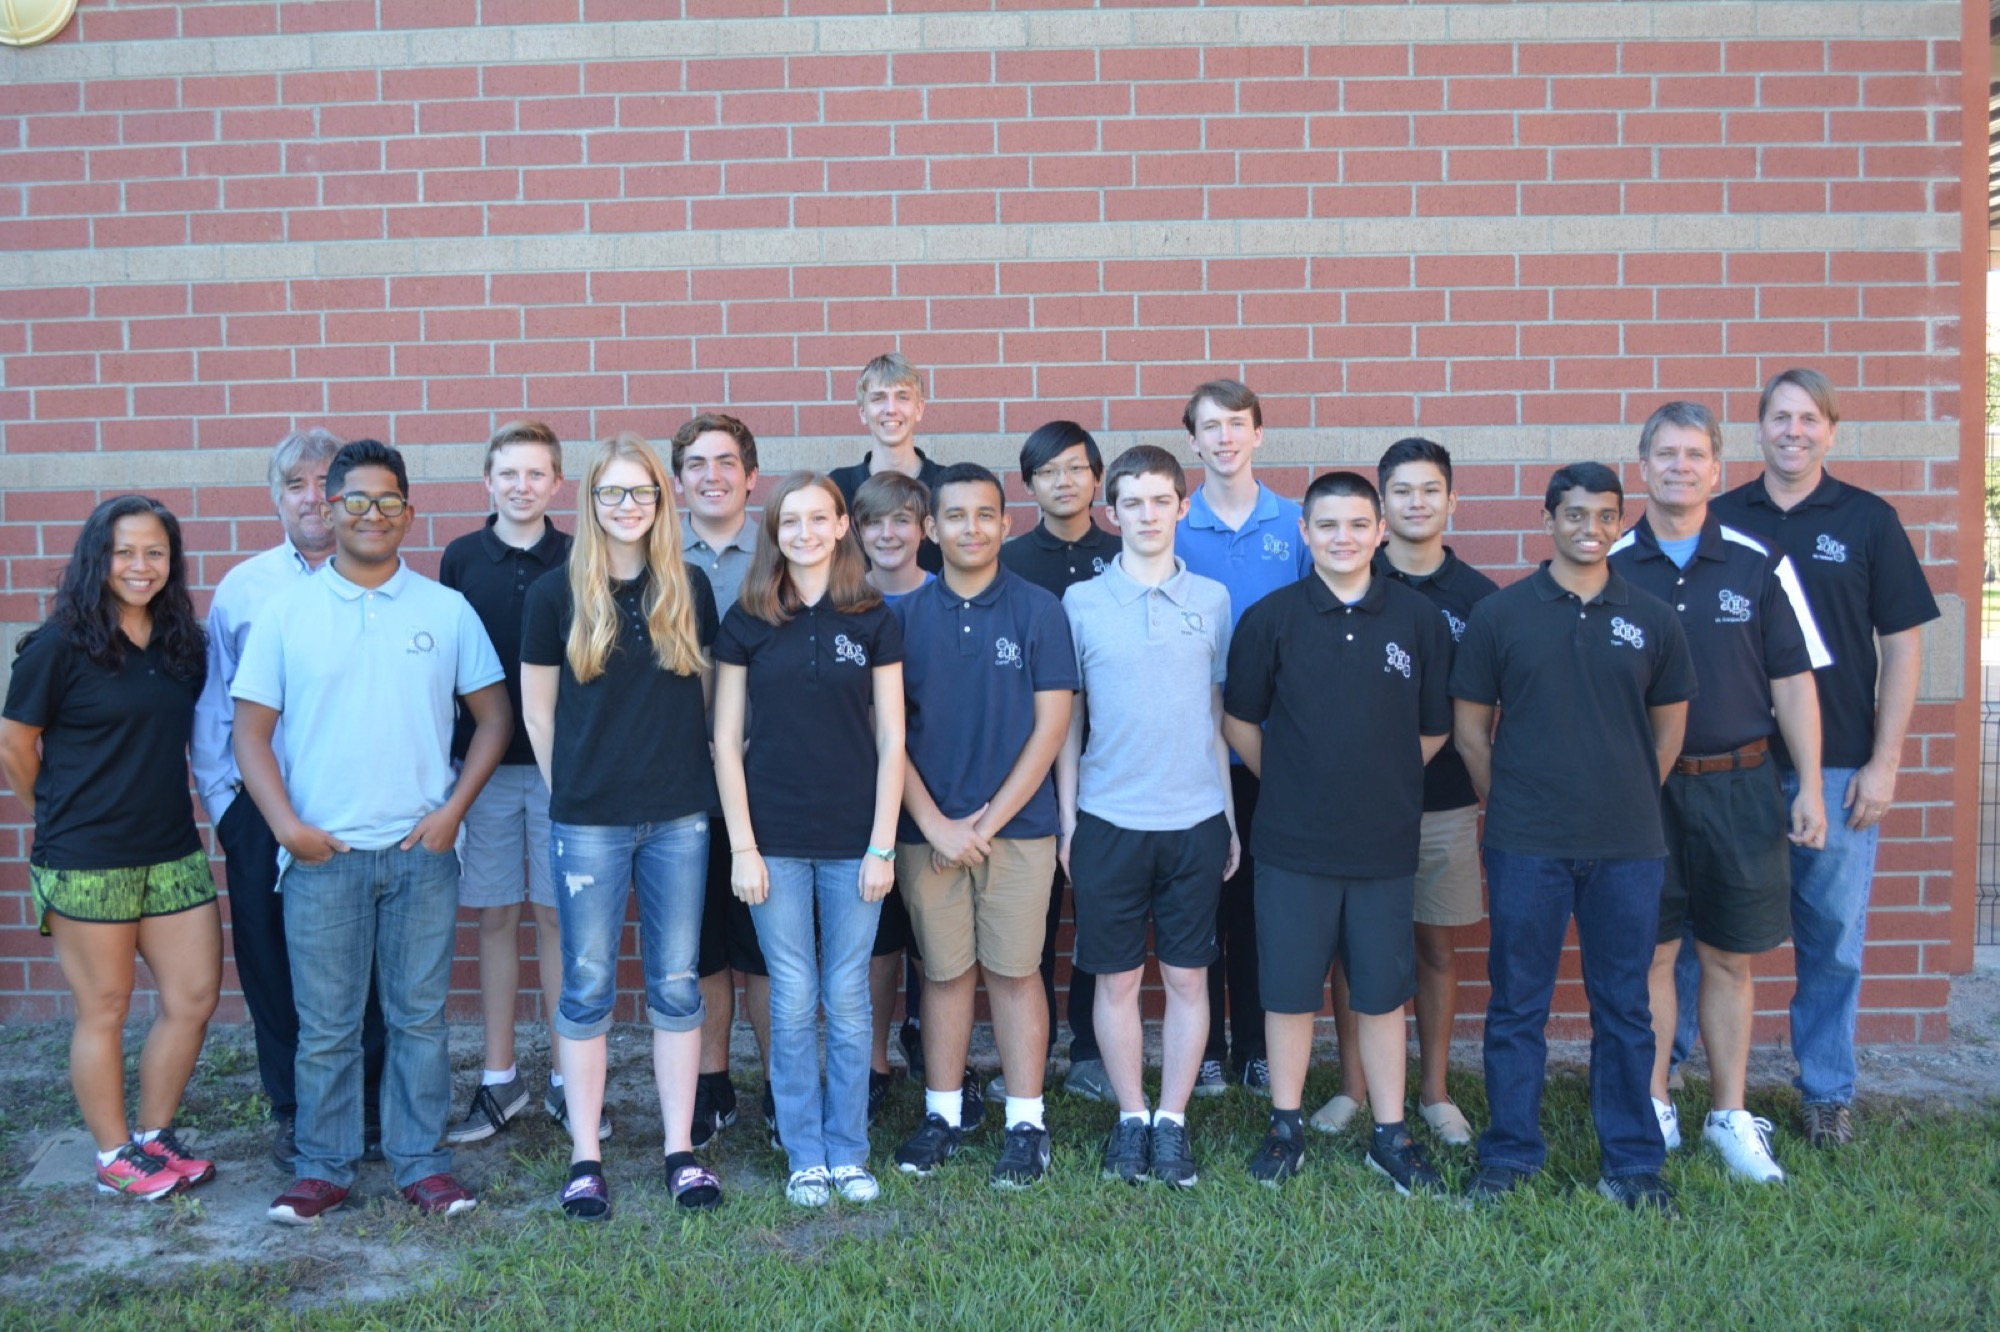
\includegraphics[width=0.8\textwidth]{Team4717.JPG}
% %\end{figure}

% \indent
% Within Hagerty High School, there lurks an atmosphere of surreptitious energy; the sounds of tinkering and hushed sibilation erupt in the dead of night, and shadowy hooded effigies loom around every corner. Who are these mysterious figures? These are the Mechromancers; they bring robots to life. Their codename: Team 4717. This team is undoubtedly a team full of effort, passion, and drive exemplified through their every action in the engineering process, outreach efforts, and competitive edge. The Mechromancers' main objective this year was to build a robot that was able to \hl{scale the crater, recover minerals, and shoot into the lander both quickly and accurately. Our robot's name this year is Bullseye, the second generation from the legendary Woody from 2016-17's Velocity Vortex.} We thought of keeping the Toy Story theme alive this year with having name of Bullseye be Woody's trusted steed, as well as being able to shoot with pin point accuracy.  

% \noindent
% \newline\textbf{\large Team Features:}
% \begin{itemize}
% 	\item \textbf{Extensive use of CAD} - Almost all parts of the robot were created in the Creo CAD software and built from raw materials. In Creo, movements are simulated using articulating joints, \textit{family tables} are used to create libraries of similar parts, \textit{skeletons} used for the top-down design, and all models are fully parameterized. \hl{Please view our design section, especially our page on the use of body and motion skeletons for the stabilization arms on page {\pageref{Stabilize:1}} to see an in-depth analysis on each mechanism in PTC Creo.}
%     \item \textbf{Outreach} - This year, our outreach team wanted to focus on promoting FIRST's values and the love for STEM and engineering in the community by making connections to other teams and our community in order to spread the values of FIRST and STEM. \hl{Refer to our Outreach Section to see our previous outreach events of this season, and learn about how we strive to build connections with businesses and organizations in our efforts to diffuse STEM across the world. For example, see how we founded and mentored an FLL Jr. Team on page {\pageref{FLLJR:1}}.}
%     \item \textbf{Organization} - We decided to keep our team organized through job specialization, breaking up into committees and subcommittees for each aspect of our team. This allows us to work in parallel while still working together. \hl{Check out our Committee Breakdown on page {\pageref{committees:1}} to learn about how the team is organized into these smaller committees, the role that each committee plays, and the members they consist of.}
%     \item \textbf{Custom Parts} - We used 3D printing as well as the laser cutter and machine shop at the University of Central Florida's Innovation Lab to create custom parts for the robot. \hl{Check out our Custom Parts Reference on page {\pageref{CustomPartsReference:1}} for the Creo sketch and CAD model of each part on our robot.} 
%     \item \textbf{Unique Notebook Format} - We use the \LaTeX typesetting language to create an engineering notebook that can be easily edited and formatted. We use Github to easily edit and share code.
%     \item \textbf{Always Evolving} - The Mechromancers are always yearning for innovative solutions to whatever issues we may face in competition, and therefore are always evolving. \hl{Refer to our Competition Section and our timeline on {\pageref{timeline:1}} to see how we evolved throughout the season.}
% \end{itemize} 

% \noindent \hl{Judges! Please be sure to check out the tabbed pages! We have included a description of the tabs in a table on the reverse side of this summary.} 

% Check out our robot \textit{Bullseye's} evolution through our design and build process in the upper right hand corner of each new meeting in the engineering section!
 
% \interestingpagetable 


%        ____  _           
%       |  _ \(_)          
%       | |_) |_  ___  ___ 
%       |  _ <| |/ _ \/ __|
%       | |_) | | (_) \__ \
%       |____/|_|\___/|___/
                    
\cleardoublepage
\section{Bios}
\vspace{3em}
\begin{minipage}[c]{\linewidth}
\centering
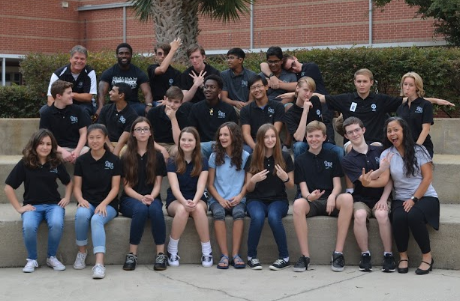
\includegraphics[width=\linewidth]{Images/Team/Team_Bios.PNG}
\end{minipage}
%\cleardoublepage
% Team Bios 3 girls 11 boys 

% #1 - name
% #2 - HeadShot image
% #3 - Interests
% #4 - Sub-Team
% #5 - Year
% #6 - Biography
% #7 - Picture #1
% #8 - Picture #2
\insertbio
{Ratam Rana}
{Dummy.png}
{Tennis}
{Software}
{Junior}
{
Ritam is a Junior at Hagerty High School, and this is his 3rd year involved with FTC Team 4717. He joined the robotics team because he loves to learn and discover new things about STEM. He has lots of interests in programming and design. He wants to pursue Computer Science and business in the future.
}
{Dummy.png}
{Dummy.png}


% % Coaches

% \insertbiomentor{Po Dickison}
{Po.JPG}
{Media Specialist}
{Team Sponsor}
{Robotics}
{
Po Dickison is a wonderful mentor. Mrs. Dickison works as the Media Specialist for Hagerty High School. She has over 18 years of experience in education and is passionate about STEM technology and learning. In addition to her Media position, Mrs. Dickison sponsors the Hagerty Robotics Program and the Future Educators of America Honor Society. She has presented at State and National level Technology conferences. In her spare time, she likes to read, shop, spend time with her family, and travel; however, due to her dedication to robotics, we make sure she has little spare time. We really love her, and she rakes in the cash for Hagerty Robotics. Without her, the teams’ robots would be made of duct tape and zip-ties. “I’m coaching Hagerty Robotics because I really want kids to go into the STEM field, it’s something that’s becoming the future.”  \\
}

% \insertbiomentor{Stefan Ibarguen}
{Stephen.JPG} 
{Computer Science and \newline Robotics Teacher} 
{Team Sponsor} 
{Robotics, Programming}
{
Stefan Ibarguen is a mentor for the Hagerty Robotics Program.  He started as a mentor with Hagerty Robotics in 2013 when teaching AP Computer Science and Robotics classes at our school.  He is no longer teaching classes, but continues as a mentor for the program because it is the most rewarding part of working at Hagerty High School.  The challenge of trying to bring order to the natural chaos of a group of highly talented high school teenagers is one that he relishes.  Before coming to Hagerty, Mr. Ibarguen spent many years at the Veritas corporation working in software development.  \\
}

% %  Mentors

 \insertbiomentor{Don Harper}
{Don.PNG}
{Director of UCF's TI \newline Innovation Lab}
{Mentor} 
{Sailing, Robotics}
{
Pursuing robotics and engineering as a personal passion and as his profession, Mr. Don Harper is our technical mentor, providing guidance and leadership to the team in software and hardware design. With Mr. Harper around, you will NEVER be bored. He won't let you! Mr. Harper loves challenges, and finding innovative solutions to problems. He is no stranger to robotics competitions. He remodeled his wife's car into an autonomous car, which earned him a spot in the finals of the DARPA Urban Challenge with the lowest budget of the whole competition. He's also been on the BattleBots TV show with his robot, and has been mentoring our team for over 5 years! Besides robotics, one of his favorite hobbies is sailing. As a 16 year old, he sailed a 16-foot catamaran all the way to the Bahamas!
}

% \include{Bios/M_EdgarMadruga}
% \insertbiomentor{Jaynelle Miller} 
{Jaynelle.JPG} 
{ASF Executive Assistant} 
{Notebook Mentor} 
{Robotics}
{
Ms. Miller is our Communications/Engineering Notebook Mentor. This is her ninth year mentoring an FTC team, her second mentoring Hagerty Robotics. Ms. Miller works for the Astronaut Scholarship Foundation. With STEM playing an ever increasing role in our everyday lives, Ms. Miller felt it was important to encourage her kids and other youth to participate in FIRST programs. She loves mentoring and learning right alongside the youth. In her free time, Ms. Miller enjoys running, gardening, sewing, and spending time outdoors with her family.
}

% \include{Bios/M_JakeMiller}




%         _____                          _ _   _            
%        / ____|                        (_) | | |           
%       | |     ___  _ __ ___  _ __ ___  _| |_| |_ ___  ___ 
%       | |    / _ \| '_ ` _ \| '_ ` _ \| | __| __/ _ \/ _ \
%       | |___| (_) | | | | | | | | | | | | |_| ||  __/  __/
%        \_____\___/|_| |_| |_|_| |_| |_|_|\__|\__\___|\___|
                                                     
                                                    
\clearpage 
\pagestyle{plain}
\noindent\textbf{\Huge Committees}
\addcontentsline{toc}{section}{\numberline{}Committees}
\newline

\interesting{}{committees:1}
\noindent\textbf{\Large Design Committee -} Jonathan Valentin, Shey Naik, Clayton Workman, Mason Dettman \\ Responsible for designing parts and assemblies within PTC Creo, and simulating robot movement. \\
\newline\noindent\textbf{\Large Hardware Committees -}
\\ Responsible for building the external and physical components. Lead by team leader Sam Jones and Chief Engineer Shey Naik, mentored by Mr. Harper and Mr. Ibarguen.\\

\begin{itemize}

\item \textbf{Drivetrain Committee-} Shey Naik, Austin English, Mason Dettman, Haven Carter. \\ Responsible for designing and creating the base drivetrain.

\item \textbf{Intake Committee -} Benjamin Steinebronn, Jonathan Valentin, Clayton Workman, Sam Jones.  \\ Responsible for designing and creating the intake mechanism. 

\item \textbf{Shooter Committee -} Shey Naik, Jolie Miller, Mason Dettman, Haven Carter. \\Responsible for the design and assembly of the shooter. 

\item \textbf{Hang Committee -} Benjamin Steinebronn, Mason Dettman, Shey Naik, Jonathan Valentin, Alex Eum. \\  Responsible for designing and creating a hang mechanism to latch and delatch from the lander. 

\end{itemize} 

\noindent\textbf{\Large Control Committees -} \\ Responsible for the programming, wiring and the sensors involved within the robot that provide and enhance control. 

\begin{itemize}

\item \textbf{Wiring Committee -} Ben Steinebronn, Lillian Sullivan, Drew Demaggio. \\ 
Responsible for the connection and management of the wires on the robot. 

\item \textbf{Sensors Committee -} Shey Naik, Ryan Nelson, Alex Eum, Jolie Miller, Haven Carter. \\
Responsible for configuring and attaching servos and sensors onto the robot for teleop and autonomous functions. 

\item \textbf{Programming Committee -} Ryan Nelson, Alex Eum, Jolie Miller. \\ Responsible for coding the autonomous and teleop functions. 

\end{itemize} 

\noindent\textbf{\Large Scouting Committee -} Drew DiMaggio, Lillian Sullivan, Gabby Herrera, Falon Jones \\
Responsible for assessing other teams' robot performance and gathering data essential for alliance selection. \\
\newline\noindent\textbf{\Large Notebook Committee -} Haven Carter, Shey Naik, Mason Dettman, Ben Steinebronn, Jolie Miller.  \\
Responsible for creating the framework of the engineering notebook, fixing syntax errors within \LaTeX, and editing the daily entries. Lead by Notebook Lead Haven Carter and mentorship provided by Mrs. Miller. \\
\newline\noindent\textbf{\Large Outreach Committee -} Jolie Miller, Gabby Herrera, Falon Jones.  \\
Responsible for coordinating outreach events, responding to emails received at hagertyrobotics@gmail.com, and demonstrating the robot at events. Mentorship provided by Mrs. Dickison. \\
\newline\noindent\textbf{\Large Communications Committee -} Jolie Miller, Haven Carter, Austin English.  \\
Responsible for running the Hagerty Robotics Twitter, Instagram, and website. Lead by Head of Communications Jolie Miller and mentorship provided by Mrs. Miller. \\

%         _____                                    
%        / ____|                                  
%       | |     ___  _ __  ___ 
%       | |    / _ \| '_ |/ _ \
%       | |___| (_) | |   | __/ 
%        \_____\___/|_|   \___|

\cleardoublepage
%\chapterstyle{hhs_blank_chapter}
\section{4717's Core Values}
\vspace{3em}
\begin{minipage}[c]{\linewidth}
\centering

\includegraphics[width=\linewidth]{Core_Values/CV_Title.PNG}
\end{minipage}
%\insertCV{Discovery}
{Every day I walk into the robotics room, I get to learn new concepts and apply old ones I'd only ever been lectured about.}{Mason Dettman, 11}
{Us Mechromancers love to learn new things, and each of our members comes in everyday with a ready mind set. Our team shows discovery through our pursuit of knowledge. For example, at one meeting we asked an engineer to come in and teach our team how to solder. We also discovered a lot through our unique drivetrain design. By having an unusual design, our team gained insightful knowledge of physics and gyros. }
{
\item[$\blacksquare$] Page \pageref{Discovery:1}
 \item[$\blacksquare$] Page \pageref{Discovery:2}
 }
{Discovery/discovery1.jpg}{Discovery/IITSEC_1.jpg}
\insertCV{Impact}
{Outreach is a fundamental part of our team, and it's honestly crazy to see the ripples we create within the community.}{Ben Steinebronn, 10}
{Though we may seem dark and sinister, Mechromancers pride ourselves in making our community a lighter place with our Outreach program. Within our small Oviedo community, our impact has not gone unnoticed. We’ve had over seven hundred hours of service to our community, and through it we’re touched hundreds of lives. At the core of our Outreach program is inspiring possible future Mechromancers with robotics and all they can accomplish in it. By introducing younger students to FIRST through our mentorship programs, we get to see a love for learning come to life inside each of these students. }
{
\item[$\blacksquare$] Page \pageref{Impact:1}
\item[$\blacksquare$] Page \pageref{Impact:2}
}
{Impact/impact1.jpeg}{Impact/impact2.JPG}
\insertCV{Fun}
{The Mechromancers are like my second family. Sure, we work together, but we also have fun together.}{Jolie Miller, 10}
{While some may assume Mechromancers are all work and no play, they will soon find a much more lighthearted side to this sinister squad. We find delight in the innovation and discovery opportunities we gain everyday through our program. It might be a little cliche, but we couldn’t love our team more. As they say, FIRST is the hardest fun we’ll ever have.}
{\item[$\blacksquare$] Page \pageref{fun:1}
 \item[$\blacksquare$] Page \pageref{competition:3}
 \item[$\blacksquare$] ANY of them! We have fun on the daily :)}
{Fun/fun1.JPG}{Fun/fun2.jpg}


\insertCV{Innovation}
{The Mechromancers always shake things up and find a crazy new approach to a challenge. That's what excites me the most as a member.}{Jonathan Valentin, 12}
{Due to its intriguing design, our robot, Bullseye, tends to turn a few heads. The first thing an individual notices when they see Bullseye is it’s big wheels. The reason behind this unusual choice is the innovative opportunities it provided, as well as its potential efficiency. Our drivetrain is like no other team we’ve ever encountered, and our free floating chassis are just some of the ways we innovate as we design.}
{\item[$\blacksquare$] Page \pageref{innovate:1}
 \item[$\blacksquare$] Page \pageref{innovate:2}
 \item[$\blacksquare$] Page \pageref{innovate:3}
 }
{Innovation/inno1.PNG}{Innovation/inno2.JPG}
\insertCV{Inclusivity}
{Everyone has a duty and responsibility on the team, and I think that's what makes us special}{Haven Carter, 12}
{As a practically ancient team, Mechromancers have grown over the years to include people from different walks of life. We began as an all girls team called Estrogenius, and over the years, we’ve risen anew to include a variety of genders, ethnicities, countries of origin, and skills on our team. It’s incredibly important to us that we maintain diversity and positivity in everything we do. We also strive to include every team member in all parts of robotics especially the freshman students. By the end of the build season, us members are practically family.}
{
\item[$\blacksquare$] \pageref{Inclusivity:1}
\item[$\blacksquare$] \pageref{FLLJR:1}
\item[$\blacksquare$] \pageref{Inclusivity:3}
}
{Inclusivity/FLL_Jr_Mentoring_1.jpg}{Inclusivity/inclusive_lesson.jpg}

\insertCV{Teamwork}
{When the whole team comes together, anything is possible. I love that.}{Lillian Sullivan, 9}
{Teamwork lies at the heart of every loyal Mechromancer. Team unity is something we struggle with at times, due to members being so different, but it is a challenge we have actively worked to overcome. Using a communication app called Band, as well as a business management app called Trello, we work to remain united and merged in team spirit. Mechromancers Rise! }
{\item[$\blacksquare$] Page \pageref{teamwork:1}
 \item[$\blacksquare$] Page \pageref{committees:1}
 \item[$\blacksquare$] Page \pageref{connect:1}
 }
{Teamwork/Teamwork1.jpg}{Teamwork/Teamwork2.JPG}

\cleardoublepage

%Workspaces
%Showcases the three primary workspaces utilized by the team 
%\clearpage
\addcontentsline{toc}{section}{\numberline{}Our Workspaces}
\subsection*{\textbf{\Huge Our Workspaces:}}
\vspace{.2cm}
%\begin{flushleft}
\setlength{\parindent}{.25in} 
% guidelines http://www.firstinspires.org/sites/default/files/uploads/resource_library/ftc/2016-2017-season/engineering-notebook-guidelines.pdf
% starts at bottom of page 12

\textbf {\Large Our Workspaces:}
\newline
The Mechromancers primarily utilize three workspaces to meet, design and build throughout the competition season.  Two of these workspaces, the UCF Innovation Lab and Machine Shop in Engineering Building II, are courtesy of our mentor Mr. Harper, who is the director of the Innovation Lab and a licensed machinist who helps our team greatly. Our main workspace, used for official team and club meetings, is in the Industrial Arts Lab at Hagerty High School. This is where the team designs, builds, innovates and grows throughout the year. This is also where we have a full field setup, allowing us to practice and test freely. The Mechromancers are thankful for having access to these resources, as they contribute greatly to our success. Below, you can learn about each of these workspaces in detail.

\textbf {\large Media}
%  \begin{figure}[h!]
%  \centering
%    \includegraphics[width=0.4\textwidth, angle=0]{Meeting/January/01-10-17/Cap_Ball_Lifter_Drawing.png}
%   \caption{Hand drawing of claw grabber and cap ball mechanisms}
%   \label{fig:Cap_Ball_Lifter_Drawing}
%  \end{figure}

\subsection*{Description}
The Industrial Arts Room in Hagerty High School, room 123 in Building 6, is our main meeting room and workspace. This is where the team constantly congregates througout the year for our official biweekly meetings on Tuesdays and Thursdays, discussing team and club updates before breaking off into our teams and committees to work, create, and build. We keep toolboxes and equipment in the closet as well as wood spares for quick replacements. We also have computers installed with PTC Creo for CAD, and have online access to our notebook through Overleaf. Since we mainly use this room for design, we also have plenty of drawing boards and laptops for the team discuss, collaborate, and hash out ideas with the team. 

\textbf {\large Hagerty's Industrial Arts Room}
%  \begin{figure}[h!]
%  \centering
%    \includegraphics[width=0.4\textwidth, angle=0]{Meeting/January/01-10-17/Cap_Ball_Lifter_Drawing.png}
%   \caption{Hand drawing of claw grabber and cap ball mechanisms}
%   \label{fig:Cap_Ball_Lifter_Drawing}
%  \end{figure}

\subsection*{Description}
The Industrial Arts Room in Hagerty High School, room 123 in Building 6, is our main meeting room and workspace. This is where the team constantly congregates througout the year for our official biweekly meetings on Tuesdays and Thursdays, discussing team and club updates before breaking off into our teams and committees to work, create, and build. We keep toolboxes and equipment in the closet as well as wood spares for quick replacements. We also have computers installed with PTC Creo for CAD, and have online access to our notebook through Overleaf. Since we mainly use this room for design, we also have plenty of drawing boards and laptops for the team discuss, collaborate, and hash out ideas with the team. 

\textbf {\large UCF Texas Instruments Innovation Lab}
 \begin{figure}[h!]
 \centering
   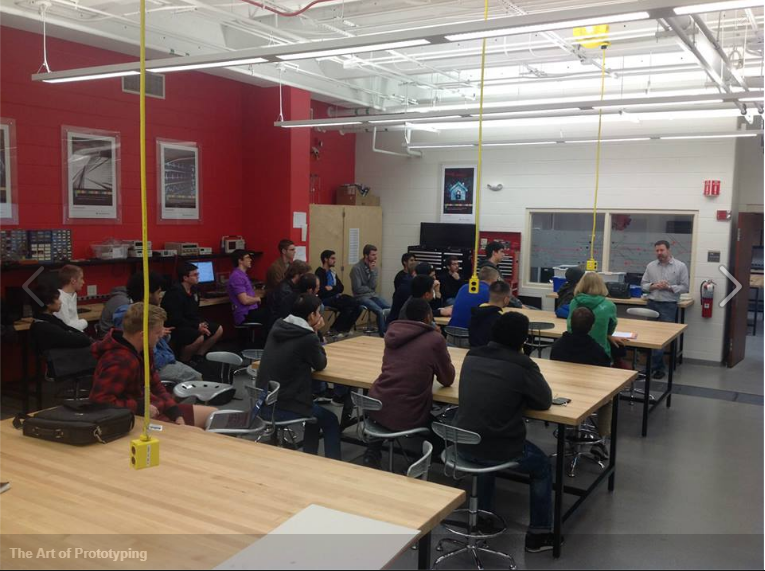
\includegraphics[width=0.7\textwidth, angle=0]{Workspaces/innovationlab.PNG}
  \caption{The UCF TI Innovation Lab, Courtesy of Mr. Harper}
 \end{figure}

\subsection*{Description}
The TI Innovation Lab, found in Engineering Building II in the University of Central Florida, is a makerspace directed by one of our mentors, Mr. Harper. It provides us access to large workshop with a wide range of tools and equipment, along with a soldering station and wiring for electrical needs as well as our most utilized resource, a laser cutter. This is where the team can cut new parts, build and assemble under the guidance of our mentor. We can also prototype and test here, as it allows us to think and modify as we wish. The team often meets here for unofficial meetings occasionally on weekdays and weekends. 

\textbf {\large UCF Machine Shop}
 \begin{figure}[h!]
 \centering
   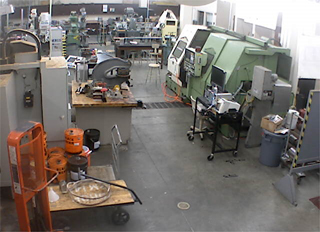
\includegraphics[width=0.7\textwidth, angle=0]{Workspaces/machine_shop.jpg}
  \caption{The UCF Machine Shop}
 \end{figure}

\subsection*{Description}
Right beside the TI Innovation Lab is the UCF Machine Shop, with heavy machinery like the lathe, the CNC Mill, drill press, and many more, all of which play a crucial role in making custom parts and pieces for our robot. With our mentor Mr. Harper also being a machinist, this is where the team learns from the best, using CAM tools to cut and create various pieces with ease. We use this machine shop throughout the season, whenever parts are required to be machined. This is a great workspace as it provides us with various resources that the team wouldn't even dream of having otherwise. It plays an essential role in our team's innovation and design. 



%         ____        _                       _     
%        / __ \      | |                     | |    
%       | |  | |_   _| |_ _ __ ___  __ _  ___| |__  
%       | |  | | | | | __| '__/ _ \/ _` |/ __| '_ \ 
%       | |__| | |_| | |_| | |  __/ (_| | (__| | | |
%        \____/ \__,_|\__|_|  \___|\__,_|\___|_| |_|
                                             
                                             
\cleardoublepage
%Outreach
%\chapterstyle{hhs_blank_chapter}
% \newcounter{outreach_hours}
\section{Outreach Section}
\vspace{3em}
\begin{minipage}[c]{\linewidth}
\centering
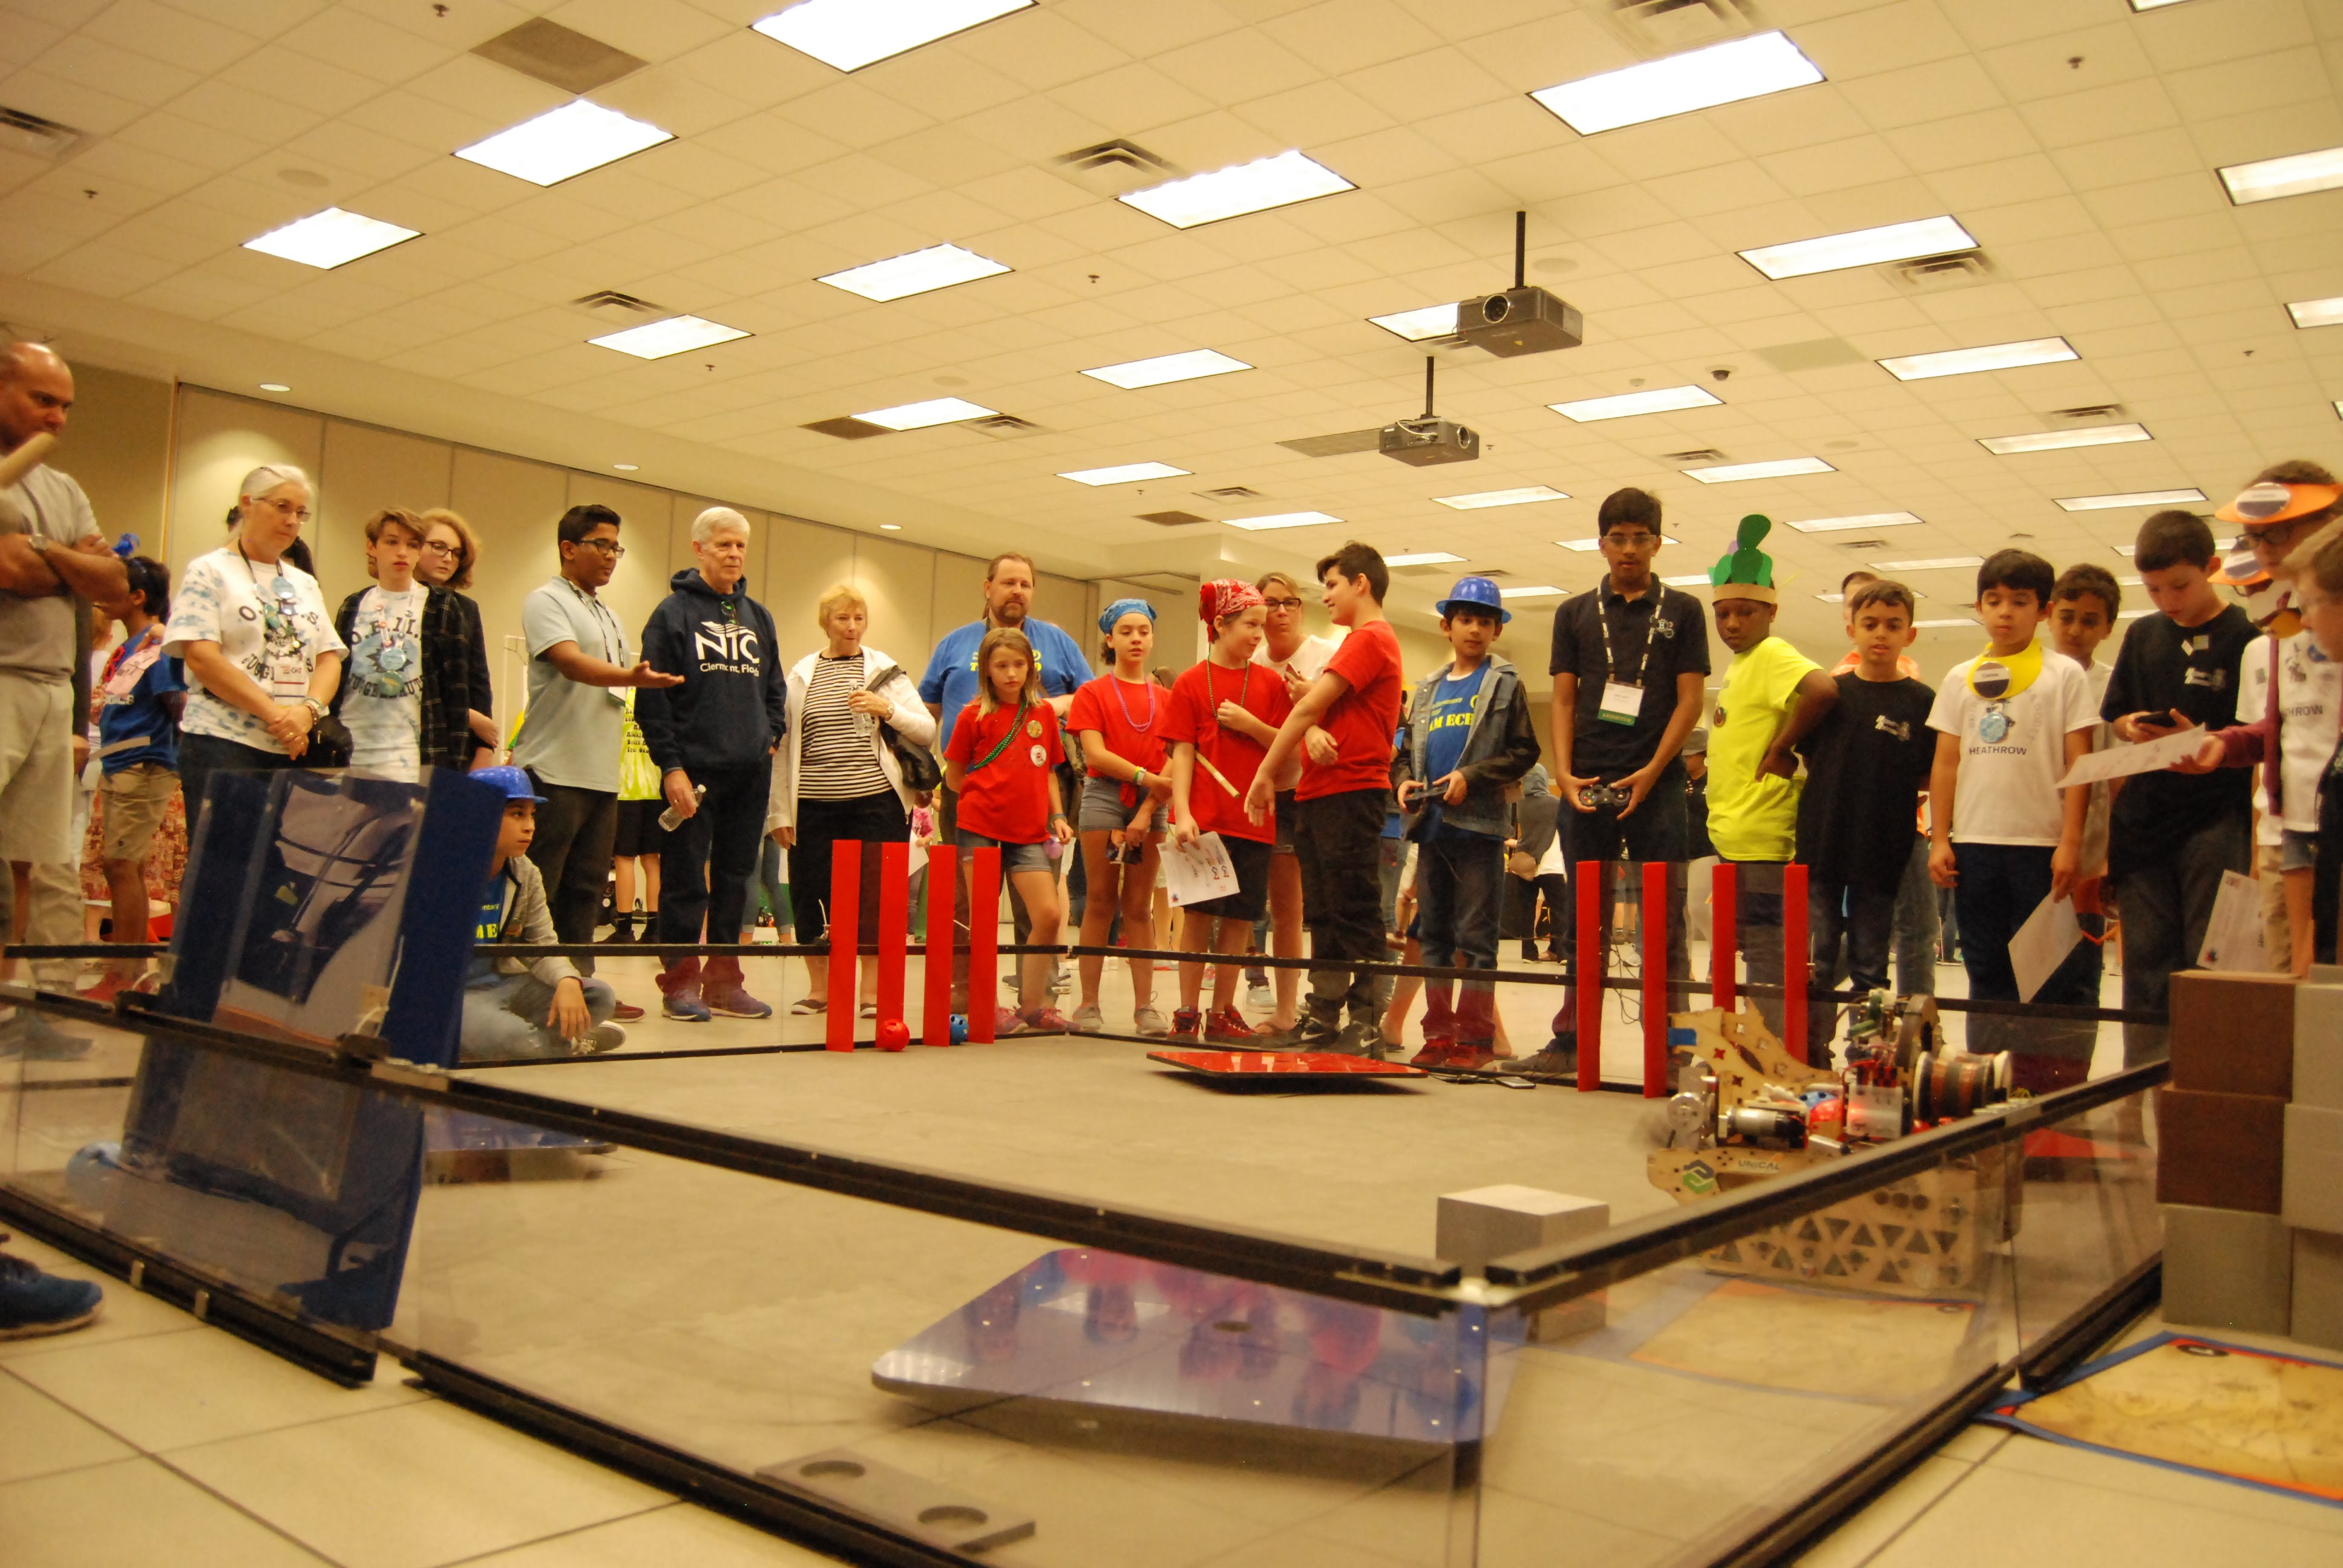
\includegraphics[width=\linewidth]{Images/Main/WoodyDemo.jpg}
\end{minipage}
%\include{Outreach/ASF_Apollo}
%\include{Outreach/}
%\cleardoublepage

%CURRENT OUTREACH
% \insertOutreachEvent{Lucerna Studios Stem Fair}
{04/29/18}
{6} 
{LC_STEM_Fair.PNG} 
{Make connections with entrepreneurs and business professionals in the STEM field, introduce attendeees to FIRST, interact with other presenters at the event} 
{
The Mechromancers had a spectacular opportunity to make connections at our first outreach event of the 2018-19 season at the Lucerna Studios STEM Fair, on April 29th, 2018. The team was invited to hold an exhibition at a STEM Fair for the launch of Lucerna Studios, an incredible new start-up with a library of academic VR/AR experiences and games that attempts to conquer kids' fear of learning and STEM through their passion for games. Held in downtown Orlando, we presented alongside our friends over on the FRC Team 1902 Exploding Bacon, demoing with partners in crime Woody and Buzz, our previous seasons robots, to children, parents and entrepreneurs at the event. The air buzzing with energy and conversation, the event was an amazing chance for our team to interact with business professionals in the STEM field as well as visitors, and introduce them to FIRST and the opportunities it provides to youth in terms of making STEM exciting, just as Lucerna Studios hopes to do. Overall, it was a fantastic experience that allowed us to meet our program's outreach goals for the year and develop local connections with those in our area. 
}
{LC_STEM_Fair_1.PNG}{LC_STEM_Fair_2.PNG}
% \include{Outreach/SCC_Tech_Night/Seminole_Tech}
% \insertoutreachHours{RoboBoat} 
{06/25/22}
{105}
{Roboboat/PXL_20220625_114745716.jpg}
{To continue growing our skills and spreading FIRST in the local community}
{Over the summer, our team participates in the weeklong, collegiate, international competition, RoboBoat. Through this competition, we grew our connections with the STEM community and increased our technical skills. Our programmers expanded to use Python instead of Java to work with the Robot Operating System (ROS) on Linux and implemented more electronics. Our hardware members elevated their CAD skills by designing a new and improved boat in the shape of a semicircle. This unique design really made us stand out. We placed 5th at RoboBoat. 
} 
{Roboboat/PXL_20220624_122113295.MP.jpg}
{Roboboat/PXL_20220623_174805269.jpg}

% \include{Outreach/ASF_Apollo_Prep/ASF_Apollo}
% \include{Outreach/Kids_Summer_Camp/Kids_Summer_Camp}
% \insertoutreachHours{Recruitment Camp} 
{08/01/22-08/05/22}
{37.5}
{Recruitment_Camp/PXL_20220802_141822442.MP.jpg}
{To connect with high schoolers and incoming high schoolers who are interested in joining the team}
{At our Recruitment Camp, we invite prospective team members to get a feel for our team and determine if joining would be a good fit for them. We teach high school students the basics of understanding hardware, 3D modeling, writing and running software, writing engineering notebook entries, designing multimedia projects, and creating successful outreach events. Students get a taste of the FIRST Tech Challenge experience and use the skills they develop from this camp to help our team, our sister team, or another community team they may join.
} 
{Recruitment_Camp/PXL_20220803_160342188.MP.jpg}
{Recruitment_Camp/PXL_20220803_172241401.MP.jpg}
% \include{Outreach/Rookie_Team_Crash_Course/Rookie_Team_CC}
% \include{Outreach/RMHC/RonaldMcDonald}
% \include{Outreach/RoboPegz_Mentoring/RoboPegz_Mentoring}
% \include{Outreach/Stenstrom_Elem_Demo/Stenstrom_Elem_Demo}
% \insertoutreachHours{UCF STEM Day} 
{10/21/22}
{6}
{UCF_STEM_Day/_d_351h61_d_j68Ud018svc1eixci9iss4f_3wd7c0.jpg}
{To spread STEM to the youth in our community}
{UCF Stem day is an event that the University of Central Florida hosts for kids in elementary and middle school. There are various stations where they can learn about science, technology, engineering and math. We reached out to the organizer of this event and we secured a place where we could hold a station about our robots. During the UCF STEM Day, we had two members from our team along with two from our sister team, team 4227 Metal Morphosis, went and presented to over 300 students across Central Florida. We had a place where kids could drive our robots, code EV3 robots and learn about other engineering techniques. 
} 
{UCF_STEM_Day/_d_351gfg_h_4j1Ud018svc90wkna1mux3_3wd7c0.jpg}
{UCF_STEM_Day/_d_351h30_d_868Ud018svcd06s3v3ylhr6_3wd7c0.jpg}
% \insertoutreachHours{FLL JR. Mentoring} 
{Every Friday Starting 08/10/21}
{44}
{FLL_JR_Mentoring/IMG_8857.JPG}
{Create and develop local connections by volunteering for a greater cause; exemplify FIRST's Core Values within the community} 
{Our youngest team is our four-member FLL Discover team. These students are new to the world of STEM, and it is our job as mentors to provide them with the guidance necessary for their success in the future. Through the use of Lego bricks and fun activities, they have developed a foundation for understanding the Core Values of FIRST, the Engineering Design Process, and Gracious Professionalism. Although these may be big words for our young students, we ensure that our lesson plans allow the students to have fun while learning many new concepts. Most memorably, we spend the first few minutes of each meeting providing the students with a set of 12 colorful Lego bricks. This activity allows the students to express themselves, but in a way that requires them to think in out-of-the-box ways. They learn to discover new ways to build items like chairs, birds, and bridges under the restriction of just 12 bricks. Another session project that helps the students develop innovation skills is the Explore Building Session conducted after each lesson focusing on a transportation concept. Students are tasked with projects from their notebooks and are encouraged to build the vehicles and buildings they design. Then, following their building period, the students share their creations, often working together to simulate the transportation of cargo and vehicles across the Cargo Connect mat. This activity allows them to experience cooperation in an inclusive team environment, which is a skill that will support them now and in the future.

} 
{FLL_JR_Mentoring/IMG_8865.JPG}
{FLL_JR_Mentoring/IMG_8866.JPG}
\interesting{}{FLLJR:1}
% \include{Outreach/Maker_Faire/Maker_Faire}
% \include{Outreach/B&N_Expo/B&N_Expo}
% \include{Outreach/IITSEC/IITSEC}
% \include{Outreach/JHMS_STEAM_Night/JHMS_STEAM_Night}
% \insertoutreachHours{FLL Challenge Teams} 
{Tuesdays and Fridays Since 08/10/21}
{66}
{FLL_Team_Mentoring/FLL.JPG}
{We have three student-led FLL Challenge teams in our Junior Robotics program here at Hagerty High School. During this robotics season, we have witnessed each member thrive and grow in their knowledge of STEM.}
{We have three student-led FLL Challenge teams in our Junior Robotics program here at Hagerty High School. During this robotics season, we have witnessed each member thrive and grow in their knowledge of STEM. The most important lessons we teach them come from our collective knowledge of FIRST and STEM. A lot of us mentors started our journey in FIRST LEGO League as elementary and middle school students. Watching them start their journey is a reminder to us of the impact we can make on our members. We teach the FIRST essentials, such as core values, gracious professionalism, the design process, and team building. We teach core values and gracious professionalism throughout the year but we like to do so in a way that the kids will really learn what it all means. For example, we play telephone to show them how words can change without the crucial element of communication. In addition, we go through a thorough lesson about different robot parts and how they interact. For example, we taught about how gears mesh and can change direction. We teach about the design process and where they collaboratively design a robot, and teach them about specific lessons such as the importance of failure and using it as an advantage.  

} 
{FLL_Team_Mentoring/FLL_1.JPG}
{FLL_Team_Mentoring/FLL_2.JPG}
% \include{Outreach/Plaid_Mentoring/Plaid_Mentoring}
% \insertoutreachHours{FLL Tournament} 
{12/10/22}
{7}
{FLL_Tournament/PXL_20221210_182016903.MP.jpg}
{To volunteer at different FIRST events in our community.} 
{One thing we pride ourselves on is our mentoring of FLL teams. We have one FLL Discover team, four FLL Explore teams and three FLL Challenge teams. With FLL Challenge, we have been able to teach these young students how to build and program Lego Mindstorms EV3’s to complete missions on the board. We have three different Challenge teams but unfortunately they were not able to all go to the same FLL qualifier. We had two of our newer Challenge teams, the “WARNELB Bros” and Dino Nuggies go to a qualifier on the same day as an FTC Meet. Because of this we were unable to send team members to their qualifier. Though we did not have members go with them we were able to send one of our mentors, Ms. Po, to go with them to make sure they knew what they had to do and were able to get to the judging room on time. Unfortunately neither of these two Challenge teams were able to move past their qualifying tournament which made us put a lot of hope into our third Challenge team, the Minimancers. Two weeks later we had our second Challenge Qualifier, the Exploding Bacon Qualifier. This qualifier was a very intense tournament because it had a lot of the heavy hitting Challenge Teams like the teams from Jackson Heights Middle School, Teams 920 and 10240. At the end of the tournament it turned out that the Minimancers did not move on either which was quite unfortunate. Though none of our FLL Challenge teams moved on, we have decided to continue having meetings until April. Our reasoning for this was to give the newer Challenge members the ability to learn more about coding and building a sturdy robot in the hopes that next year they will be able to move on and qualify for their Regional Tournament.
} 
{FLL_Tournament/PXL_20221210_141230250.MP.jpg}
{FLL_Tournament/PXL_20221210_172656038.MP.jpg}

% \include{Outreach/Girls_in_Engineering/GirlsinEngineering}


 %           ____            _                       _____           _            
 %          |  _ \          (_)                     |  __ \         | |           
 %  ______  | |_) |_   _ ___ _ _ __   ___  ___ ___  | |__) |_ _ _ __| |_   ______ 
 % |______| |  _ <| | | / __| | '_ \ / _ \/ __/ __| |  ___/ _` | '__| __| |______|
 %          | |_) | |_| \__ \ | | | |  __/\__ \__ \ | |  | (_| | |  | |_          
 %          |____/ \__,_|___/_|_| |_|\___||___/___/ |_|   \__,_|_|   \__|         
                                                                                                                                                           
\cleardoublepage
\part{Business Section}
\vspace{3em}
\begin{minipage}[c]{\linewidth}
\centering
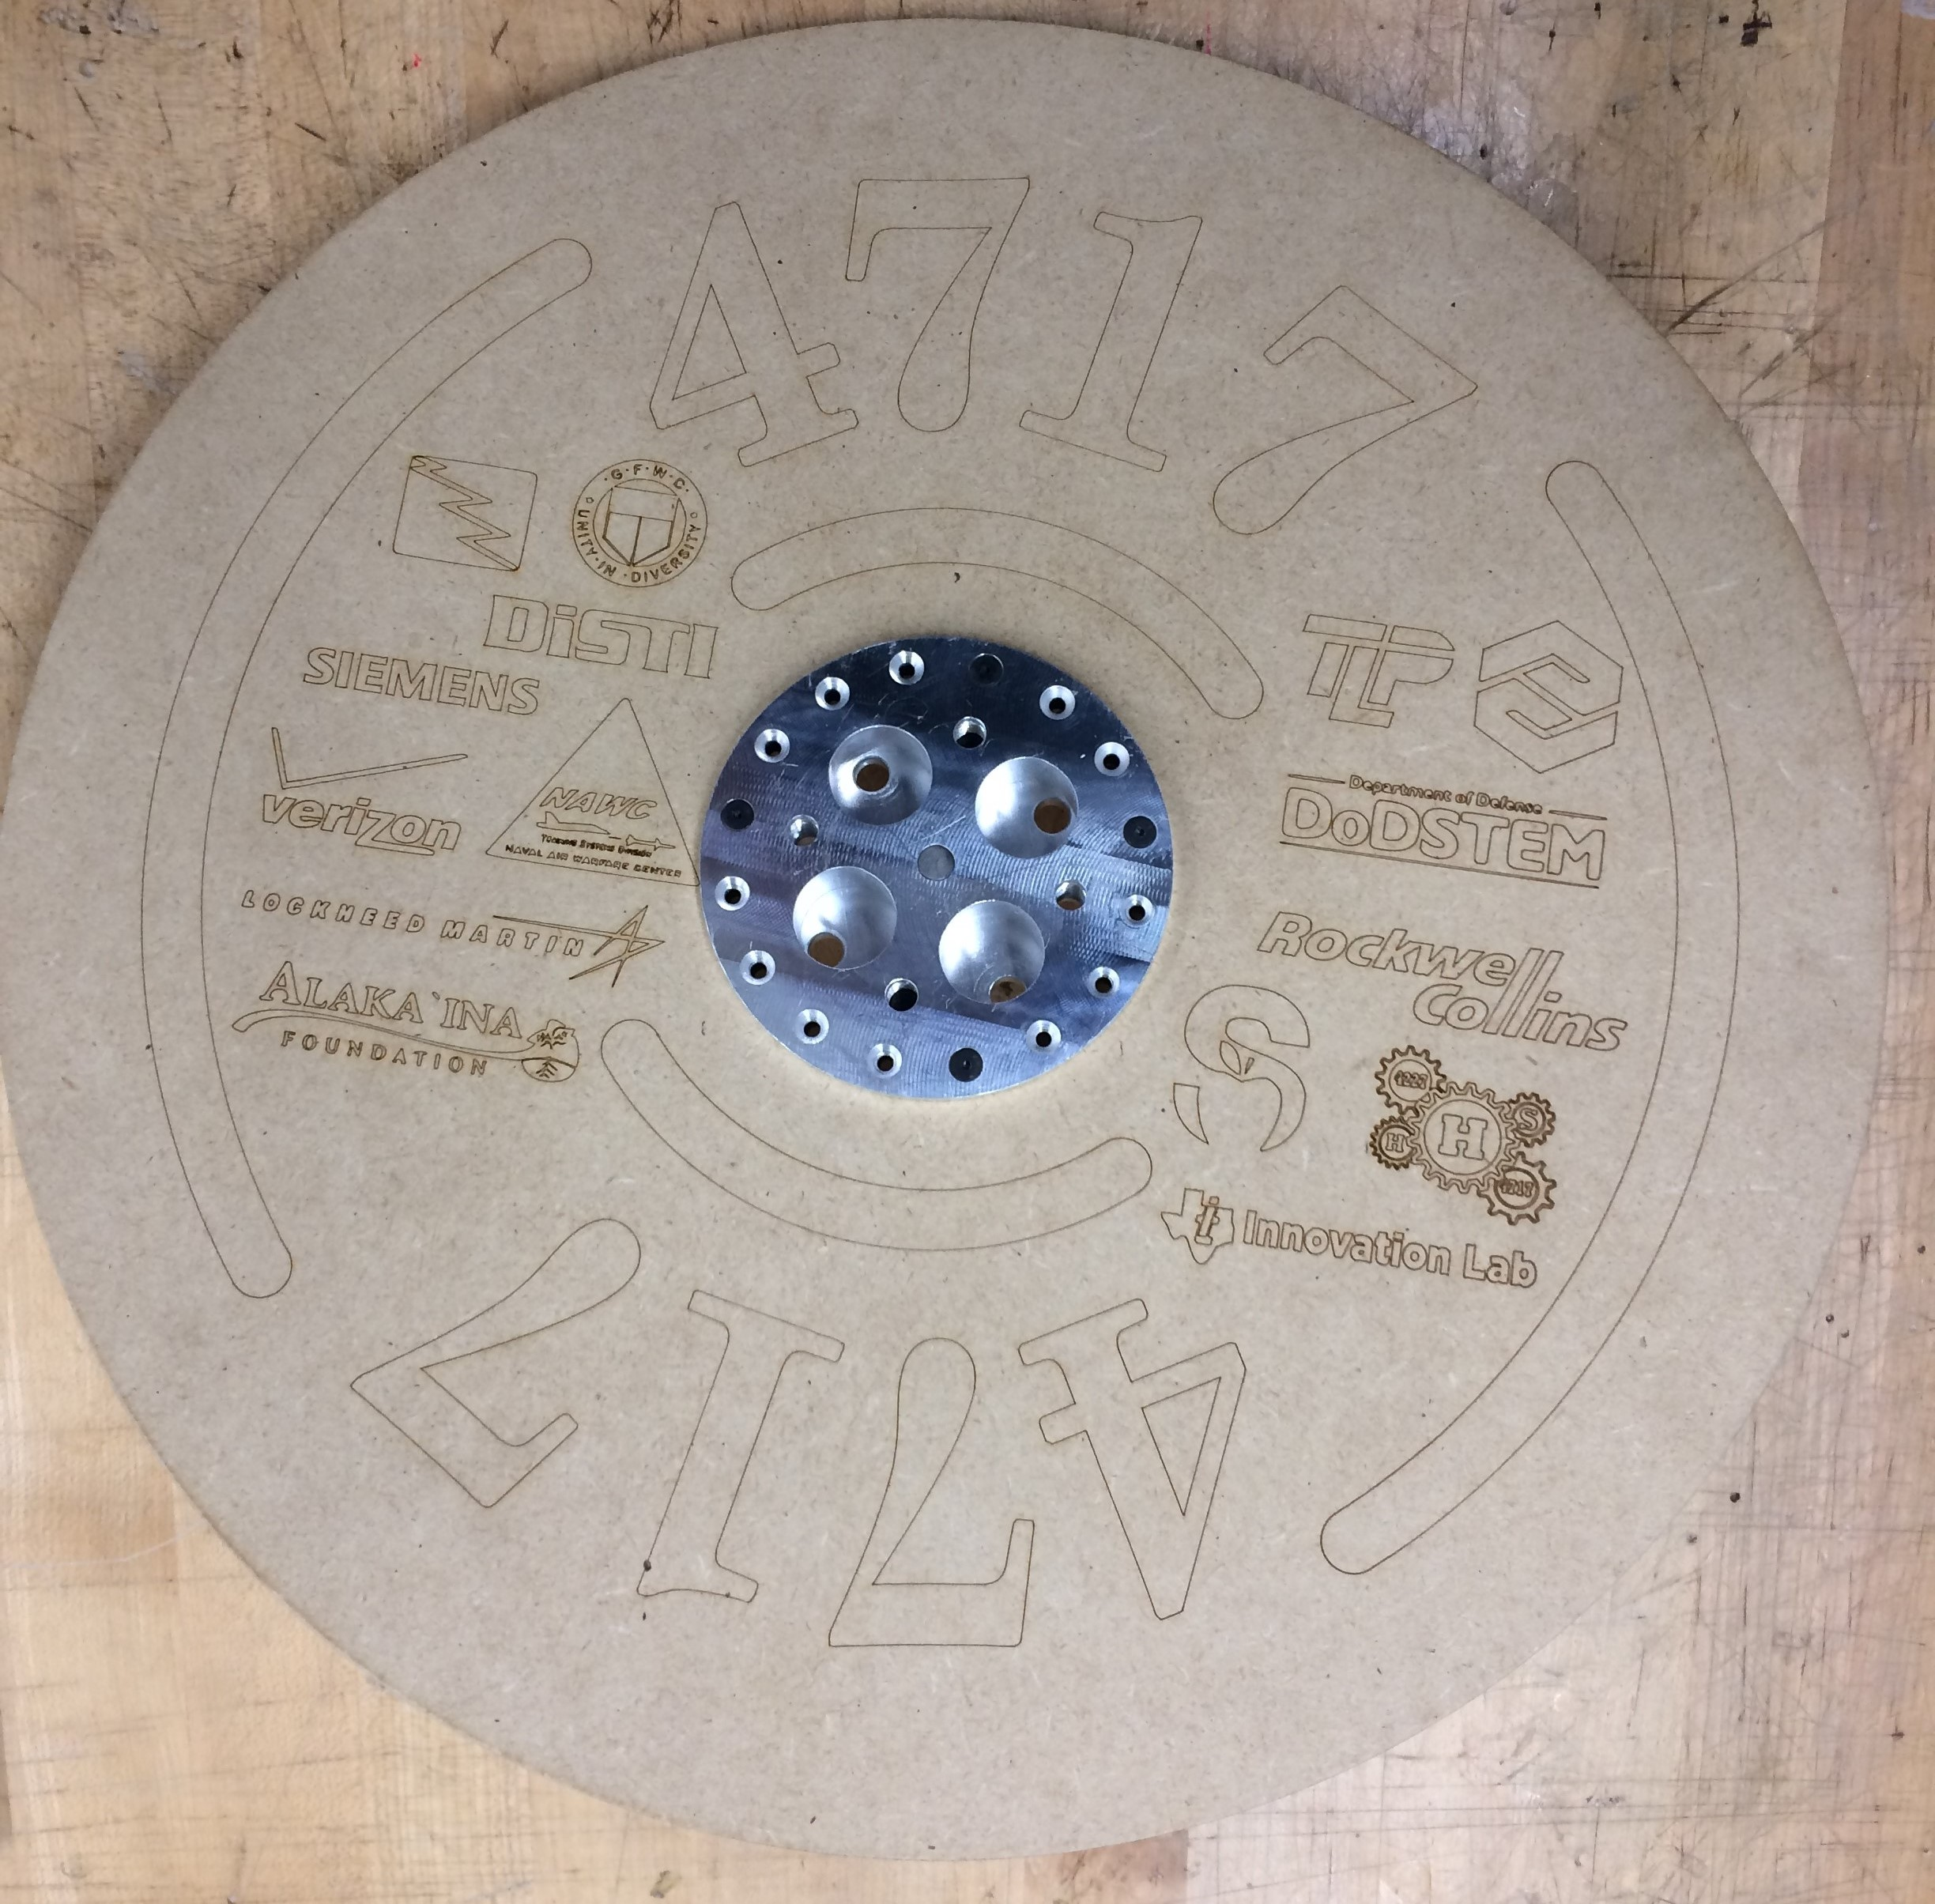
\includegraphics[width=\linewidth]{Images/Main/Big_wheel.JPG}
\end{minipage}



 %  ______ _                        _       _ 
 % |  ____(_)                      (_)     | |
 % | |__   _ _ __   __ _ _ __   ___ _  __ _| |
 % |  __| | | '_ \ / _` | '_ \ / __| |/ _` | |
 % | |    | | | | | (_| | | | | (__| | (_| | |
 % |_|    |_|_| |_|\__,_|_| |_|\___|_|\__,_|_|
                                            
\section{Financial}
\vspace{3em}
\begin{minipage}[c]{\linewidth}
\centering
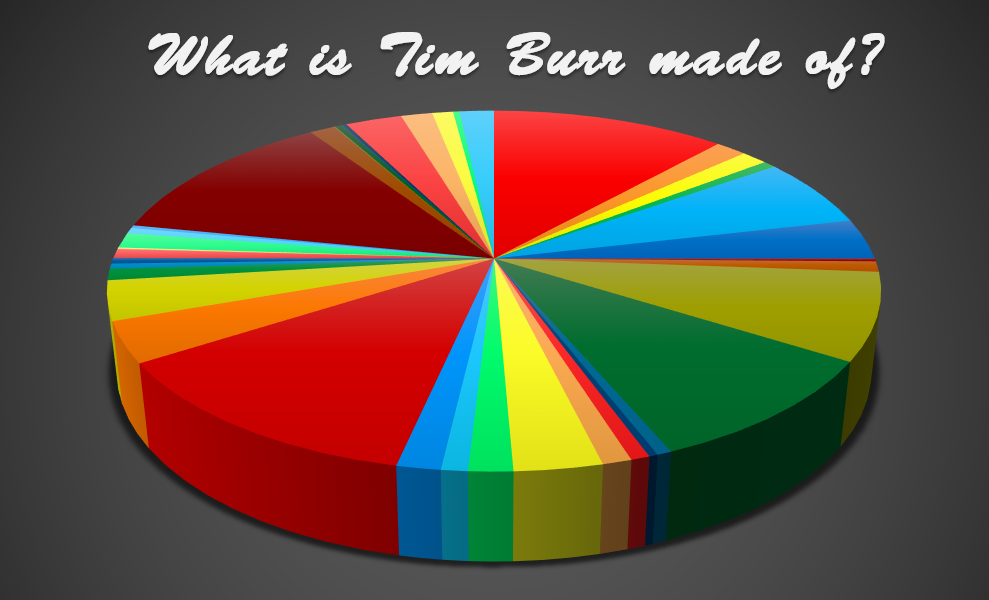
\includegraphics[width=\linewidth]{Images/Main/finance_cover_pic.png}
\end{minipage}

% \addcontentsline{toc}{section}{\numberline{}Mission Statement}
% \subsection*{\textbf{\Huge Mission Statement:}}
% \vspace{.2cm}
% %\begin{flushleft}
% \setlength{\parindent}{.25in} 
% % guidelines http://www.firstinspires.org/sites/default/files/uploads/resource_library/ftc/2016-2017-season/engineering-notebook-guidelines.pdf
% % starts at bottom of page 12

% \large{Our mission is...}
% \newline 
% \hl{Encourage STEM and the FIRST principles in the team and the community to develop the next generation of thinkers, creators and innovators. We do this through our commitment to the transformative power of our STEM-oriented outreach program.}

% \addcontentsline{toc}{section}{\numberline{}Team Overview}
% \subsection*{\textbf{\Huge Team Overview:}}
% \vspace{.2cm}
% \setlength{\parindent}{.25in} 

% \textbf{\Large Mechromancers Team Summary}

% \begin{itemize}
%  \item \textbf{Who are we:} We are Mechromancers, FTC Team 4717, a high school robotics team based in Oviedo, Florida. We operate through the Hagerty Robotics Program at Hagerty High School in Seminole County, along with our sister team 4227 Metal Morphosis.
%  \item \textbf{Team Members:}  We are comprised of fifteen members - eleven boys and four girls - ranging from freshmen to seniors. We are fortunate to have seasoned members who help to guide our newer members. Prospective members are encouraged to attend Hagerty Robotics summer camp to learn more about FIRST’s FTC program and to get hands on experience with robotics before they decide to join the team. 
%  \item \textbf{Team Mentors:} Our team has seven mentors, five of which come from a STEM background. We also have two peer mentors who recently graduated from FTC and now attend The University of Central Florida. The diversity of our mentors makes them great assets to providing training and guidance for the team. Two were previous FIRST members, we also have \hl{skilled professionals like Mr. Harper to assist our team, a machinist and the director of UCF's TI Innovation Lab, a workspace and machine shop,} which the team uses frequently for their builds.
% \end{itemize}

% \textbf{\Large Mechromancers Team History}

% \begin{itemize}
% \item \textbf{Beginnings:}  Mechromancers was originally founded in 2011 as an \textbf{all-female team} known as Estrogenius.  Over the years, the team has evolved and is now known as the Mechromancers.
% \item \textbf{Recent History:}Last year, the Mechromancers’ hard work and dedication paid off as they progressed through the FTC ranks. They were very successful and were on the \hl{Semi Finalist Alliance at the FTC World Championships in Houston, Texas.} Their awards for the 2017-18 Relic Recovery season include:
% \textit{Space Coast League Championship: 1st place Inspire, 3rd place Think Award, 3rd place Control Award, 3rd place PTC Design Award, 3rd place Rockwell Collins Innovate Award, Championship Finalists.State Championship: 1st place Inspire Award. South Super Regional Championship: 1st place Rockewell Collins Innovate Award, 3rd Control Award. World Championship: 1st place Design Award, Compass Award Finalist, Franklin Division Semi-Finalist Captain.}
% \end{itemize}

% \clearpage
% \addcontentsline{toc}{section}{\numberline{}Team Impact}
% \subsection*{\textbf{\Huge Team Impact:}}
% \vspace{.2cm}
% \setlength{\parindent}{.25in} 

% \textbf{\Large Mechromancers Outreach Activities and Events:}

% \textbf{Current Season Outreach:} We love to promote FIRST by \hl{inspiring and connecting with our community.} For our outreach this year, we wanted to focus on \hl{making connections with our community, local stem officials, and our team.} To accomplish this, we went to a Ronald McDonald House to teach kids about science, technology, and our program. We took part in UCF STEM day, where we demoed to young kids our previous season robot Woody, and introduced them our less complicated EV3 robots in order to inspire them to follow STEM programs. We partner with Girl Scout Troop 1649 to assist them with their FLL Junior competition.  We are also excited to connect with local STEM professionals and organizations at engineering conventions and events, such as the Orlando Maker Faire, the Barnes and Noble mini-Maker Faire, and I/ITSEC, the world’s largest modeling, simulation, and training event. 


% \textbf{Plans for Future Outreach:} We are excited about our Outreach opportunities for the remainder of the season, as our calendar is filling up quickly! Our next Outreach event will be demoing our robot and connecting with families at \hl{The Ronald McDonald House} each month throughout the season. 


% \addcontentsline{toc}{section}{\numberline{}SWOT Analysis}
% \subsection*{\textbf{\Huge SWOT Analysis:}}
% \vspace{.2cm}
% %\begin{flushleft}
% \setlength{\parindent}{.25in} 

% \textbf{Analysis of Strengths, Weaknesses, Opportunities, Threats:}
% \vspace{.2cm}
% \textbf{Strengths:} 
% \begin{itemize}
% \item \textbf{Diverse group of students} - bring a variety of backgrounds and interests to the team
% \item \textbf{Extensive Use of CAD} - Almost all parts of the robot were created in the Creo CAD software and built from raw materials. In Creo, movements are simulated using articulating joints, family tables are used to create libraries of similar parts, skeletons used for the top-down design, also all models are fully parameterized.
% \item \textbf{Organization} - We decided to keep our team organized through job specialization, breaking up into committees for each aspect of our team. This allows us to work in parallel while still working together as a team. We use a project management app called Trello as well as Band to help our team communicate.  
% \item \textbf{Custom Parts} - We used 3D printing as well as the laser cutter and machine shop at the University of Central Florida's Innovation Lab to create custom parts for the robot. We work with the director of the lab, Mr. Harper, who is a mentor for the team. 
% \item \textbf{Source Code Control} - We use Github to easily edit and share the code between programmers. This also allows us to track changes in the code and fix past errors.
% \item \textbf{Use of \LaTeX} - used \LaTeX typesetting language and Overleaf.com to create an engineering notebook that can be easily edited and formatted.
% \end{itemize}

% \textbf{Weaknesses:} 
% \begin{itemize}
% \item Large Team - it can be hard to come to a consensus when a decision needs to be made.
% \item Creo and Programming Knowledge - While the team is working to train new members in CAD and Programming, we currently only have a few students who are fully trained.
% \end{itemize}

% 	\textbf{Opportunities:} 
% \begin{itemize}
% \item Location - there are a \textbf{large number of STEM based organizations in Central Florida that we could reach out to for additional mentorship}
% \item Promote FIRST - expansion of our Outreach program to include more \textbf{mentoring of youth either through after-school or summer camp opportunities}
% \end{itemize}

% 	\textbf{Threats}
% \begin{itemize}
%  \item Loss of sponsors/grants - would make it hard for our team to financially support itself
%  \item Graduating seniors - losing team cohesion due to graduation of members
% \end{itemize}

% \textbf{\Large Action Plan:}

% \textbf{Expand Outreach Opportunities:} Reach out to additional schools in Seminole County to provide \hl{mentorship for current robotics clubs/FLL teams} and push to start an after-school robotics club at our local elementary school.

% \textbf{Focused Technical Training:} Continue to provide \textbf{technical training in areas such as PTC Creo and Programming} during the FTC season and offer specialized training with current and/or new mentors during the off-season/over the summer with the goal of \textbf{encouraging all members to become familiar with both CAD and Programming.}

% \textbf{Engage Local STEM Community:} Look for additional opportunities to \hl{connect with local STEM professionals} to add to our already amazing pool of volunteer mentors in order to ensure the team \textbf{has access to some of the best minds in the business.}

% \textbf{Strengthen Sponsorship Connections:} Create (and stick to) a process to better engage our current and future sponsors throughout the FTC season and provide timely updates on the team’s progress to not only thank sponsors for their generosity, but to share our enthusiasm for FIRST with them.

% \subsection*{\textbf{\Huge Sustainability}}
% % This plan explains how the Team plans to grow and stay competitive when students graduate from the program. This may include plans to recruit sponsors,new Mentors, or Team members.

% In order to ensure that our team \textbf{retains its competitive edge} we have a variety of strategies we use to train new members. For example, every year we host a \hl{\textbf{summer camp} for incoming members to participate in.} This camp gives incoming members a taste of FIRST, and over the course of the camp, teams of students build and design robots to compete on the third day! We also have a notebook challenge, because the engineering notebook is an important part of the competition. This is a laid-back, fun camp where students can learn  values and skills to use during the season. Additionally, we have created several \hl{\textbf{committees within our team that graduating members lead}}. This allows the graduating members to \textbf{pass down all the techniques, skills, and information they have learned over their past participating years to the less experienced members}. This helps to ensure that we are constantly growing as a team and improving our problem solving abilities. Additionally, at the end of each year we \hl{\textbf{send personalized thank you letters} to each of our sponsors to maintain a strong relationship with them.} In these letters we included the season's successes and achievements to demonstrate what we were able to achieve with their help. You can see a list of our sponsors along with their donations in Table \ref{sponsors}. 

% \addcontentsline{toc}{section}{\numberline{}Financial Goals and Sponsors}
% \subsection*{\textbf{\Huge Financial Goals and Sponsors:}}
% \vspace{.2cm}
% %\begin{flushleft}
% \setlength{\parindent}{.25in} 
% % guidelines http://www.firstinspires.org/sites/default/files/uploads/resource_library/ftc/2016-2017-season/engineering-notebook-guidelines.pdf
% % starts at bottom of page 12

% To ensure we can provide the funds necessary to cover our team's expenditures, we have set many financial goals. \hl{Collectively, we strive to accumulate \textbf{\$5,000} during the 2018-2019 season} to provide the necessary funds to support our team.  We accomplish this goal by obtaining \$150 from each member, \hl{requiring each member to obtain \$100 in donations or sponsorships,} and by participating in several fundraising events such as spirit nights. The money we acquire will go towards paying for the goals we have listed below:

% \begin{itemize}
%   \item \textbf{\Large Travel Goal: \$3,000 }
%   \newline 
%   Whenever we stay overnight at hotels or travel out of state for a competition, we incur additional expenses like paying for gas, meals, and hotel rooms. Most of these expenses will be \hl{paid by team members} as part of the travel fee they must pay in order to go to the competition. We estimate that the total cost of travel to the State, and World Championships will be \$3,000, so \hl{throughout the competition season we will be charging students travel fees ranging from \$50 to \$400 if we advance.}
  
%   \textbf{Current Progress: }
%   For the closer events we have participated in that are only 1 hour away, we require members to provide their own transportation; however, we encourage carpooling. For events such as States and Worlds we \hl{provide vans and hotel rooms for the participating members and split the total fees among all participating members.} We require members to pay for themselves to participate in these events due to the high price tags. Our financial income, consisting of donations and sponsorships, do not cover all of these costs. Therefore, we do our best each year to gain more sponsors for our team in hopes that we will be able to one day pay for these costs. To ensure we keep our sponsors happy to donate to our team each year, we \textbf{send them a final update on the seasons events along with a thank you letter for all of their help and encouragement.} 
% %%%%%%%%%
%   \item \textbf{\Large Competition Field Goal: \$258}
%   \newline 
%    The field in total costs \$480.00. However, this cost is split between our team and our sister team since we will both have full time access to the field. We thought that the field was an extremely important asset to take into account with our finances. The field allows us to practice our autonomous program and teleop driving skills. \hl{Our performance on the field during competition is 50\% of our overall score.} Therefore, being able to accurately practice and perfect our skills allows us to perform better during the matches. In order to meet this goal we will use the money we have accumulated \textbf{from fundraising} for our team.
%   \newline 
% \textbf{Current Progress:} We have purchased a practice field for our team to use. This has been a very valuable asset to our team. We have used the field almost everyday and invited the Plaid Piranhas to come to Hagerty to assist them with their arm this season.
% %%%%%%%%%  
%   \item \textbf{\Large Competition Fee Goal: \$1,450}
%   \newline 
%   The entry fee for each competition increases with the advancement through the championships. Typically, registration for league meets costs \$60, the state championship costs \$150, and World's costs \$1,000. Therefore, our goal is \textbf{representative of the registration fees} for the 3 league competitions we participated in.
  
%   %\newline 
%   \textbf{Current Progress: }
%  	Thus far into the season we have been able to pay for all of our league events from our team account. As we progress through competition levels we use the money we received from our sponsors to help pay the registration costs. Therefore, in order to ensure this money to our team we always send thank you notes with a list of our accomplishments to our sponsors. We truly appreciate their donations and encouragement they provide us with season after season. 
% %%%%%%%%%
%   \item \textbf{\Large Hardware Goal: \$500 }
%   \newline 
%   Since we have competed in previous seasons, we can reuse parts from our older robot designs in our current robot. This reduces the overall cost of the new hardware we would need to purchase. 
%   \newline
%   \textbf{Current Progress: }
%   This goal is a priority for us to meet since our robot, Bullseye, is the center of our team. Therefore, our income is first used towards paying for our various hardware expenses. Our income consists of the money we obtain \textbf{from membership dues, donations, and sponsorships}. As one can see from Table \ref{my-label} our robot currently costs \hl{\$1247.50.} We have accumulated many of these pieces from previous robot designs meaning that this is not the cost we had to pay for this years new hardware. This season's new hardware cost us a total of \hl{\$334.11}. This means that we set a higher goal than we needed to achieve. This is a good sign for us meaning that we were ready to anticipate spending more money than we needed to. The left over money that we would have contributed to hardware can now be distributed to other areas of financial need such as our Competition fee goals, saved for the future, and hardware needs for the season.
% %%%%%%%%%
%   \item \textbf{\Large Fundraising Goal: \$5,000 }
%   \newline 
% In the beginning of the season we set a goal for each member to raise \$100 to help support our team. Since we have 15 members on our team we initially set our fundraising goal to \$1,500. However, throughout the year we have \hl{gone to several fundraising events including spirit nights and the Mini Maker Faire, in which we accepted donations for our team expenditures.} Additionally, with the help of our long time sponsors, such as Lockheed Martin and DoD STEM. Since we have been able to meet our fundraising goals, we increased our goal to \$5,000. 
%   \newline 
%   \textbf{Current Progress: }We have accepted several donations from family members of the team as well as local businesses. Chick-fil-A was one of our fundraising where we achieved over \$150. Another fundraising event we did was over the summer known as Robo-boat, where it was a smaller competition where we had a team make a boat to compete in a fully autonomous race. Our team made it to second place, bringing in \$2,000 for our team. More about this specific accomplishment can be found in the outreach section of our notebook. In total we have accumulated \hl{\$7406.69 of sponsorships and donations}. This means that we have surpassed our fundraising goal for this year!
  
% \end{itemize}

% Even though these goals accumulate to \$3,000 more than our overall team goal of \$5,000, this goal represents the realistic costs our fundraising activities can provide for us. As previously mentioned, we do not expect our team to be responsible for meeting all of the ideal goals involving travel fees. We feel that since not everyone can participate in each event, then the money we raise as a team should go towards things all team members can enjoy such as our robot. In doing so, we are able to account for this extra amount of money that we as a team are not able to raise. We do, however, do our best to ensure a fair and even spread of our team finances. By this, we mean to say that surplus money we raise past our fundraising goal does go to lowering the overall cost members who travel pay. This money goes towards buying vans for transportation purposes. 

% \begin{table}[ht!]
% \tiny
% \centering
% % \caption{Our Robot (Bullseye) Costs}
% \label{my-label}
% \begin{tabular}{
% >{\columncolor[HTML]{77E1FF}}l 
% >{\columncolor[HTML]{D1E5EA}}l 
% >{\columncolor[HTML]{77E1FF}}l 
% >{\columncolor[HTML]{D1E5EA}}l 
% >{\columncolor[HTML]{77E1FF}}l }
% %\hline
% \cellcolor[HTML]{3DD0F9}Robot Materials & \cellcolor[HTML]{B7CFD6}Description    & \cellcolor[HTML]{3DD0F9}Quantity & \cellcolor[HTML]{B7CFD6}Unit Price & \cellcolor[HTML]{3DD0F9}TOTAL               \\ %\hline
% Medium Density Fiberboard               & Wood Used on Robot                     & 4                                & \$7.49                             & \$29.96                                     \\
% VEX Pro 1/2" Hex Shaft                  & Connects Supporter Arms                & 2                                & \$10.00                            & \$20.00                                     \\ 
% \#25 Chains/Links                       &  Standard Textrix Chain                & 2                                & \$13.95                            & \$27.90                                     \\
% Nyon-Spandex Blend                      & Used to Shoot the Minerals             & 1                                & \$10.00                            & \$10.00                                     \\
% Andy Mark Motors                        & Arm Motors and Winch                   & 4                                & \$24.95                            & \$99.80                                     \\
% Tetrix 40:1 Motors                      & Drive Train Motors                     & 2                                & \$10.00                            & \$20.00                                     \\
% REV Core HEX Motors                     & Shooter Motor                          & 1                                & \$21.00                            & \$21.00                                     \\
% On-Off Switch                           & Turn the Robot On and Off              & 1                                & \$12.95                            & \$12.95                                     \\
% OTG Cables                              & Cables for Modules                     & 6                                & \$3.00                             & \$18.00                                     \\
% USB Cables                              & Cables for Modules                     & 6                                & \$5.00                             & \$30.00                                     \\
% REV Robotics Expansion Hub              & Talks to Motors                        & 2                                & \$79.95                            & \$159.90                                    \\
% 0.25" Steel Axles                       & For All Rotating Parts                 & 1                                & \$1.50                             & \$1.50                                      \\
% Standoff                                & Used to on Shooter Lever               & 1                                & \$0.50                             & \$0.50                                      \\
% Spacers                                 & Axle Spacers                           & 24                               & \$0.05                             & \$1.20                                      \\
% 6-32 Screws                             & Connect Parts                          & 47                               & \$0.03                             & \$1.41                                      \\
% ServoCity Servo Motors                  & Hang arm                               & 10                               & \$12.99                            & \$129.90                                    \\
% Phone                                   & Communicate to Robot                   & 2                                & \$120.00                           & \$240.00                                    \\
% Nuts                                    & Hold screws                            & 42                               & \$0.03                             & \$1.37                                      \\
% Hall Effect Sensor                      & Used to Detect Arms                    & 1                                & \$25.00                            & \$25.00                                     \\
% VEX motors                             & Intake Motor                            & 1                                & \$ 14.99                            &\$14.99                                      \\
% VEX Chain and Sprockets                & Standard Vex Chain and Sprockets        & 1                                & \$
% 12.99                            &\$12.99                                      \\
% 1/8" Piano Wire                        & Used for the Hang Hook                  & 1                                & \$
% 10.48                            &\$10.48                                      \\
% Touch Sensor                           & Auto Initialization Efficiency          & 2                                & \$
% 6.00                             &\$12.00                                      \\
% 20lb Aluminium Stock                   & Big Wheel Hubs                          & 1                                & \$
% 40.00                            &\$40.00                                      \\
% Tetrix Gear Kit                        & Gear the Big Wheel Drive                & 2                                & \$
% 17.95                            &\$35.90                                      \\
% 8mm Shafts                             & Axles on Big Wheel Drive                & 2                                & \$
% 12.95                            &\$29.50                                      \\
% One way bearing                        & Bearing on Drivetrain Axles             & 1                                & \$
% 12.50                            &\$12.50                                      \\ 
% VEXPRO 1/2" Radial Bearings            & Used on the Arms                        & 4                                & \$
% 4.99                             &\$19.96                                      \\
% VEXPRO 32 Teeth Sprockets              & To Activate the Arms                    & 2                                & \$
% 13.99                            &\$27.98                                      \\
% VEXPRO 16 Teeth Sprockets              & To Activate the Arms                    & 2                                & \$
% 7.99                             &\$15.98                                      \\
% XL Timing belts                        & Used on Conveyor                        & 4                                & \$
% 5.27                             &\$21.08                                      \\
% Targus Hub                             & Used for Phone                          & 1                                & \$
% 46.99                            &\$46.99                                      \\
% REV Servo Power Module                 & Power the Servos                        & 1                                & \$
% 40.00                            &\$40.00                                      \\
% VEXPRO D-Shaft Clamping Hub            & Hold on Sprocket for Arm                & 2                                & \$
% 4.99                             &\$10.00                                      \\
% Tetrix 144mm angle                     & Used on Shooter Mount                   & 1                                & \$
% 10.95                            &\$10.95                                      \\
% Lexan Sheet                            & Used for doors on wheel                 & 1                                & \$
% 24.86                            &\$24.86                                      \\

% \cellcolor[HTML]{34FF34}\textbf{TOTAL:} & \cellcolor[HTML]{34FF34}               & \cellcolor[HTML]{34FF34}258      & \cellcolor[HTML]{34FF34}           & \cellcolor[HTML]{34FF34}\textbf{\$1247.50} \\ %\hline
% \end{tabular}
% \end{table}

% \clearpage

% \begin{table}[ht!]
% \centering
% % \caption{Sponsorships and Donations}
% \label{sponsors}
% \begin{tabular}{ 
% >{\columncolor[HTML]{77E1FF}}l 
% >{\columncolor[HTML]{D1E5EA}}l 
% >{\columncolor[HTML]{77E1FF}}l 
% >{\columncolor[HTML]{D1E5EA}}l}
% % \hline
% \cellcolor[HTML]{3DD0F9}Contributor & \cellcolor[HTML]{B7CFD6}Contribution    &\cellcolor[HTML]{3DD0F9}Contributor & \cellcolor[HTML]{B7CFD6}Contribution    \\ %\hline
% Chik-fil-A              & \$55          &   National Center for STEM& \$325          \\
% Publix                  & \$224.67      &   Verizon                 & \$375          \\
% Lockheed Martin         & \$1500        &   DoD STEM                & \$1000         \\
% SCPS                    & \$250         &   Rockwell Collins        & \$250          \\
% Engineering Consultants & \$100         &   SIEMENS                 & \$750          \\
% Barnes and Noble        & In Kind       &   GES                     & \$177.03       \\
% Winn Dixie              & In Kind       &   Klages Kreations        & In kind        \\
% NCASE                   & \$216.66      &   Actobotics              & \$200          \\
% AUVSI                   & \$1333.33     &   AKT                     & \$100          \\
% Chen Family             & \$100         &   Dickison Family         & \$100          \\
% Guise Family            & \$100         &   Miller Family           & \$250          \\


                                        
% \cellcolor[HTML]{34FF34}\textbf{TOTAL: \$7406.69 1} & \cellcolor[HTML]{34FF34} & \cellcolor[HTML]{34FF34} & \cellcolor[HTML]{34FF34} \\ %\hline
% \end{tabular}
% \end{table}

% \begin{figure}[ht!]
% \centering
%   \caption{Here's Some Cool Sponsor Logos}
%   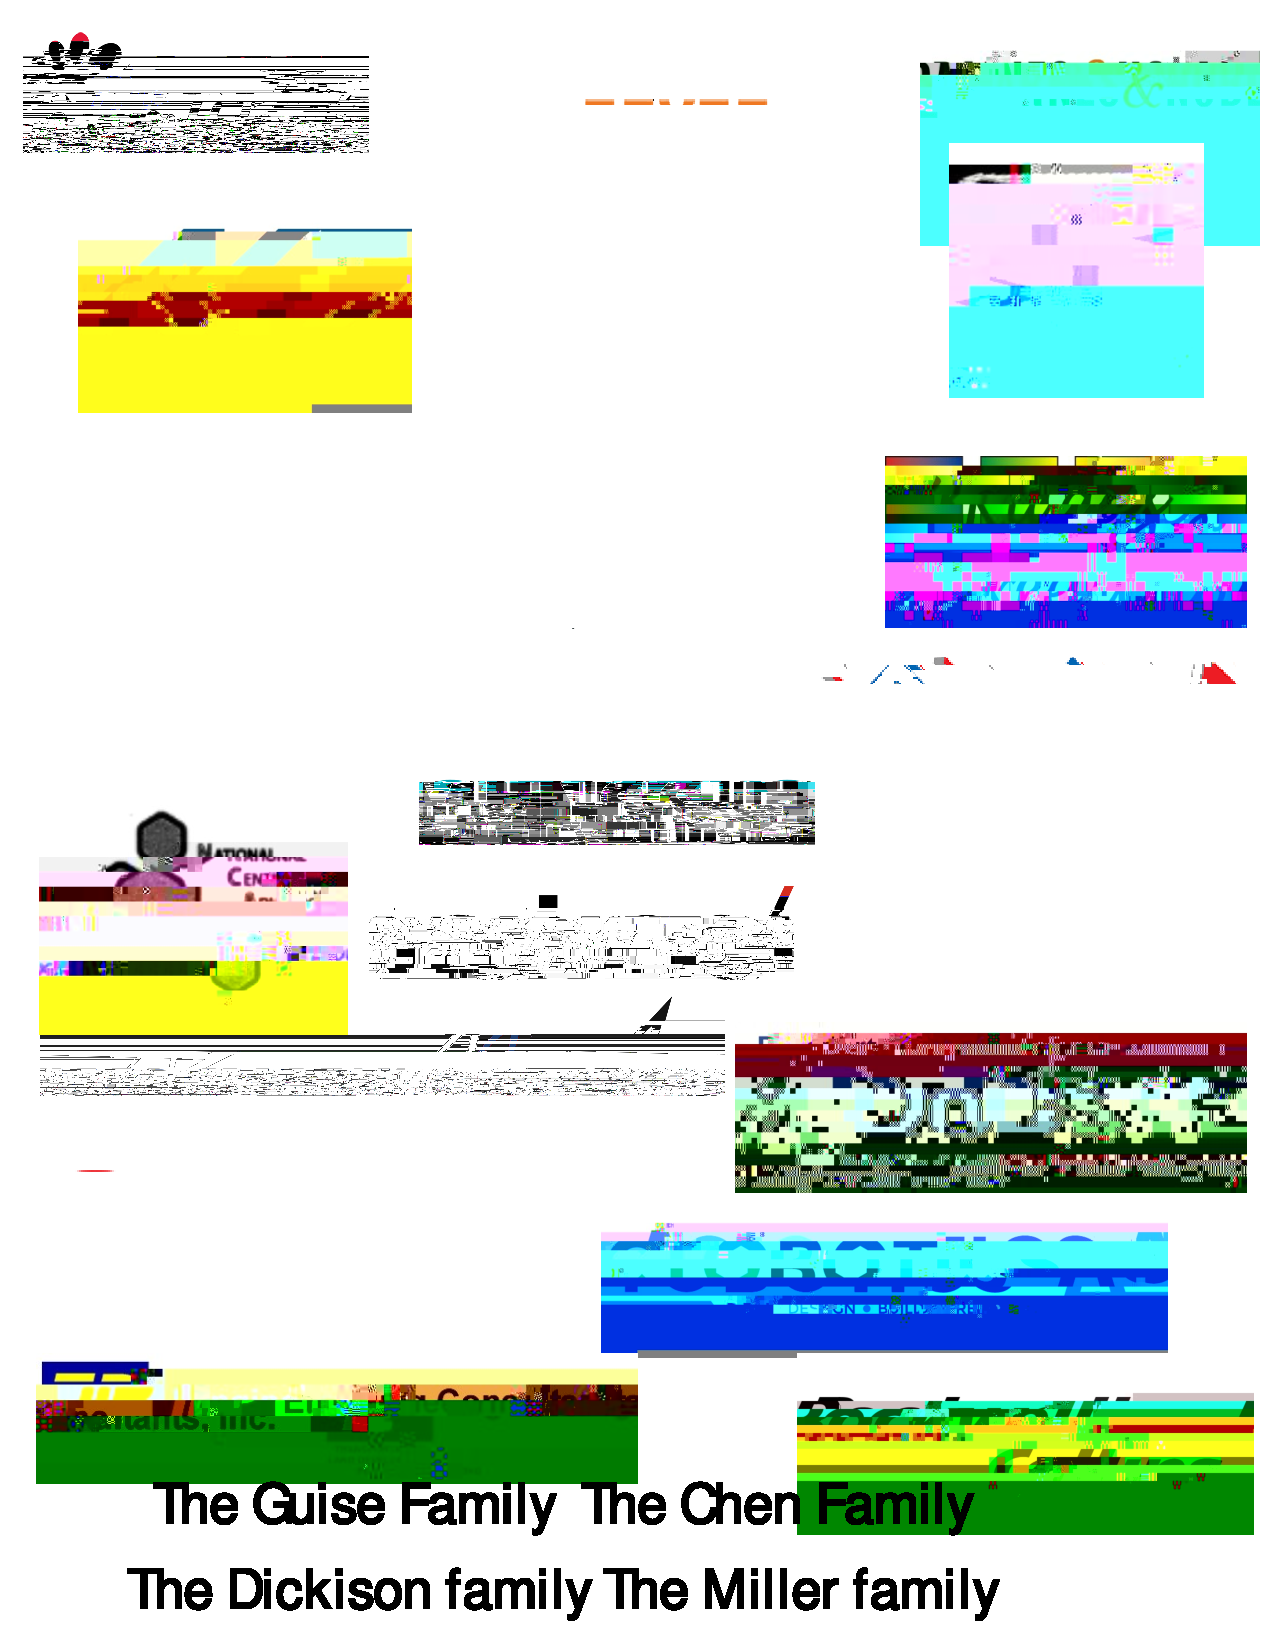
\includegraphics[width=0.9\linewidth]{Business/Images/Sponsors.pdf}
%   %\label{fig:Sponsors}
% \end{figure}

% \clearpage 







%%%%%%%%%%%%%%%%%%%%%%%%%%%%%%%%%%%% Here we can add sponsors logos %%%%%%%%%%%%%%%%%%%%%%%%%%%%%%%%%%%%%


%%%%%%%%%%%%%%%%%%%%%%%%%%%%%%%%%%%%%%%%%%%%%%%%%%%%%%%%%%%%%%%%%%%%%%%%%%%%%%%%%%%%%%%%%%%%%%%%%%%%%%%%%%%

% \begin{flushleft}
% \subsection*{\textbf{\Large This is a complete list of our sponsors:}}
% \begin{tabular}{ p{5cm} p{5cm} }
% 	\begin{itemize} 
%     \item DHA and Calpec 
%     \item Unical Aviation Inc.
%     \item Oviedo Woman's  
%     \item Ferber Family
%     \item Garcia Family
%     \item Mason Family
%     \item Ruplinger Family
%     \item Marco's Pizza
%     \item Duckin' Donuts
%     \item Tijuana Flats
%     \item Siemens 
%     \end{itemize}
    
%     & 
    
%     \begin{itemize} 
%     \item Lockheed Martin 
%     \item TLP Engineering
%     \item Gnan Engineering
%     \item Chen Family
%     \item Dishman Family
%     \item Freece Family
%     \item Chick-fil-A
%     \item Beef'O'Brady's
%     \item Actobotics
%     \item Disti
%     \item NAWC
%     \end{itemize} \\
    
% \end{tabular}
% \end{flushleft}


% % Please add the following required packages to your document preamble:
% % \usepackage{graphicx}
% % \usepackage[table,xcdraw]{xcolor}
% % If you use beamer only pass "xcolor=table" option, i.e. \documentclass[xcolor=table]{beamer}
% \begin{table}[]
% \caption{My caption}
% \label{my-label}
% \resizebox{\textwidth}{!}{%
% \begin{tabular}{
% >{\columncolor[HTML]{77E1FF}}l 
% >{\columncolor[HTML]{D1E5EA}}l 
% >{\columncolor[HTML]{77E1FF}}l 
% >{\columncolor[HTML]{D1E5EA}}l 
% >{\columncolor[HTML]{77E1FF}}l }
% \hline
% \cellcolor[HTML]{3DD0F9}Robot Materials & \cellcolor[HTML]{B7CFD6}Description    & \cellcolor[HTML]{3DD0F9}Quantity & \cellcolor[HTML]{B7CFD6}Unit Price & \cellcolor[HTML]{3DD0F9}TOTAL               \\ \hline
% Sprocket                                & Transfer Motor Rotation                & 14                               & \$15.95                            & \$223.30                                    \\
% Bevel Gear                              & Transfer Motor Rotation 90°            & 2                                & \$15.00                            & \$30.00                                     \\
% Aluminum Poles                          & Holds Drive Train Sides Together       & 5                                & \$5.00                             & \$25.00                                     \\
% VEX Green Gear                          & Utilized for Whisker Sensors           & 4                                & \$3.00                             & \$12.00                                     \\
% 3D Printed Shooter Wheels               & Used to Shoot Particles                & 2                                & \$60.00                            & \$120.00                                    \\
% \#25 Chains/Loops                       & Standard Textrix Chains                & 5                                & \$13.95                            & \$69.75                                     \\
% Sweeper Aluminum Pole                   & Holds Rubber Hose for Sweeper          & 1                                & \$5.00                             & \$5.00                                      \\
% Automotive Rubber Hose from Autozone    & Used to Sweep Balls                    & 3                                & \$6.00                             & \$18.00                                     \\
% Andy Mark Motors                        & Sweeper and Shooter Motors             & 6                                & \$24.95                            & \$149.70                                    \\
% Bane Bot 20:1 Planetary Gear Boxes      & Drive Train Motors                     & 4                                & \$46.50                            & \$186.00                                    \\
% VEX Motors                              & Inner Sweeper and Button Pusher        & 2                                & \$4.95                             & \$9.90                                      \\
% VEX Conveyor Belt Flaps                 & Used to Feed Particles                 & 6                                & \$1.00                             & \$6.00                                      \\
% On-Off Switch                           & Turn the Robot On and Off              & 1                                & \$12.95                            & \$12.95                                     \\
% Tetrix Channels                         & Hold Phone and Sweeper                 & 2                                & \$9.95                             & \$19.90                                     \\
% Shooter Wheel Plates                    & CNC Aluminum Motor Plates              & 2                                & \$30.00                            & \$60.00                                     \\
% Medium Density Fiberboard               & Wood used on Robot                     & 4                                & \$7.50                             & \$30.00                                     \\
% OTG Cables                              & Cables for Modules                     & 6                                & \$3.00                             & \$18.00                                     \\
% USB Cables                              & Cables for Modules                     & 6                                & \$5.00                             & \$30.00                                     \\
% MR Core Motor Controller                & Talks to Motors                        & 3                                & \$79.95                            & \$239.85                                    \\
% MR Core Servo Controller                & Talks to Servos                        & 1                                & \$69.95                            & \$69.95                                     \\
% MR Device Interface Module              & Sensor Module                          & 1                                & \$67.95                            & \$67.95                                     \\
% Steel Axles                             & For All Rotating Parts                 & 13                               & \$1.50                             & \$19.50                                     \\
% Standoff                                & Used to Hold Plates Apart              & 18                               & \$0.50                             & \$9.00                                      \\
% Tetrix Flat Bar                         & Whisker Arm                            & 1                                & \$9.95                             & \$9.95                                      \\
% VEX Bracket                             & Connects Rack and Pinion Assembly      & 4                                & \$3.95                             & \$15.80                                     \\
% Spacers                                 & Axle Spacers                           & 24                               & \$0.05                             & \$1.20                                      \\
% Screws                                  & Connect Parts                          & 47                               & \$0.03                             & \$1.41                                      \\
% Servo Motors                            & Control Arm on Whisker Sensor          & 2                                & \$12.99                            & \$25.98                                     \\
% Velcro Straps                           & Hold Down Shooter Assembly             & 2                                & \$5.00                             & \$10.00                                     \\
% Acrylic Plates                          & Connect all Modules to                 & 1                                & \$5.00                             & \$5.00                                      \\
% Phone                                   & Communicate to Robot                   & 2                                & \$120.00                           & \$240.00                                    \\
% Carbon Fiber Tubes                      & Housing for Particles and Scissor Lift & 6                                & \$4.00                             & \$24.00                                     \\
% Nuts                                    & Hold Screws                            & 42                               & \$0.03                             & \$1.37                                      \\
% VEX Racks                               & Racks for Button Pusher                & 3                                & \$2.00                             & \$6.00                                      \\
% VEX Rail                                & Mount for Rack and Pinion              & 1                                & \$1.50                             & \$1.50                                      \\
% Optical Distance Sensor                 & Used to Detect White Lines             & 2                                & \$26.95                            & \$53.90                                     \\
% Wheels                                  & For Drive Train                        & 6                                & \$4.99                             & \$29.94                                     \\
% Potentiometers                          & Used on Whisker Sensors                & 2                                & \$10.00                            & \$20.00                                     \\
% AdaFruit Color Sensor                   & Detect Color on Beacons                & 1                                & \$5.95                             & \$5.95                                      \\
% MR Gyro Sensor                          & Used to find Current Heading           & 1                                & \$32.95                            & \$32.95                                     \\
%                                         &                                        &                                  &                                    &                                             \\
% \cellcolor[HTML]{34FF34}\textbf{TOTAL:} & \cellcolor[HTML]{34FF34}               & \cellcolor[HTML]{34FF34}258      & \cellcolor[HTML]{34FF34}           & \cellcolor[HTML]{34FF34}\textbf{\$1,916.70} \\ \hline
% \end{tabular}%
% }
% \end{table}

% Please add the following required packages to your document preamble:
% \usepackage[table,xcdraw]{xcolor}
% If you use beamer only pass "xcolor=table" option, i.e. \documentclass[xcolor=table]{beamer}





\financemodule
{We do money things}
{Business/Images/Expenses_Chart_1.png}
{hi}
{Business/Images/Expenses_Chart_1.png}
{hiz}
{Business/Images/Expenses_Chart_1.png}
{hic}
{Business/Images/Expenses_Chart_1.png}
{hiv}


                  

 %           ______             _                      _               _____           _            
 %          |  ____|           (_)                    (_)             |  __ \         | |           
 %  ______  | |__   _ __   __ _ _ _ __   ___  ___ _ __ _ _ __   __ _  | |__) |_ _ _ __| |_   ______ 
 % |______| |  __| | '_ \ / _` | | '_ \ / _ \/ _ \ '__| | '_ \ / _` | |  ___/ _` | '__| __| |______|
 %          | |____| | | | (_| | | | | |  __/  __/ |  | | | | | (_| | | |  | (_| | |  | |_          
 %          |______|_| |_|\__, |_|_| |_|\___|\___|_|  |_|_| |_|\__, | |_|   \__,_|_|   \__|         
 %                         __/ |                                __/ |                               
 %                        |___/                                |___/  

\cleardoublepage
\part{Engineering Section}
\vspace{3em}
\begin{minipage}[c]{\linewidth}
\centering
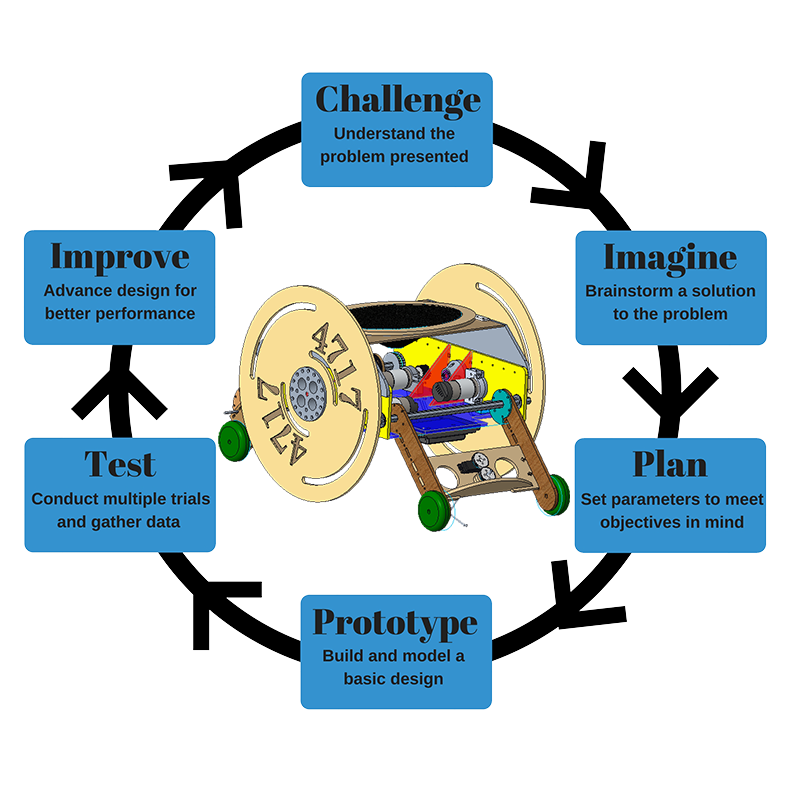
\includegraphics[width=\linewidth]{Images/Main/Challenge.png}
\end{minipage}


 %       __  __           _   _                 
 %      |  \/  |         | | (_)                
 %      | \  / | ___  ___| |_ _ _ __   __ _ ___ 
 %      | |\/| |/ _ \/ _ \ __| | '_ \ / _` / __|
 %      | |  | |  __/  __/ |_| | | | | (_| \__ \
 %      |_|  |_|\___|\___|\__|_|_| |_|\__, |___/
 %                                     __/ |    
 %                                    |___/  

\cleardoublepage
\section{Meetings}
\begin{minipage}[c]{\linewidth}
\centering

\includegraphics[width=\linewidth]{Images/Main/meeting_cover.jpg}
\end{minipage}

% 1) Title
% 2) Date
% 3) Location
% 4) Present
% 5) Picture
% 6) Start Time
% 7) Stop Time
\insertmeeting 
	{Freight Frenzy Kick Off} 
	{09/18/21}
	{Hagerty High School}
	{Jenson}
	{Images/RobotPics/robot.jpg}
	{2:30}
  {4:30}
	
\section*{General}
\noindent\hfil\rule{\textwidth}{.4pt}\hfil
\subsection*{Goals}
\begin{itemize}
    \item Watch kickoff
    \item Brainstorm   

\end{itemize} 

\noindent\hfil\rule{\textwidth}{.4pt}\hfil

\subsection*{Accomplishments}
Today, we watched the kickoff.
 

\begin{figure}[ht]
\centering
\begin{minipage}[b]{.50\textwidth}
  \centering
  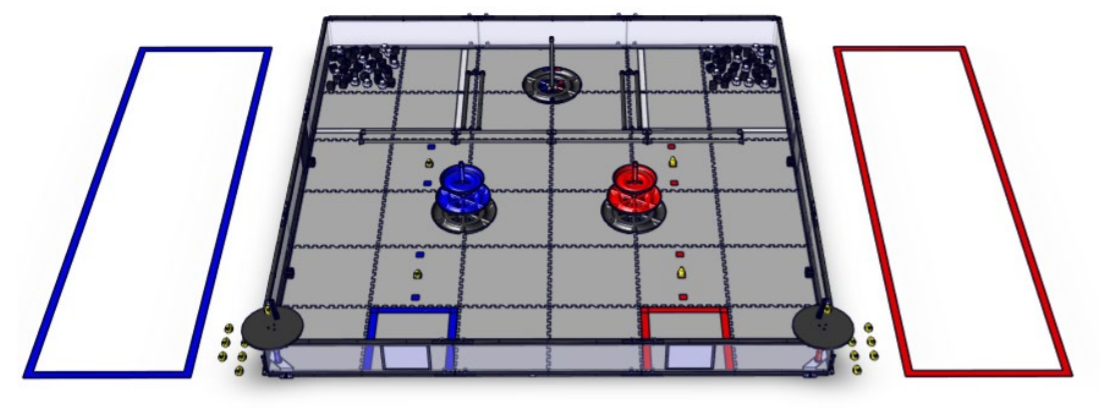
\includegraphics[width=0.8\textwidth]{Meetings/September/09-18-21/field.png}
  \caption{New Account in Github}
  \label{fig:pic1}
\end{minipage}%
\hfill%
\begin{minipage}[b]{.50\textwidth}
  \centering
  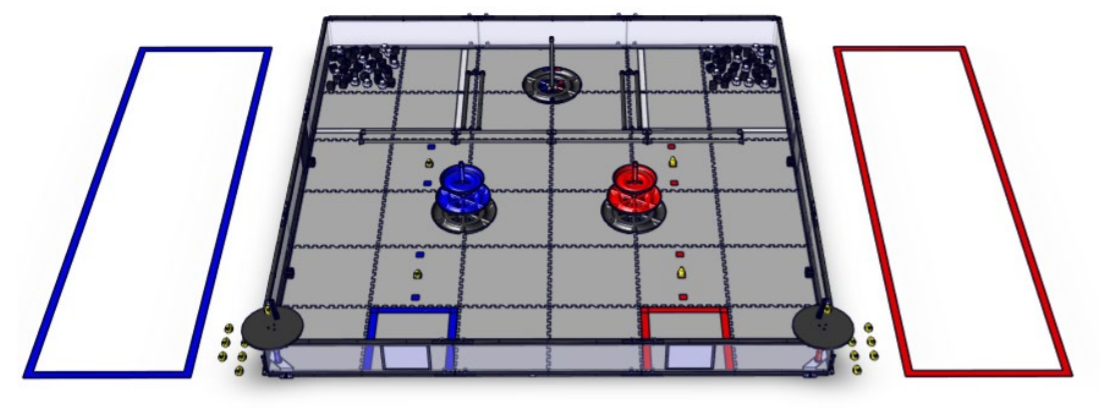
\includegraphics[width=0.8\textwidth]{Meetings/September/09-18-21/field.png}
  \caption{Screenshot of GitHub Repository}
  \label{fig:pic2}
\end{minipage}
\end{figure}








%%%%%%%%%%%%%%%%%%%%%%%%%%%%%%%%%%%%%%%%%%%%%%
%                insertmeeting
% 1) Title (something creative & funny?)
% 2) Date (MM/DD/YYYY)
% 3) Location (ex. Hagerty High School)
% 4) People/Committees Present 
% 5) Picture 
% 6) Start Time & Stop Time (ex. 12:30AM to 4:30PM)
%%%%%%%%%%%%%%%%%%%%%%%%%%%%%%%%%%%%%%%%%%%%%%
\insertmeeting 
	{Star Squad} 
	{09/21/21}
	{Hagerty High School}
	{Clayton, Jensen, Nathan, Ritam}
	{Images/RobotPics/robot.jpg}
	{2:30 - 4:30}
	
\subsection*{Hardware}
\noindent\hfil\rule{\textwidth}{.4pt}\hfil
\subsubsection*{Goals}
\begin{itemize}
    \item Plan and establish what drivetrain we will be building initially.   

\end{itemize} 

\noindent\hfil\rule{\textwidth}{.4pt}\hfil

\subsubsection*{Accomplishments}
During this meeting, the hardware squad met up to discuss the intake. We were between two main ideas, having a six wheeled tank drive with the inner wheels on each side larger than the others. This would allow the robot to wobble and adjust when it first hits the bars it must go over. This could be effective but we thought it might also cause some issues with consistency as the robot would be off center and not have all wheels on the ground. Our next idea was using a similar design to a different team that used 4 separate wobbling mechanisms that will adjust as the robot goes over the bars. This would be helpful as it would be more smooth than just running over the bars but at the same time, we thought it would be better to be more original in our drivetrain and not attempt to copy someone else. Then, all of our ideas changed when Mr. Harper came to rescue us. When Mr. Harper came in, we began by discussing the possibility of using a robot that is less than 13 inches in width. This would allow us to go around the bars and not go over them. This may be efficient because we would not have to worry about losing all of our momentum. On the other hand, it could be hard to build our intake off of a smaller chassis. It would also require us to go a further distance than going straight for the storage unit. We also discussed how our robot needed to be fast in order to be properly efficient. We came to this conclusion because we can only pick up one freight out a time. In order to keep our robot fast, we discussed making our robot lighter which would allow for less weight on the motors and more efficiency. We also discussed changing to using a 10 to 1 gear ratio which would also make the wheels spin faster. Then we discussed a couple of constraints our robot would have like the fact we can only bring one freight at a time, we need to stay light, and we must fully enter the storage area and fully exit it as well. We said to begin with it may be best to do a four wheeled tank drive with side driveplates higher than normal which would allow to possibly go over the bars. It would also make the robot lighter than previous robots that used six wheels. We also decided it would be beneficial for us to test between a larger and a smaller robot because depending on the size, we may have different efficiencies and better strengths and weaknesses when it comes to maneuverability and speed. We know that the motors are between 4.5 to 5.5 inches depending on the brand which means that the motors will take up a lot of space. To negate this use of space there was discussion of placing the motors vertically. Then we finally discussed the intake and how we need to keep it simple. We discussed how we could use some sort of arm to intake the particles. Something we did not take into account when discussing this was the ducks and how we would intake the ducks.

\begin{figure}[htp]
\centering
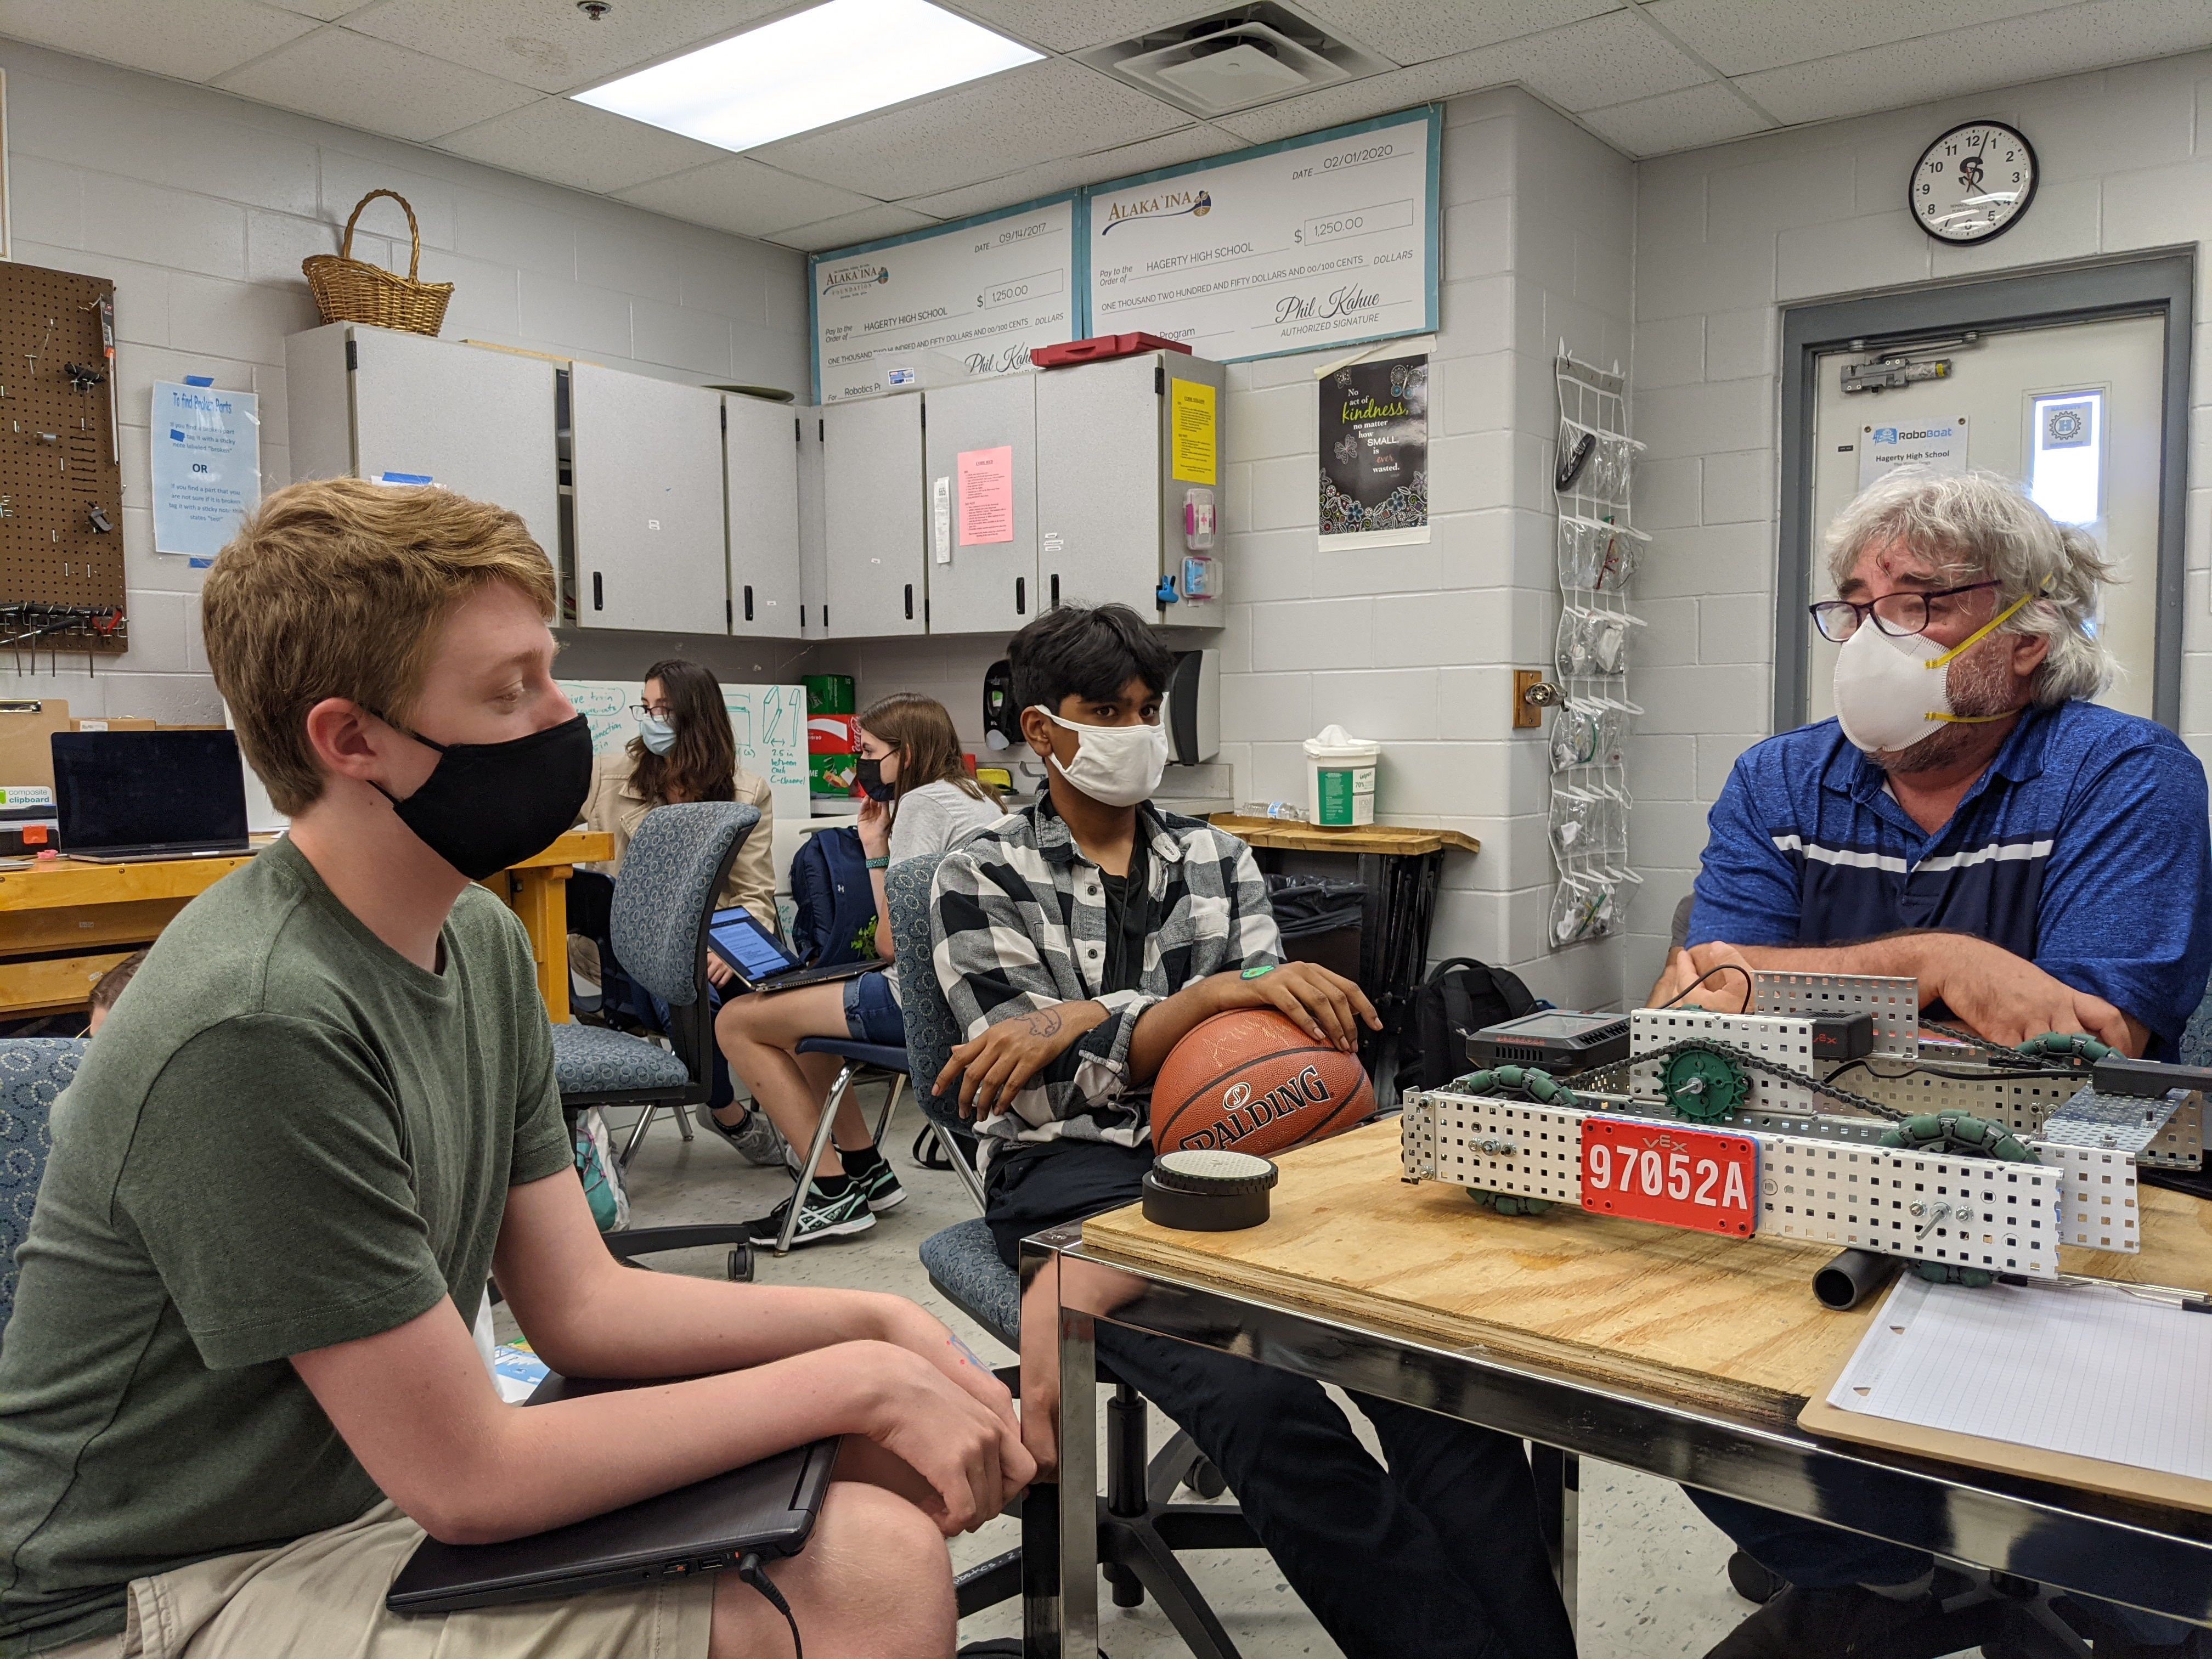
\includegraphics[width=0.9\textwidth, angle=0]{Meetings/September/09-21-21/09-21-21 1.jpg}
\caption{Discussion with Mr. Harper, our technical mentor, about solving drivetrain issues.}
\label{fig:pic1}
\end{figure}

\subsection*{Multimedia}
\noindent\hfil\rule{\textwidth}{.4pt}\hfil
\subsubsection*{Goals}
\begin{itemize}
    \item Our goal for today was to read the FTC Game Manual and understand what our Promote Video theme would be for this season.  

\end{itemize} 

\noindent\hfil\rule{\textwidth}{.4pt}\hfil

\subsubsection*{Accomplishments}
We began by reading through Game Manual 1, in which we found the guidelines for the Promote Award. We noted down the requirements and uploaded a screenshot to the Google Drive. From there, we started doing some rough brainstorming, with ideas like letters to yourself or interviewing our FLL teams, and more abstract ideas like a time capsule which would incorporate the characters that we used in the animation from last season. We are considering making another animation, since it did so well last season and as a team, we enjoyed creating it and overcoming the challenges of that year. 
On another note: At the beginning of the meeting we signed the basketball that we had played with over the weekend during our team bonding event. We took photos for a social media post to announce that we had held that event and we plan on holding another game this upcoming Friday.

\begin{figure}[ht]
\centering
\begin{minipage}[b]{.48\textwidth}
  \centering
  
\includegraphics[width=0.95\textwidth]{Meetings/September/09-21-21/9-18-21_Team_Image1 - Nathan Forrer.jpg}
  \caption{The cover page for Game Manual 1.}
  \label{fig:pic1}
\end{minipage}%
\hfill%
\begin{minipage}[b]{.48\textwidth}
  \centering
  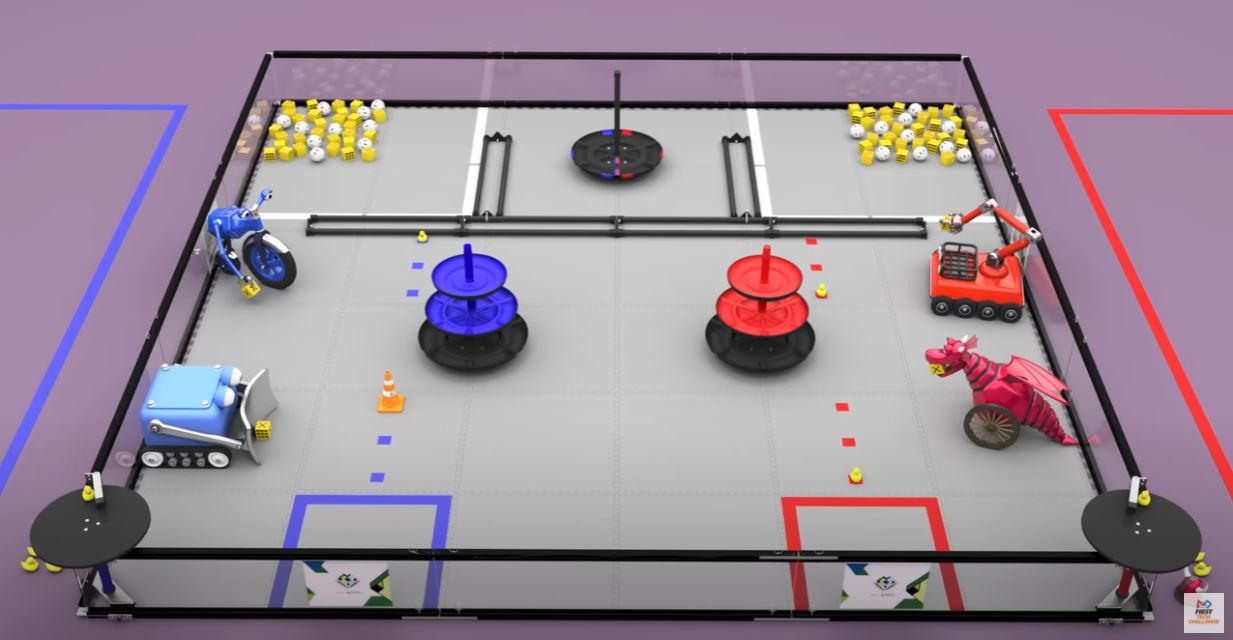
\includegraphics[width=0.95\textwidth]{Meetings/September/09-21-21/9-18-21_Team_Image2 - Nathan Forrer.jpg}
  \caption{This year's field.}
  \label{fig:pic2}
\end{minipage}
\end{figure}

\begin{figure}[ht]
\centering
\begin{minipage}[b]{.48\textwidth}
  \centering
  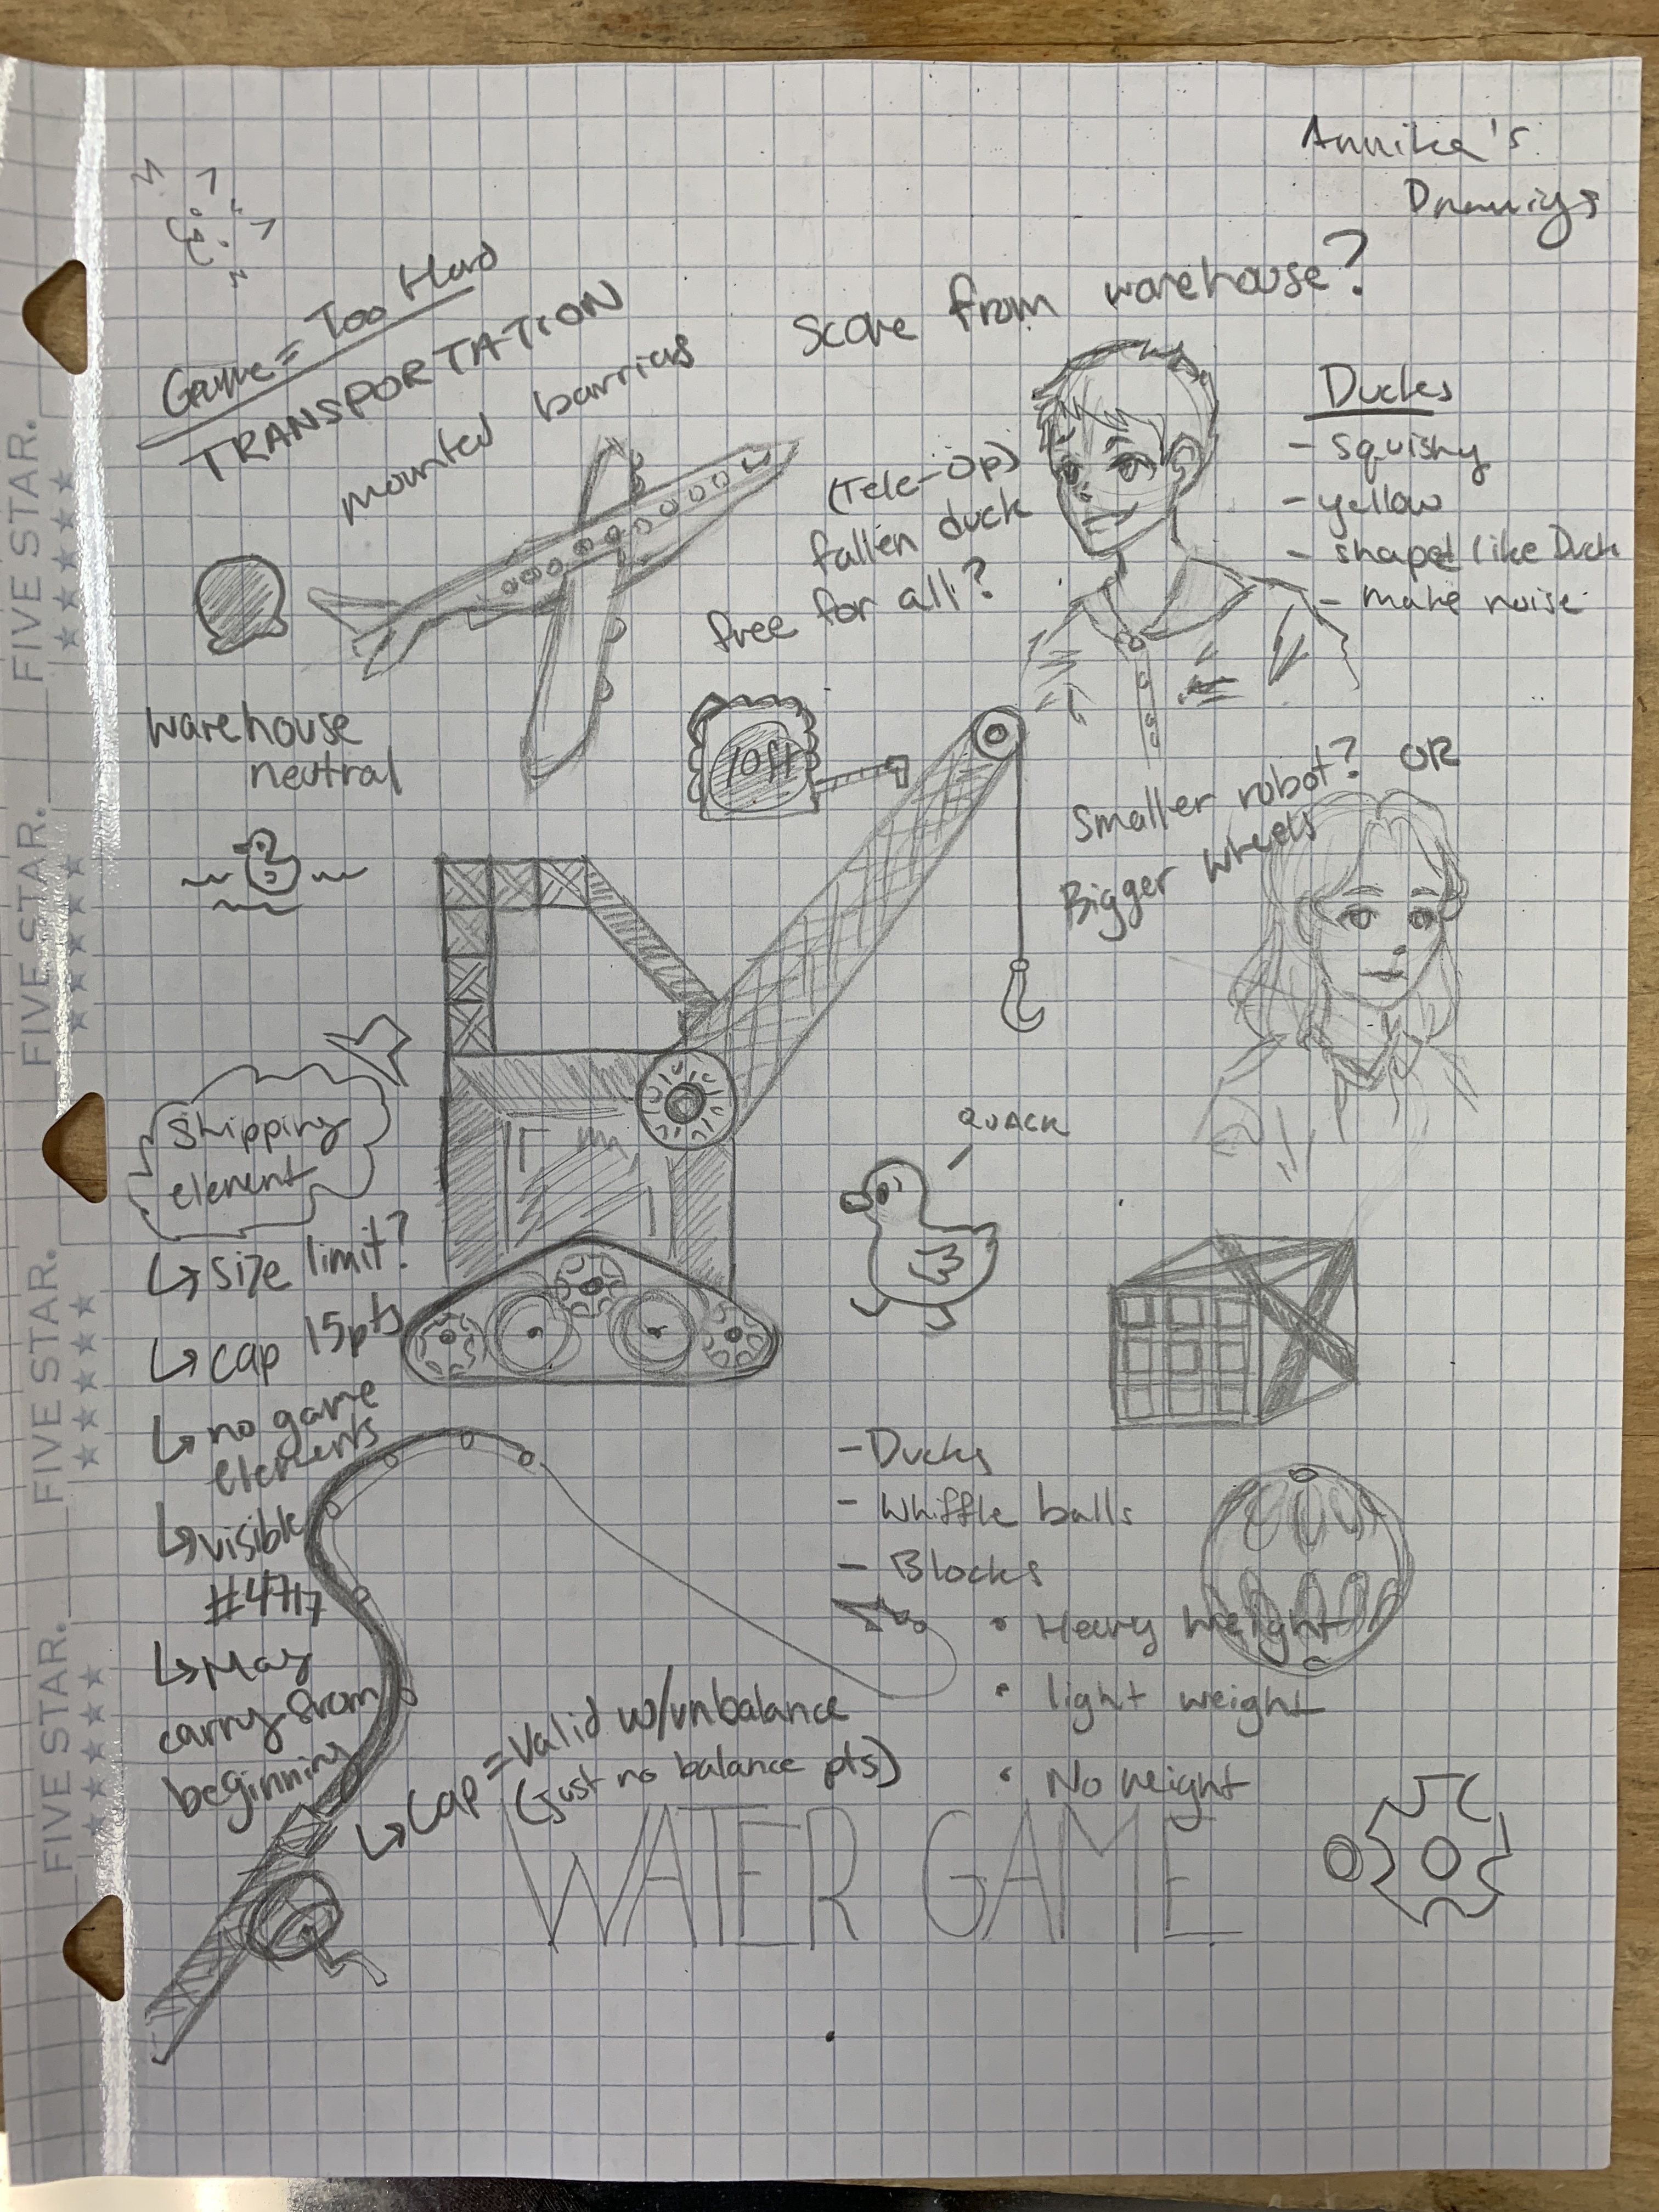
\includegraphics[width=0.95\textwidth]{Meetings/September/09-21-21/9-19-21_Team_Image3 - Nathan Forrer.JPG}
  \caption{A robot doodle page (With some bonus drawings).}
  \label{fig:pic3}
\end{minipage}%
\hfill%
\begin{minipage}[b]{.48\textwidth}
  \centering
  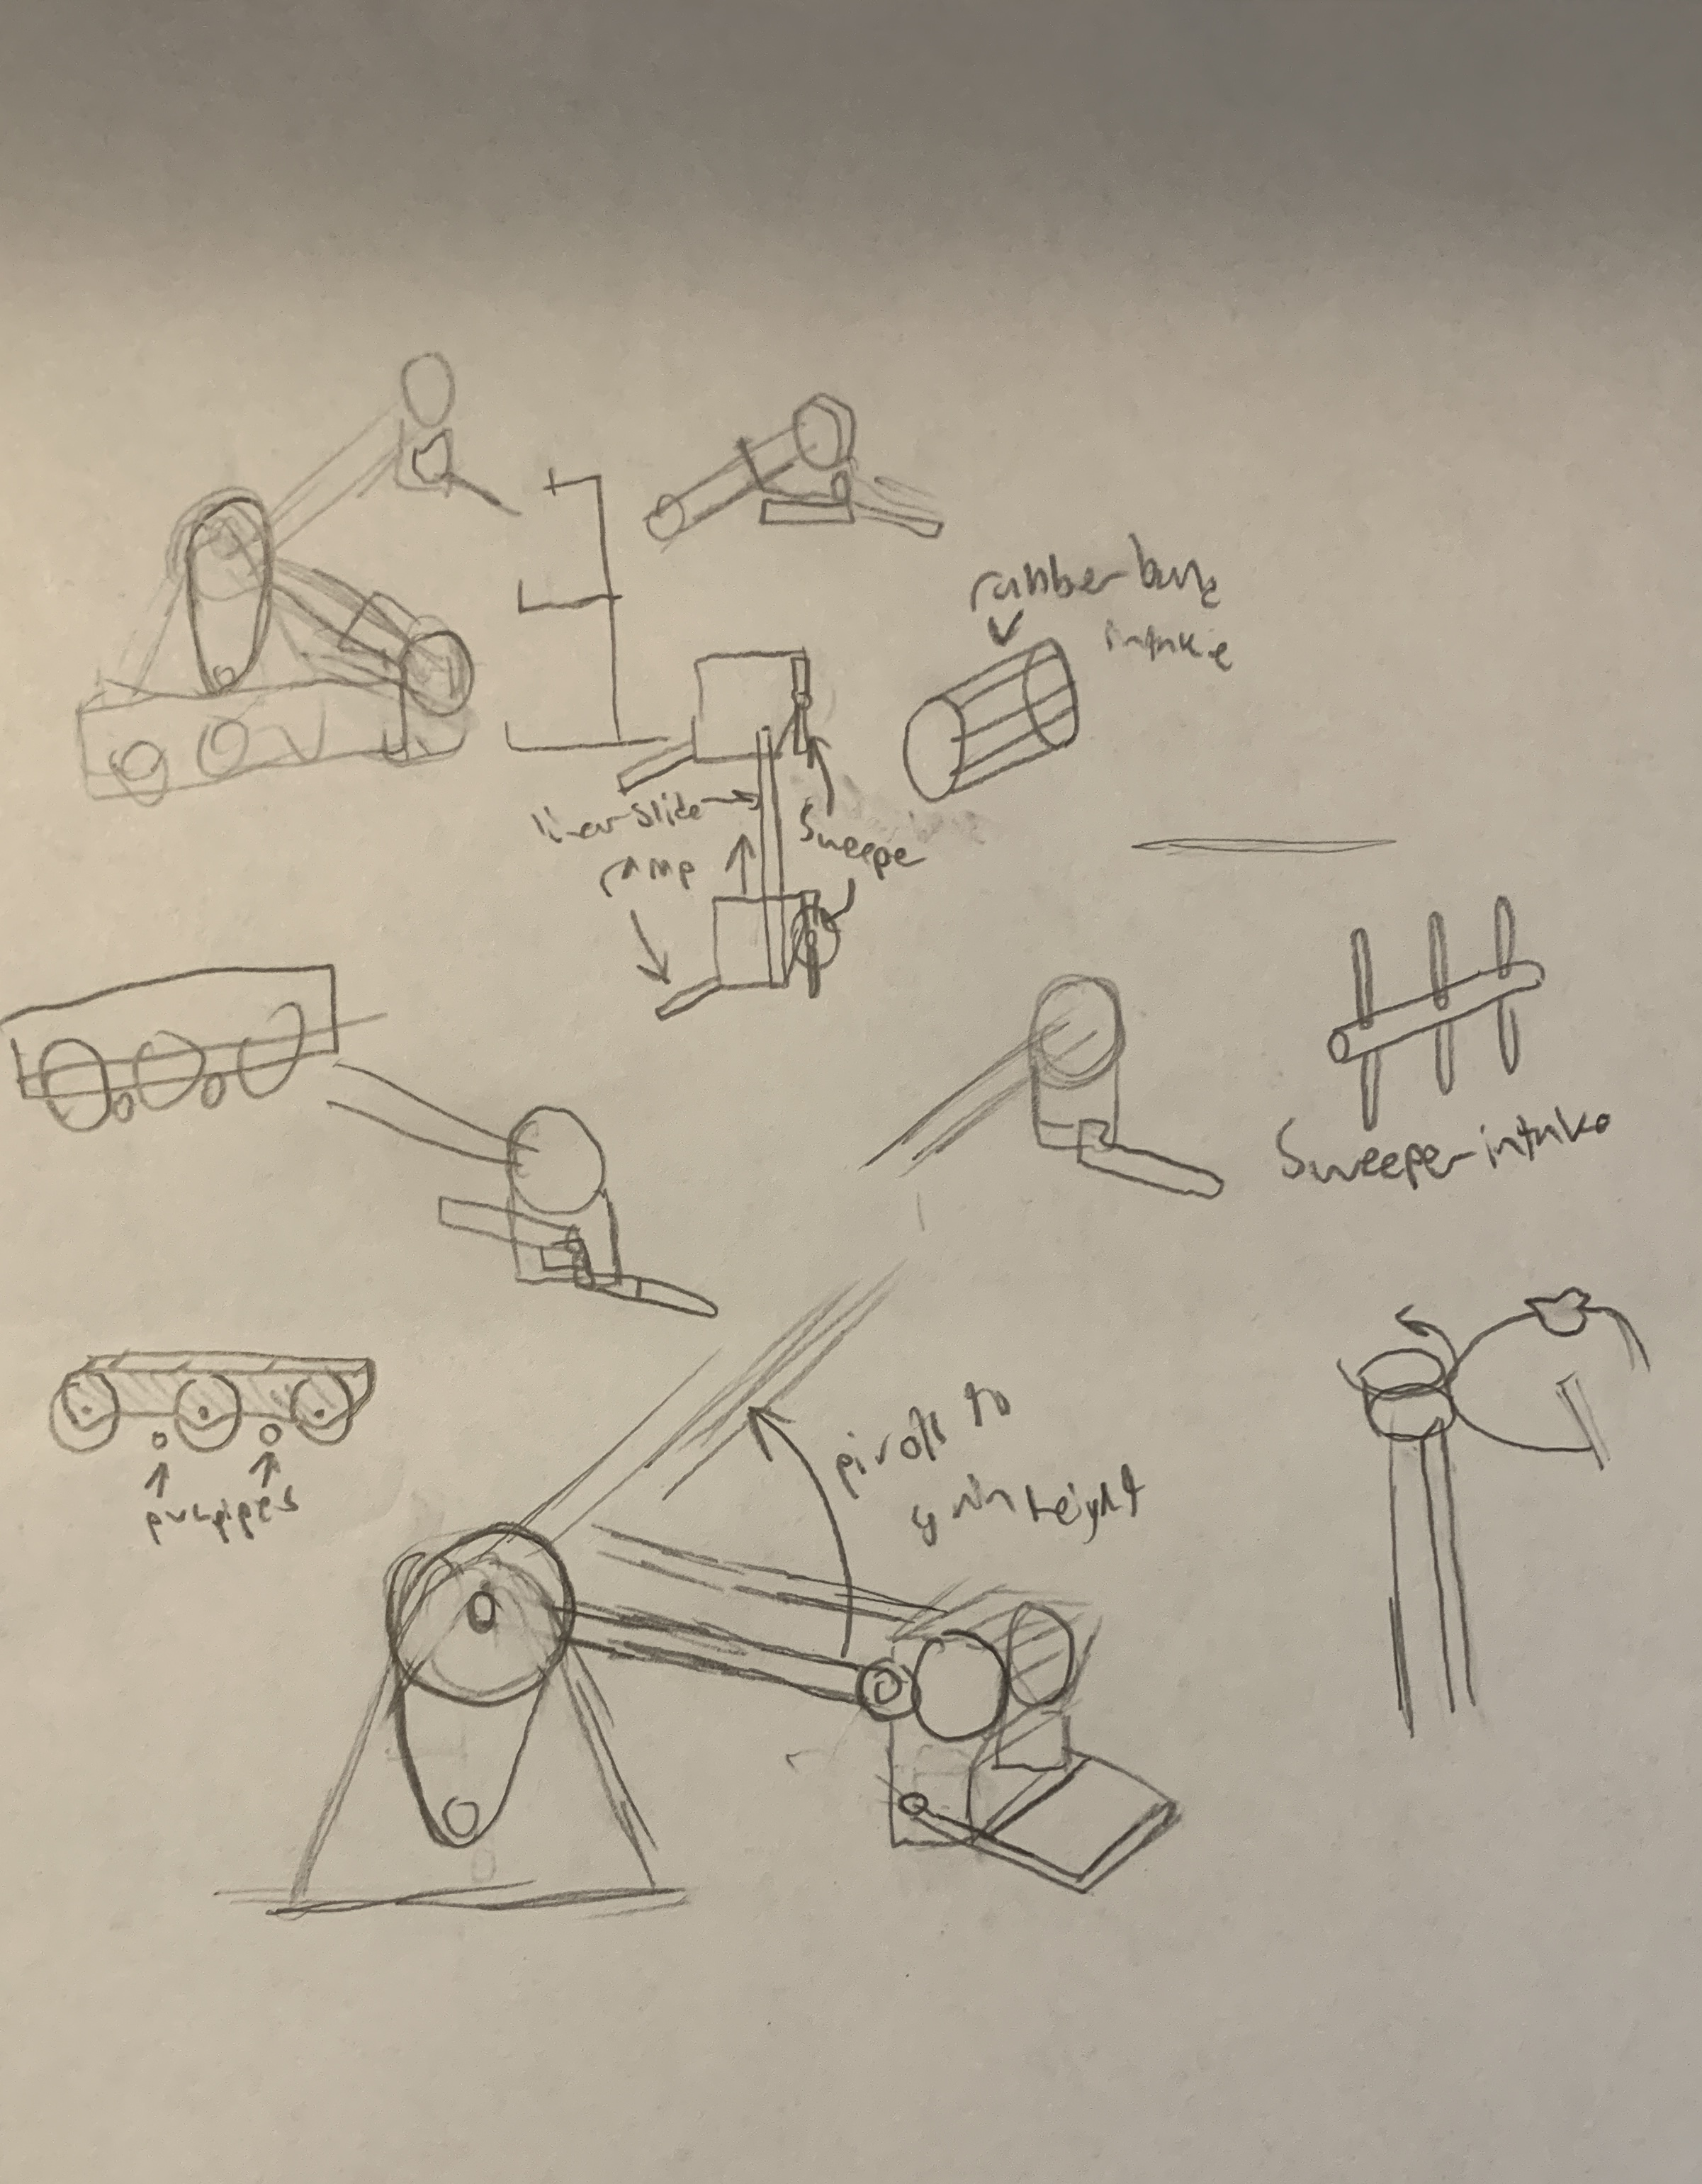
\includegraphics[width=0.95\textwidth]{Meetings/September/09-21-21/9-19-21_Team_Image4 - Nathan Forrer.JPG}
  \caption{Another page of our team's planning sketches.}
  \label{fig:pic4}
\end{minipage}
\end{figure}

\begin{figure}[ht]
\centering
\begin{minipage}[b]{.48\textwidth}
  \centering
  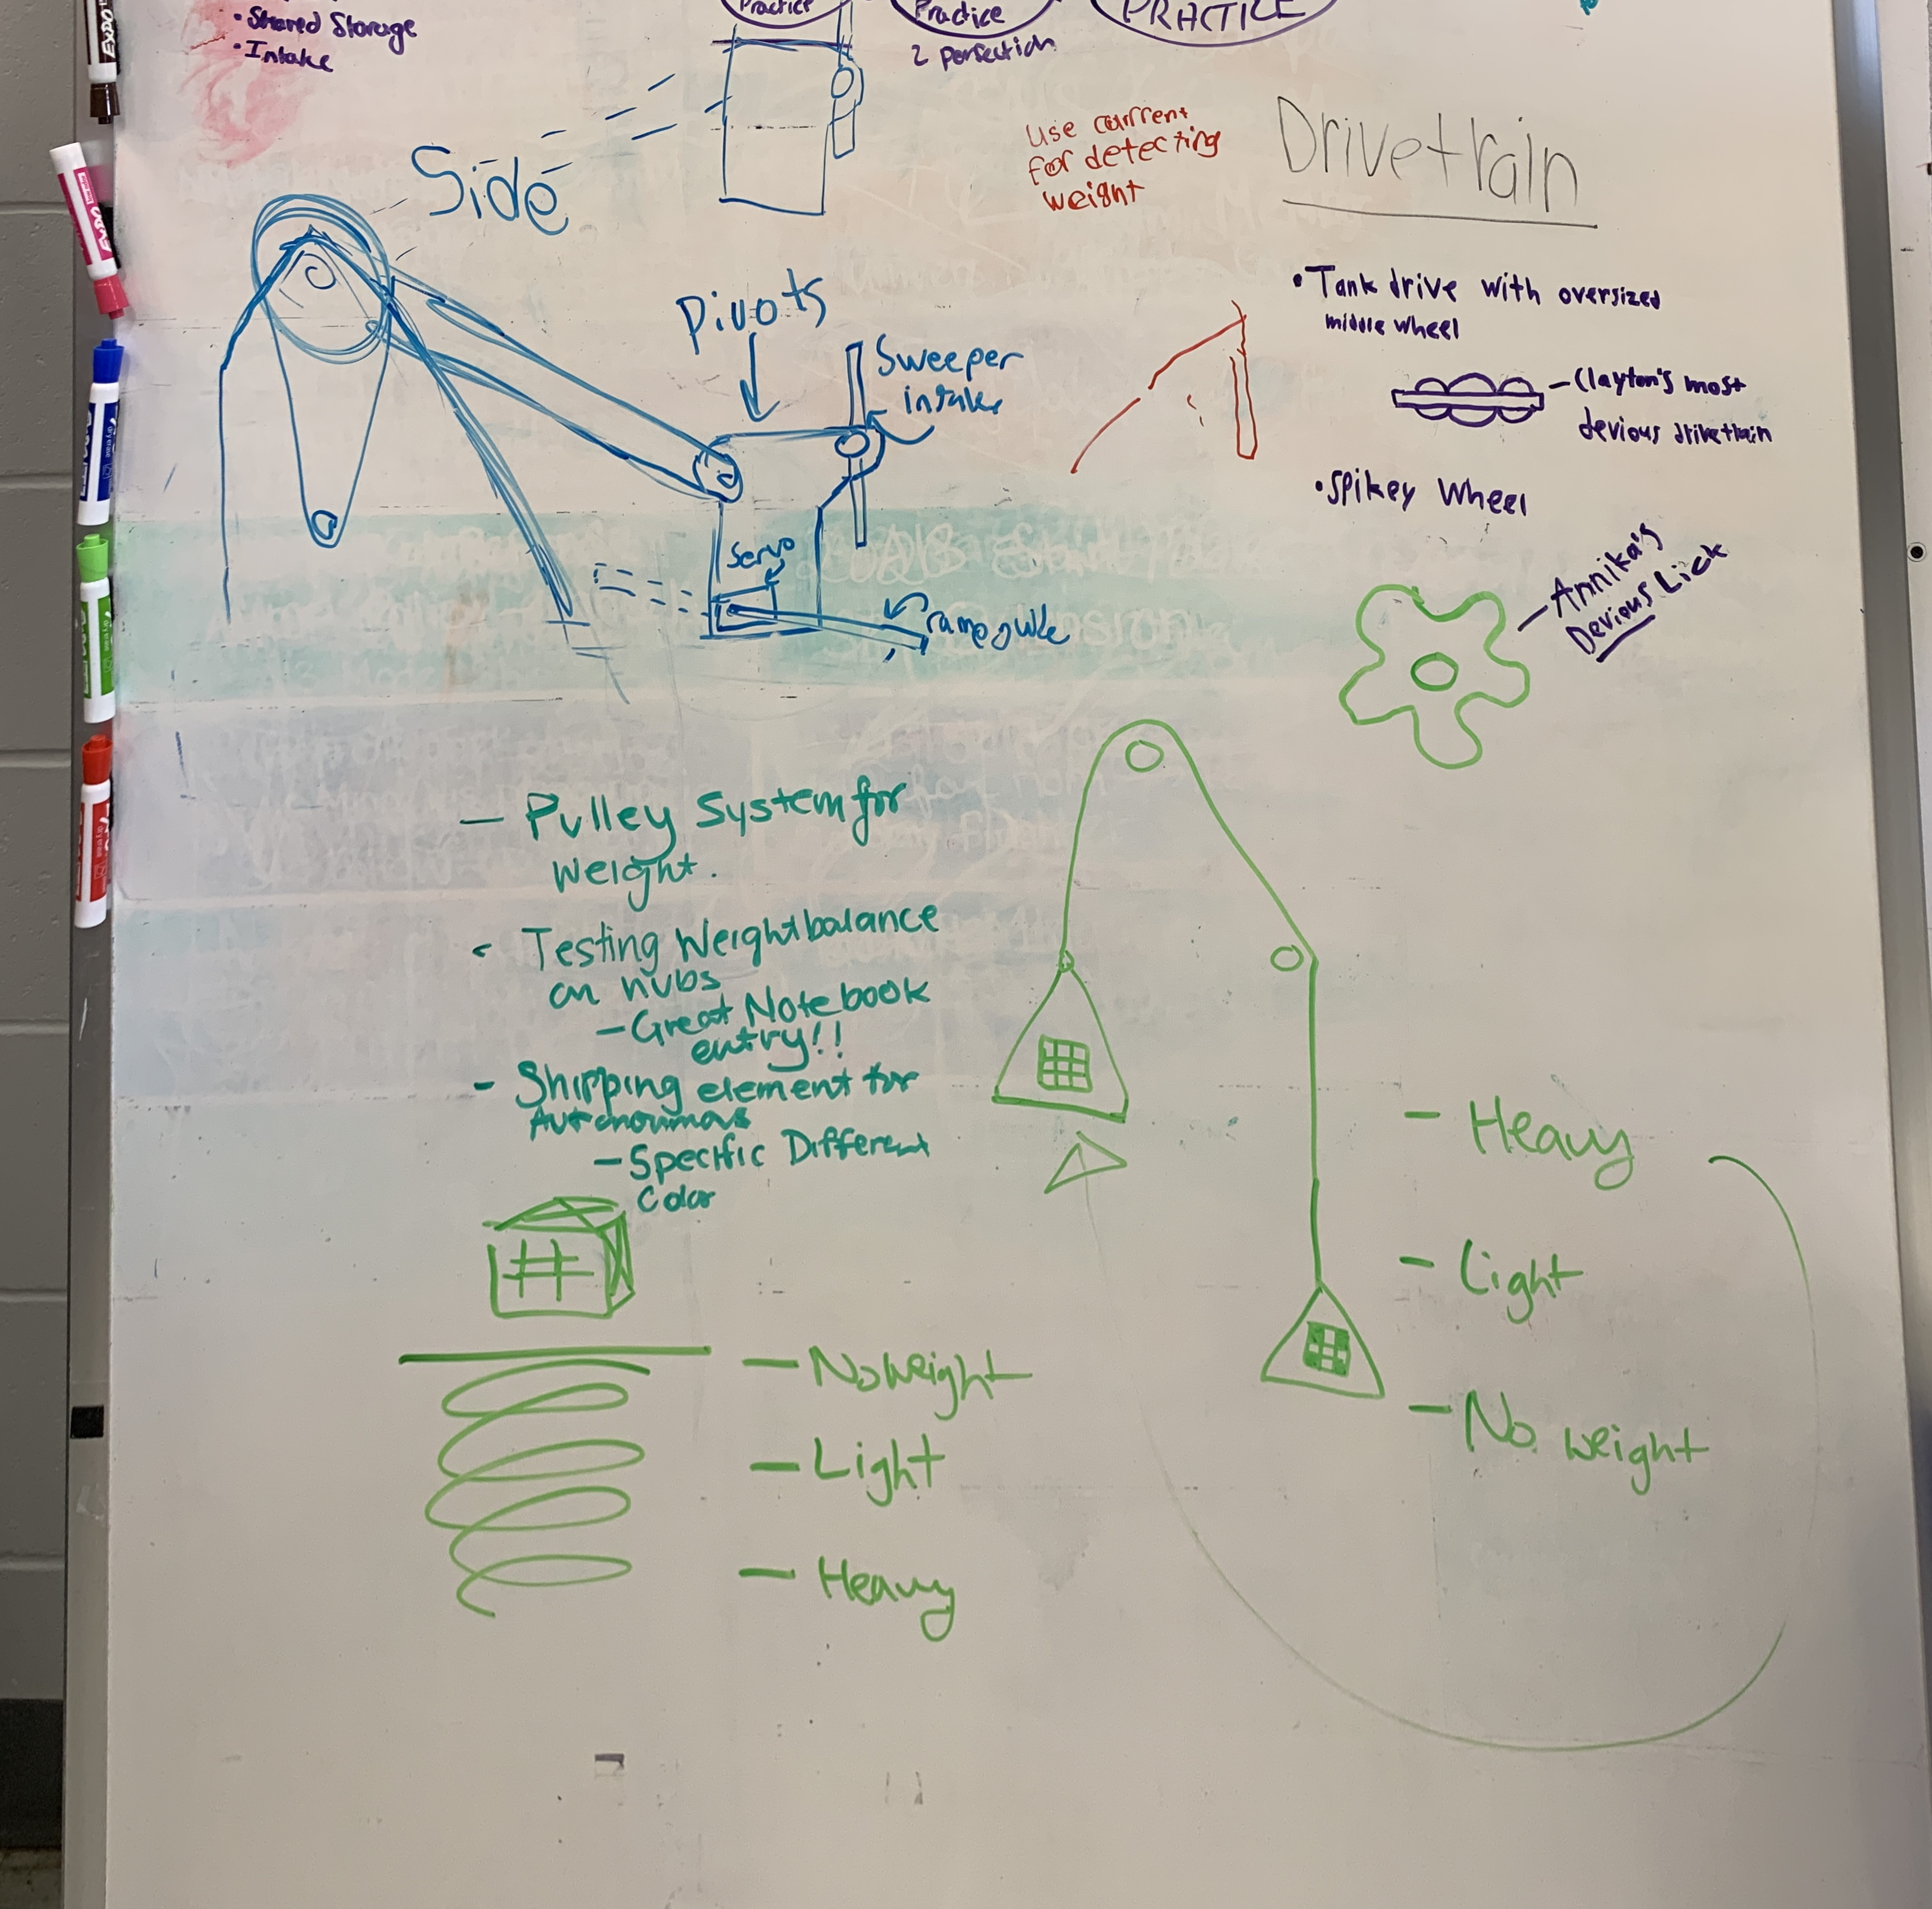
\includegraphics[width=0.95\textwidth]{Meetings/September/09-21-21/9-19-21_Team_Image5 - Nathan Forrer.JPG}
  \caption{A whiteboard with even more of our team's planning.}
  \label{fig:pic5}
\end{minipage}%
\hfill%
\begin{minipage}[b]{.48\textwidth}
  \centering
  \includegraphics[width=0.95\textwidth]{Meetings/September/09-21-21/9-19-21_Team_Image6 - Nathan Forrer.JPG}
  \caption{Jensen and Annika prototyping designs.}
  \label{fig:pic6}
\end{minipage}
\end{figure}

\begin{figure}[ht]
\centering
\begin{minipage}[b]{.48\textwidth}
  \centering
  \includegraphics[width=0.95\textwidth]{Meetings/September/09-21-21/9-18-21_Team_Image7 - Nathan Forrer.jpg}
  \caption{A closeup shot of our brainstorms on a pulley system.}
  \label{fig:pic7}
\end{minipage}%
\hfill%
\begin{minipage}[b]{.48\textwidth}
  \centering
  \includegraphics[width=0.95\textwidth]{Meetings/September/09-21-21/9-18-21_Team_Image8 - Nathan Forrer.jpg}
  \caption{Our timeline for this year.}
  \label{fig:pic8}
\end{minipage}
\end{figure}



%%%%%%%%%%%%%%%%%%%%%%%%%%%%%%%%%%%%%%%%%%%%%%
%                insertmeeting
% 1) Title (something creative & funny?)
% 2) Date (MM/DD/YYYY)
% 3) Location (ex. Hagerty High School)
% 4) People/Committees Present 
% 5) Picture 
% 6) Start Time & Stop Time (ex. 12:30AM to 4:30PM)
%%%%%%%%%%%%%%%%%%%%%%%%%%%%%%%%%%%%%%%%%%%%%%
\insertmeeting 
	{Let's Get Digital} 
	{09/23/21}
	{Hagerty High School}
	{Austin English, Ryan Nelson}
	{Images/RobotPics/robot.jpg}
	{2:30 - 4:30}
	
\subsection*{Programming}
\noindent\hfil\rule{\textwidth}{.4pt}\hfil
\subsubsection*{Goals}
\begin{itemize}
    \item Set up Android studio
    \item set up TRC code   
    \item Set up a new Github repository for this years code
    \item Help all new programming team members obtain a github account 
\end{itemize} 

\noindent\hfil\rule{\textwidth}{.4pt}\hfil

\subsubsection*{Accomplishments}
Today, we worked on setting up a 4717 github repository so we can wirelessly communicate between different computers relatively seamlessly. The repository has different folders for CAD and Programming, among others. Each subset has different permissions as to who can access it to prevent accidental changes to our CAD or program. First, we had all the new members create new accounts in GitHub, as shown in Figure \ref{fig:pic1}. Everyone contributes to the repository, as shown in Figure \ref{fig:pic2}. In order to communicate these files from one person to another, knowing how to pull and push files will be necessary, as shown in Figures \ref{fig:pic3} and \ref{fig:pic4}. 
 
We accomplished our goals of setting up Android studio and the TRC code.
 

\begin{figure}[ht]
\centering
\begin{minipage}[b]{.50\textwidth}
  \centering
  \includegraphics[width=0.5\textwidth]{Meetings/September/09-23-21/githubnewacc.png}
  \caption{New Account in Github}
  \label{fig:pic1}
\end{minipage}%
\hfill%
\begin{minipage}[b]{.50\textwidth}
  \centering
  \includegraphics[width=0.8\textwidth]{Meetings/September/09-23-21/githubrepository.png}
  \caption{Screenshot of GitHub Repository}
  \label{fig:pic2}
\end{minipage}
\end{figure}




\begin{figure}
\centering
\includegraphics[width=0.85\textwidth, angle=0]{Meetings/September/09-23-21/gitshellpull.png}
\caption{GitShell Pull Files}
\label{fig:pic3}
\end{figure}


\begin{figure}
\centering
\includegraphics[width=0.85\textwidth, angle=0]{Meetings/September/09-23-21/gitshellpush.png}
\caption{GitShell Push Files}
\label{fig:pic4}
\end{figure}








%%%%%%%%%%%%%%%%%%%%%%%%%%%%%%%%%%%%%%%%%%%%%%
%                insertmeeting
% 1) Title (something creative & funny?)
% 2) Date (MM/DD/YYYY)
% 3) Location (ex. Hagerty High School)
% 4) People/Committees Present 
% 5) Picture 
% 6) Start Time & Stop Time (ex. 12:30AM to 4:30PM)
%%%%%%%%%%%%%%%%%%%%%%%%%%%%%%%%%%%%%%%%%%%%%%
\insertmeeting 
	{Merry-Go-Round} 
	{09/28/21}
	{Hagerty High School}
	{Clayton, Jensen, Nathan, Ritam}
	{Images/RobotPics/robot.jpg}
	{2:30 - 4:30}
	
\hhscommittee{Hardware}
\noindent\hfil\rule{\textwidth}{.4pt}\hfil
\subsubsection*{Goals}
\begin{itemize}
    \item Continue discussing drivetrain
    \item Prototype carousel mechanism
  

\end{itemize} 

\noindent\hfil\rule{\textwidth}{.4pt}\hfil

\subsubsection*{Accomplishments}
Today we started off the meeting by testing out our idea for the carousel. During the reveal, the carousel stuck out as a very simple and easy to complete task to almost every member, making it a prime subject for our first mechanism. We made it our goal to make a prototype for the carousel to see if our idea will work. Our idea is to attach a wheel to a motor that we can put up against the carousell , spinning the ducks off the platform. Building the prototype proved as simple as we had expected, and we soon had attached a REV grip wheel to a REV core hex motor, hooking it all up to a REV hub so we could control it. When we held the motor up to the carousel, it spun just as we had expected (image 1). Because of the speed of the core hex motor, the duck didn’t fall off of the carousel even at maximum speed. This made us question how much faster we could go. To test out this question, we swapped the core hex motor for a HD hex motor with a 20:1 planetary gearbox. Attaching the wheel in the exact same way, we once again held the mechanism up to the carousel. This time, at the motor’s max speed, the duck flew off (image 2). This means that if we use the faster HD hex motor and slow the speed down slightly in software, we will be able to move at the fastest speed without the duck falling off using the controller, we were able to get the speed pretty fast without making the duck fall off (image 3). 
Another strategy we have for ensuring the duck doesn’t fall off of the carousel takes advantage of the mathematical properties of linear and angular velocity. When we put the duck closer to the center of the carousel, its linear velocity, or how far the duck is actually moving, is lower, meaning the centrifugal force on the duck is lower. When this force is lower, there is less of a chance of the duck flying off the carousel. Usually, if you decrease the velocity, it will take longer for something to go the same distance, but because the carousel is rotating, putting the duck closer to the center does not change the angular velocity, or how many rotations the duck is moving in a certain amount of time. By moving the duck closer to the center, we decrease the linear velocity and the forces applied to the duck, but the angular velocity remains unchanged, meaning it won’t cost us any time. A mathematical proof is shown below: (image 4)

Moving on to the drivetrain, over the weekend, several teams uploaded robot in 3 days (Ri3D) robot reveals. By watching the simple prototyping of some other teams, we saw that formal drivetrains like mecanum and tank can still go over the barrier poles, as long as the wheels hit the poles first. This might mean that a completely new drivetrain design won’t be necessary and we can use a similar basic design that we’ve been adjusting and changing to fit new needs every year. We still plan on creating the lighter, 4 wheeled tank drive prototype once the parts arrive, but to keep our options open, we are also going to test our designs from previous years as well.
The first design that we are going to test is the mecanum drivetrain that we designed and built over the summer. We are happy to know that this drivetrain might still have a use for us during this season, but because we didn’t think it would go over the barriers, we left it in a partial state of disrepair. When the game reveal came out, we were in the middle of adding spacers to the wheels and replacing all of the shafts, but we never finished doing all of this. Because we have a newfound use for the drivetrain, we still need to rebuild it. Using a small chop saw in our room, we cut a steel shaft into the correct length for our wheels (image 5). Once the shafts were cut, we pressed them into the pulleys, added the spacers into the wheels and put the rest of the drivetrain back together. At this point in the meeting, we ran out of time, but we still plan on testing the mecanum drive, and our 6- wheel tank drive.


\begin{figure}[ht]
\centering
\begin{minipage}[b]{.48\textwidth}
  \centering
  \includegraphics[width=0.95\textwidth]{Meetings/September/09-28-21/9-28-21_Hardware_Image1 - Nathan Forrer.jpg}
  \caption{Using a traction wheel to prototype a carousel spinner.}
  \label{fig:pic1}
\end{minipage}%
\hfill%
\begin{minipage}[b]{.48\textwidth}
  \centering
  \includegraphics[width=0.95\textwidth]{Meetings/September/09-28-21/9-28-21_Hardware_Image2 - Nathan Forrer.jpg}
  \caption{Another angle of our prototype.}
  \label{fig:pic2}
\end{minipage}
\end{figure}

\begin{figure}[ht]
\centering
\begin{minipage}[b]{.48\textwidth}
  \centering
  \includegraphics[width=0.95\textwidth]{Meetings/September/09-28-21/9-28-21_Hardware_Image3 - Nathan Forrer.jpg}
  \caption{The prototype in action.}
  \label{fig:pic3}
\end{minipage}%
\hfill%
\begin{minipage}[b]{.48\textwidth}
  \centering
  \includegraphics[width=0.95\textwidth]{Meetings/September/09-28-21/9-28-21_Hardware_Image4 - Nathan Forrer.jpg}
  \caption{The calculations used in designing a carousel spinner mechanism.}
  \label{fig:pic4}
\end{minipage}
\end{figure}

\begin{figure}[htp]
\centering
  \includegraphics[width=0.95\textwidth]{Meetings/September/09-28-21/9-28-21_Hardware_Image5 - Nathan Forrer.jpg}
  \caption{Nathan cutting a hex shaft using a chopsaw.}
  \label{fig:pic5}
\end{figure}


\whatsnext{
\begin{itemize}
    \item Test mecanum drive
    \item Fix and test 6- wheel tank drive
    \item Build prototype 4 wheel tank drive.

\end{itemize} 
}


%%%%%%%%%%%%%%%%%%%%%%%%%%%%%%%%%%%%%%%%%%%%%%
%                insertmeeting
% 1) Title (something creative & funny?)
% 2) Date (MM/DD/YYYY)
% 3) Location (ex. Hagerty High School)
% 4) People/Committees Present 
% 5) Picture 
% 6) Start Time & Stop Time (ex. 12:30AM to 4:30PM)
%%%%%%%%%%%%%%%%%%%%%%%%%%%%%%%%%%%%%%%%%%%%%%
\insertmeeting 
	{Mecanum Madness Part 2} 
	{09/30/21}
	{Hagerty High School}
	{Clayton, Jensen, Nathan, Ritam}
	{Images/RobotPics/robot.jpg}
	{2:30 - 4:30}
	
\hhscommittee{Hardware}
\noindent\hfil\rule{\textwidth}{.4pt}\hfil
\subsubsection*{Goals}
\begin{itemize}
    \item Set up field
    \item Test mecanum drive
 

\end{itemize} 

\noindent\hfil\rule{\textwidth}{.4pt}\hfil

\subsubsection*{Accomplishments}
After getting the mecanum drivetrain rebuilt last meeting, we are almost ready to test. Before we can, however, we need to set up the field. Because our school also has two vex teams, we have to share the field, so we started setting up half of the field for Freight Frenzy. Although we have already set up the carousel, we still needed to add all of the tape and the barriers (image 1). While setting up the barriers, we realized that if they weren’t ziptied really tight, they shifted slightly. This might make it harder for the robot to go over  them during a competition if they aren’t set up really well. Noticing this, we noted that we will need to ensure our robot can still get over the barriers even if they are a bit loose. Once the barriers were up, we reorganized the wires on the drivetrain to prevent them from getting caught in the wheels or interfering with our testing in any way (image 2). 
Finally, it was time to test the mecanum drive. Just as we had hoped, the mecanum drivetrain flew over the  barriers with little issue. Because of the shape of the drivetrain (image 4), the wheels hit the pipes before the drive plates do, making it easily pull itself over the barrier. On the back of the drivetrain, we didn’t design a cutout for the wheels, making the plates and the wheels hit the  pipes at about the same time. We noticed that although the robot could still drive over the barriers backwards, it isn’t nearly as smooth. This clearly necessitates the need for a wheel cutout on both sides. Seeing how the mecanum drive performed, we are optimistic about the tank drive, which will have more traction than the mecanum drive does. With the addition of the middle drop center wheel, the possibility of getting stuck should be reduced. That being said, the tank drive design that we currently have to test has much lower plates and motors, so in its current state, it may not go over the barrier as smoothly. We were already planning on making some design changes, but we still hope to test the current design soon.

 

\begin{figure}[ht]
\centering
\begin{minipage}[b]{.48\textwidth}
  \centering
  \includegraphics[width=0.95\textwidth]{Meetings/September/09-30-21/9-30-21_Hardware_Image1 - Nathan Forrer.jpg}
  \caption{Anouska and Samantha setting up the field with tape.}
  \label{fig:pic1}
\end{minipage}%
\hfill%
\begin{minipage}[b]{.48\textwidth}
  \centering
  \includegraphics[width=0.95\textwidth]{Meetings/September/09-30-21/9-30-21_Hardware_Image2 - Nathan Forrer.jpg}
  \caption{Jensen wiring the Mecanum drive.}
  \label{fig:pic2}
\end{minipage}
\end{figure}

\begin{figure}[ht]
\centering
\begin{minipage}[b]{.48\textwidth}
  \centering
  \includegraphics[width=0.95\textwidth]{Meetings/September/09-30-21/9-30-21_Hardware_Image3 - Nathan Forrer.JPG}
  \caption{Testing the mecanum drive's ability to move over the barrier.}
  \label{fig:pic1}
\end{minipage}%
\hfill%
\begin{minipage}[b]{.48\textwidth}
  \centering
  \includegraphics[width=0.95\textwidth]{Meetings/September/09-30-21/9-30-21_Hardware_Image4 - Nathan Forrer.JPG}
  \caption{Our CAD drawing for the driveplates.}
  \label{fig:pic2}
\end{minipage}
\end{figure}

\whatsnext{
\begin{itemize}
    \item Test tank drive
    \item Build prototype 4 wheel tank drive

\end{itemize} 
}
% 1) Title
% 2) Date
% 3) Location
% 4) Present
% 5) Picture
% 6) Start Time
% 7) Stop Time
\insertmeeting 
	{Meeting Example} 
	{09/18/21}
	{Hagerty High School}
	{Jenson}
	{Images/RobotPics/robot.jpg}
	{2:30}
  {4:30}
	
\section*{General}
\noindent\hfil\rule{\textwidth}{.4pt}\hfil
\subsection*{Goals}
\begin{itemize}
    \item Watch kickoff
    \item Brainstorm   

\end{itemize} 

\noindent\hfil\rule{\textwidth}{.4pt}\hfil

\subsection*{Accomplishments}
Today, we watched the kickoff.
 

\begin{figure}[ht]
\centering
\begin{minipage}[b]{.50\textwidth}
  \centering
  \includegraphics[width=0.8\textwidth]{Meetings/September/09-18-21/field.png}
  \caption{New Account in Github}
  \label{fig:pic1}
\end{minipage}%
\hfill%
\begin{minipage}[b]{.50\textwidth}
  \centering
  \includegraphics[width=0.8\textwidth]{Meetings/September/09-18-21/field.png}
  \caption{Screenshot of GitHub Repository}
  \label{fig:pic2}
\end{minipage}
\end{figure}








%%%%%%%%%%%%%%%%%%%%%%%%%%%%%%%%%%%%%%%%%%%%%%
%                insertmeeting
% 1) Title (something creative & funny?)
% 2) Date (MM/DD/YYYY)
% 3) Location (ex. Hagerty High School)
% 4) People/Committees Present 
% 5) Picture 
% 6) Start Time & Stop Time (ex. 12:30AM to 4:30PM)
%%%%%%%%%%%%%%%%%%%%%%%%%%%%%%%%%%%%%%%%%%%%%%
\insertmeeting 
	{Imperfect Prototyping} 
	{10/07/21}
	{Hagerty High School}
	{Annika, Anouska, Jensen, Nathan, Ritam, Rose, Samantha}
	{Images/RobotPics/robot.jpg}
	{2:30 - 4:30}
	
\subsection*{Hardware}
\noindent\hfil\rule{\textwidth}{.4pt}\hfil
\subsubsection*{Goals}
\begin{itemize}
    \item set up rev hub
    \item build simple arm 

\end{itemize} 

\noindent\hfil\rule{\textwidth}{.4pt}\hfil

\subsubsection*{Accomplishments}
Now that we have the prototype drivetrain built, we decided to continue working and prototyping with it. Because it is constructed out of rev parts, prototyping was far more effiecent than seen with our other designs. Although we have a couple more drivetrain designs we want to build and test, this small 4 wheel tank drive will be fit for most of our basic prototyping. Before we started doing anything else, we needed to get all of the many different electronic components hooked up to the drivetrain. To accomplish this we CADed a middle plate with mounting holes for the Rev hub and battery (Figure \ref{fig:pic1}). From there, we connected the components, downloaded the code and did a test drive.Fortunatley we found that the drivetrain worked very well! The speed was very apparent from the start with this design, which meant that turning was pretty in precise. We started brainstorming about how to make smaller adjustments possible while still preserving the speed. Although we could come up with a software solution, we would have to slow down all of the movement, which will decrease efficiency. One idea we all found enticing was making a car drive. The way a car works is the back wheels are powered and the front wheel pivots, controlling the steering. This would allow us to make fine adjustments while keeping its breakneck speed. Another thing we like about this design is that it is very unique. We are not aware of any team making a drivetrain like this in ftc, so it would differentiate us from all of the other teams this year. To get a better idea of what the drivetrain would look like, we made some sketches we could hand over to the cad committee (Figure \ref{fig:pic2}).
While the cad committee worked on the car drive, we started constructing the arm. The arm connects to the drivetrain with a frame we built out of rev extrusions (Figure \ref{fig:pic3}). After constructing this frame we attached a motor and some bearing brackets. We then used a gear to attach the arm, which is just a long rev extrusion, to the motor. At the end of the arm, we started constructing the first half off our claw. Resembling a spatula (Figure \ref{fig:pic4}), this part of the claw will slide under a block and another part of the claw, which we will construct at a future meeting, will pivot down and clamp a block or ball into the robot.
 

\begin{figure}[ht]
\centering
\begin{minipage}[b]{.50\textwidth}
  \centering
  \includegraphics[width=0.8\textwidth]{Meetings/October/10-07-21/10-7-21_Hardware_Figure1 - Nathan Forrer.PNG}
  \caption{Our current RevHub mount with the new holes.}
  \label{fig:pic1}
\end{minipage}%
\hfill%
\begin{minipage}[b]{.50\textwidth}
  \centering
  \includegraphics[width=0.8\textwidth]{Meetings/October/10-07-21/10-7-21_Hardware_Figure2 - Nathan Forrer.JPG}
  \caption{Initial sketches of the tricycle drivebase.}
  \label{fig:pic2}
\end{minipage}
\end{figure}

\begin{figure}[ht]
\centering
\begin{minipage}[b]{.50\textwidth}
  \centering
  \includegraphics[width=0.8\textwidth]{Meetings/October/10-07-21/10-7-21_Hardware_Figure3 - Nathan Forrer.JPG}
  \caption{Our arm pivot mechanism.}
  \label{fig:pic3}
\end{minipage}%
\hfill%
\begin{minipage}[b]{.50\textwidth}
  \centering
  \includegraphics[width=0.8\textwidth]{Meetings/October/10-07-21/10-7-21_Hardware_Figure4 - Nathan Forrer.JPG}
  \caption{The first piece of our intake.}
  \label{fig:pic4}
\end{minipage}
\end{figure}
%%%%%%%%%%%%%%%%%%%%%%%%%%%%%%%%%%%%%%%%%%%%%%
%                insertmeeting
% 1) Title (something creative & funny?)
% 2) Date (MM/DD/YYYY)
% 3) Location (ex. Hagerty High School)
% 4) People/Committees Present 
% 5) Picture 
% 6) Start Time & Stop Time (ex. 12:30AM to 4:30PM)
%%%%%%%%%%%%%%%%%%%%%%%%%%%%%%%%%%%%%%%%%%%%%%
\insertmeeting 
	{First Field Test} 
	{10/12/21}
	{Hagerty High School}
	{Annika, Anouska, Clayton, Falon, James, Jensen, Nathan, Ritam, Rose, Samantha, Lilly}
	{Images/RobotPics/robot.jpg}
	{2:30 - 4:30}
	
\subsection*{General}
\noindent\hfil\rule{\textwidth}{.4pt}\hfil
\subsubsection*{Goals}
\begin{itemize}
    \item Practice driving tank robot
    \item Evaluate and fix issues 

\end{itemize} 

\noindent\hfil\rule{\textwidth}{.4pt}\hfil

\subsubsection*{Accomplishments}
At this team meeting, we did the first field test of our tank drive robot!  Before we got started however, our software team created a tele-op program. Instead of using standard tank controls, we decided to use arcade drive, where one stick controls tuning and the other controls speed. This will make our driving a bit smoother going around corners. With everything ready, we started driving the robot around the field, doing as many cycles as possible. We quickly found out that driver practice was going to be very important this year, especially because of our lack of experience. What we saw was that most of the time was spent going through the gap in the barriers and turning the corner to head towards the shipping hub (Figure \ref{fig:pic1}). Using the car drive should make this process a bit easier, but we came up with the idea to make some round parts that attach onto the corners that reduce damage from slamming against the wall, so we CADed and cut them, and attached them to the robot (Figure \ref{fig:pic2}). 
One other issue we faced was the robot dropping the block as we lifted the arm, a problem that slowed us down significantly. We came up with two separate ideas on how to fix this; one software, and one hardware. For the software solution we wanted to slow down the movement of the arm as it rotates upwards so that less force is exerted on the block. To do this, we came up with an equation for the position and speed of the arm and graphed it on a graphing calculator to ensure it was correct (Figure \ref{fig:pic3}. The hardware solution involved changing the grabber to hold the block more firmly. One way to do this is to move the servo mount forward so that the center of rotation is closer to the cargo we are trying to pick up. Moving the servo forward will also make the grabber shorter, so it won't get caught on the shipping hub, as we saw a few times during our testing.  Another way we planned to improve the hardware was to expand the width of the grabber, creating more friction on the block we are picking up, ensuring it doesn’t fall out before we open the grabber. We made all these changes in CAD, cut out all the parts on the glowforge, then attached it to the robot (Figure \ref{fig:pic4}). With all of these changes, we plan on testing them out in a future meeting.
 

\begin{figure}[ht]
\centering
\begin{minipage}[b]{.50\textwidth}
  \centering
  \includegraphics[width=0.8\textwidth]{Meetings/October/10-12-21/10-12-21_Team_Figure1 - Nathan Forrer.JPG}
  \caption{Clayton and Jensen driving the new robot.}
  \label{fig:pic1}
\end{minipage}%
\hfill%
\begin{minipage}[b]{.50\textwidth}
  \centering
  \includegraphics[width=0.8\textwidth]{Meetings/October/10-12-21/10-12-21_Team_Figure2 - Nathan Forrer.JPG}
  \caption{New rounded parts.}
  \label{fig:pic2}
\end{minipage}
\end{figure}

\begin{figure}[ht]
\centering
\begin{minipage}[b]{.50\textwidth}
  \centering
  \includegraphics[width=0.8\textwidth]{Meetings/October/10-12-21/10-12-21_Team_Figure3 - Nathan Forrer.PNG}
  \caption{Equation for controlling the arm.}
  \label{fig:pic3}
\end{minipage}%
\hfill%
\begin{minipage}[b]{.50\textwidth}
  \centering
  \includegraphics[width=0.8\textwidth]{Meetings/October/10-12-21/10-12-21_Team_Figure4 - Nathan Forrer.JPG}
  \caption{The grabber.}
  \label{fig:pic4}
\end{minipage}
\end{figure}
%%%%%%%%%%%%%%%%%%%%%%%%%%%%%%%%%%%%%%%%%%%%%%
%                insertmeeting
% 1) Title (something creative & funny?)
% 2) Date (MM/DD/YYYY)
% 3) Location (ex. Hagerty High School)
% 4) People/Committees Present 
% 5) Picture 
% 6) Start Time & Stop Time (ex. 12:30AM to 4:30PM)
%%%%%%%%%%%%%%%%%%%%%%%%%%%%%%%%%%%%%%%%%%%%%%
\insertmeeting 
  {Car Drivetrain} 
  {10/14/21}
  {Hagerty High School}
  {Annika, Anouska, Clayton, Falon, Jensen, Nathan, Ritam, Rose, Samantha}
  {Images/RobotPics/robot.jpg}
  {2:30 - 4:30}
  
\hhscommittee{General}
\noindent\hfil\rule{\textwidth}{.4pt}\hfil
\subsubsection*{Goals}
\begin{itemize}
    \item Test drive car drivetrain  

\end{itemize} 

\noindent\hfil\rule{\textwidth}{.4pt}\hfil

\subsubsection*{Accomplishments}
Today we hit a major milestone with our car drivetrain as we drove it around the field for the first time. We had a lot of fun driving it, as it controls very differently to any other robot we’ve ever seen (Figure \ref{fig:pic1}). As the name suggests, it drives more like a car because of its front wheel turning. Despite being very different, controlling the robot started to feel pretty natural as we practiced making cycles. Even without any arm or other mechanism attached, we found that we could drive as fast as the tank drivetrain, and with a little practice, we could be moving extremely quickly. We all were in agreement that this drivetrain has a lot more potential for speed than the tank drive does. With all of this in mind, we decided to continue working with this 3- wheeled car drivetrain, giving hardware the task of designing a 3d printed version.

\begin{figure}[htp]
\centering
\includegraphics[width=0.95\textwidth, angle=0]{Meetings/October/10-14-21/10-14-21_Team_Figure1 - Nathan Forrer.jpg}
\caption{Ritam and Nathan driving the new drivetrain.}
\label{fig:pic1}
\end{figure}

\hhscommittee{Hardware}
\noindent\hfil\rule{\textwidth}{.4pt}\hfil
\subsubsection*{Goals}
\begin{itemize}
    \item Design a 3d printable drivetrain

\end{itemize} 

\noindent\hfil\rule{\textwidth}{.4pt}\hfil

\subsubsection*{Accomplishments}
Today, we started on one of our most daunting tasks yet: designing a 3d printable drivetrain. One of the main challenges of creating this drivetrain is that we have to make it very strong so that it doesn't break when we hit another robot, but we also must keep it light. Seeing the success of the 3 wheeled car drivetrain prototype, we decided that it would be the design we would create. We started making the drivetrain in CAD, designing it around a large rectangular top plate that we can attach electronics and other mechanisms to. Much like with our prototype design, we had to stagger the motors to keep the robot small, but this time we moved the motors towards the front of the robot and plan on connecting them using pulleys (Figure \ref{fig:pic2}). After creating all of the basics, we added strength to the design, using ribs, chamfers and fillets to make the structure more rigid without adding too much weight (Figure \ref{fig:pic3}). Using structures like this allowed us to use 1/8 inch sides for most of the robot, when we normally use 1/4 inch. By being smart about where to add structure, such as around the motors and at other key points, we were able to find what we think is a good balance between strength and weight.

\begin{figure}[ht]
\centering
\begin{minipage}[b]{.48\textwidth}
  \centering
  \includegraphics[width=0.95\textwidth]{Meetings/October/10-14-21/10-14-21_CAD_Figure1.JPG}
  \caption{Current CAD of our drivetrain.}
  \label{fig:pic2}
\end{minipage}%
\hfill%
\begin{minipage}[b]{.48\textwidth}
  \centering
  \includegraphics[width=0.95\textwidth]{Meetings/October/10-14-21/10-14-21_CAD_Figure2.JPG}
  \caption{Our drivetrain's 3D printed base.}
  \label{fig:pic3}
\end{minipage}
\end{figure}

\begin{figure}[htp]
\centering
\includegraphics[width=0.95\textwidth, angle=0]{Meetings/October/10-14-21/10-14-21_Team_Figure1 - Nathan Forrer.jpg}
\caption{Ritam and Nathan driving the new drivetrain.}
\label{fig:pic1}
\end{figure}

\hhscommittee{Hardware}
\noindent\hfil\rule{\textwidth}{.4pt}\hfil
\subsubsection*{Goals}
\begin{itemize}
    \item Design a 3d printable drivetrain

\end{itemize} 

\noindent\hfil\rule{\textwidth}{.4pt}\hfil

\subsubsection*{Accomplishments}
Today, we started on one of our most daunting tasks yet: designing a 3d printable drivetrain. One of the main challenges of creating this drivetrain is that we have to make it very strong so that it doesn't break when we hit another robot, but we also must keep it light. Seeing the success of the 3 wheeled car drivetrain prototype, we decided that it would be the design we would create. We started making the drivetrain in CAD, designing it around a large rectangular top plate that we can attach electronics and other mechanisms to. Much like with our prototype design, we had to stagger the motors to keep the robot small, but this time we moved the motors towards the front of the robot and plan on connecting them using pulleys (Figure \ref{fig:pic2}). After creating all of the basics, we added strength to the design, using ribs, chamfers and fillets to make the structure more rigid without adding too much weight (Figure \ref{fig:pic3}). Using structures like this allowed us to use 1/8 inch sides for most of the robot, when we normally use 1/4 inch. By being smart about where to add structure, such as around the motors and at other key points, we were able to find what we think is a good balance between strength and weight.

\begin{figure}[ht]
\centering
\begin{minipage}[b]{.48\textwidth}
  \centering
  \includegraphics[width=0.95\textwidth]{Meetings/October/10-14-21/10-14-21_CAD_Figure1.JPG}
  \caption{Current CAD of our drivetrain.}
  \label{fig:pic2}
\end{minipage}%
\hfill%
\begin{minipage}[b]{.48\textwidth}
  \centering
  \includegraphics[width=0.95\textwidth]{Meetings/October/10-14-21/10-14-21_CAD_Figure2.JPG}
  \caption{Our drivetrain's 3D printed base.}
  \label{fig:pic3}
\end{minipage}
\end{figure}

\hhscommittee{Outreach}
\noindent\hfil\rule{\textwidth}{.4pt}\hfil
\subsubsection*{Goals}
\begin{itemize}
    \item Installed programming software and prepared for programming for fll
    \item Divided students into 3 teams
 
\end{itemize} 

\noindent\hfil\rule{\textwidth}{.4pt}\hfil

\subsubsection*{Accomplishments}
As our twice a week FLL meetings continue, we are finally moving very close to getting started with the season. At our meeting next Friday, we will finally divide the students up into their competition teams, where they will build their base robots, program their missions, and create their innovation projects. Although we are still a week away from putting them into teams, we started thinking of how we can group them. We decided that the best way for them to get the best out of the program would be to divide them up both by skill and age so that they are all working with teammates with a similar general skill set. To get our thoughts on paper, we created a spreadsheet and put participants in 3 teams tentatively named the minimancers (the most experienced team), the blue team (the medium experience team), and the red team (the beginner team)(Figure \ref{fig:pic4}). For this week though, we will test how these groups work by giving them core values activities to do with their future team members.
Additionally, we started downloading the ev3 programming software onto some of the robotics laptops so that we can start teaching the fll members the basics of programming. Because programming is one of the more complicated and important skills, we plan on doing the basic, more easy programming as a large group, then showing the more experienced teams advanced programming once they’ve been put into their competition teams.

\begin{figure}[htp]
\centering
\includegraphics[width=0.95\textwidth, angle=0]{Meetings/October/10-14-21/10-14-21_Outreach_Figure1 - Nathan Forrer.JPG}
\caption{The new FLL teams.}
\label{fig:pic4}
\end{figure}

\whatsnext{
\begin{itemize}
    \item Design 3d printed drivetrain
    \item Add front wheel structure
    \item Start printing the robot
    \item Ensure teams work well together
    \item Get started with the competition!


\end{itemize} 
}


% 1) Title
% 2) Date
% 3) Location
% 4) Present
% 5) Picture
% 6) Start Time
% 7) Stop Time
\insertmeeting 
	{Meeting Example} 
	{09/18/21}
	{Hagerty High School}
	{Jenson}
	{Images/RobotPics/robot.jpg}
	{2:30}
  {4:30}
	
\section*{General}
\noindent\hfil\rule{\textwidth}{.4pt}\hfil
\subsection*{Goals}
\begin{itemize}
    \item Watch kickoff
    \item Brainstorm   

\end{itemize} 

\noindent\hfil\rule{\textwidth}{.4pt}\hfil

\subsection*{Accomplishments}
Today, we watched the kickoff.
 

\begin{figure}[ht]
\centering
\begin{minipage}[b]{.50\textwidth}
  \centering
  \includegraphics[width=0.8\textwidth]{Meetings/September/09-18-21/field.png}
  \caption{New Account in Github}
  \label{fig:pic1}
\end{minipage}%
\hfill%
\begin{minipage}[b]{.50\textwidth}
  \centering
  \includegraphics[width=0.8\textwidth]{Meetings/September/09-18-21/field.png}
  \caption{Screenshot of GitHub Repository}
  \label{fig:pic2}
\end{minipage}
\end{figure}








%%%%%%%%%%%%%%%%%%%%%%%%%%%%%%%%%%%%%%%%%%%%%%
%                insertmeeting
% 1) Title (something creative & funny?)
% 2) Date (MM/DD/YYYY)
% 3) Location (ex. Hagerty High School)
% 4) People/Committees Present 
% 5) Picture 
% 6) Start Time & Stop Time (ex. 12:30AM to 4:30PM)
%%%%%%%%%%%%%%%%%%%%%%%%%%%%%%%%%%%%%%%%%%%%%%
\insertmeeting 
	{Sponsor Sitdown} 
	{10/21/21}
	{Hagerty High School}
	{Annika, Clayton, Falon, Jensen, Nathan, Ritam, Samantha}
	{Images/RobotPics/robot.jpg}
	{2:30 - 4:30}
	
\hhscommittee{Outreach}
\noindent\hfil\rule{\textwidth}{.4pt}\hfil
\subsubsection*{Goals}
\begin{itemize}
    \item The goal for the Outreach Committee was to make significant progress on letters for many of our sponsors from current and previous years. This includes writing and editing thank you letters and letters asking for sponsorships. 

\end{itemize} 

\noindent\hfil\rule{\textwidth}{.4pt}\hfil

\subsubsection*{Accomplishments}
During today's meeting, we specified the "Thank You" letter template to apply to the 11 different organizations and companies that had provided us with donations in the previous season. Many of these donations included monetary contributions, discounts on products, and free items like software, REV Hubs, batteries, and a TV. The sponsor thank you letters detail how the contributions have benefitted our team, while giving each donor a review of the past season and our achievements. We made sure to include that our team is continuing on in this season of Freight Frenzy, and that their continued support would be greatly appreciated. The team decided that once the letters are printed, that we should sign them by hand, as opposed to making digital signatures. We decided to do this, along with including a group picture of our team, to establish more sentiment with the companies and organizations that have provided us with generosity. By doing so, we hope that our connection with our sponsors will be reinforced, especially after the 2020-2021 season which had taken a toll on our ability to communicate with them.

\hhscommittee{Hardware}
\noindent\hfil\rule{\textwidth}{.4pt}\hfil
\subsubsection*{Goals}
\begin{itemize}
    \item Redesign the wheel holder to be flat for improved odometry

\end{itemize} 

\noindent\hfil\rule{\textwidth}{.4pt}\hfil

\subsubsection*{Accomplishments}
Recently, we’ve been thinking a lot about how to effectively add odometry to the robot, and after adding encoders to the front wheel, our software committee thought of a potential problem with the current steering measurement system. In order to make the robot turn more steadily, we initially placed the fork at a 10 degree angle to the horizontal, which was a good solution without odometry, but now we think it might interfere with our position calculation. As our software committee told us,with the wheel’s axis of rotation at an angle, turning the wheel 90 degrees might not have the same turning radius as if the axis or rotation was perpendicular to the ground. When we thought about it, this actually made a lot of sense. Increasing the angle makes turning more steady by increasing the amount you need to turn the wheel to make a turn of the same radius. This means that small adjustments are less detrimental to the vehicle's turn, making it seem more steady. Because this change will make the odometry much more difficult to test and tune, we decided to redesign the wheel holder to hold the wheel perpendicular to the ground. Although this could make our steering worse, we don’t think it will have enough of an effect to outweigh the benefits of odometry. Even in the worst case scenario, if we need to change the holder back to an angle, the dovetail slot we put onto the drivetrain will make it easy to switch out.
With that decision made, we began designing a front wheel. We started out by making a similar basic shape to the angled wheel holder, but made the holder parallel to the ground. Because we don't have the angle of adding height to the holder and keeping the wheel higher off the ground, we had to add a bend so that the rest of the drivetrain is still level with the ground (Figure \ref{fig:102121_1}). From there we added some lightening holes and a rounded front to reduce weight while maintaining stability (Figure \ref{fig:102121_2}). While designing, we noticed that the unused space at the back of the holder was large enough to fit a small servo, making this the perfect place to put the steering servo. We added some holes to the wheel holder and created a plate to attach a servo to. With all of the new parts designed, we added these parts and a Hi-Tec HS-225 servo into an assembly, confirming that all of the parts fit together properly (Figure \ref{fig:102121_3}).

\begin{figure}[ht]
\centering
\begin{minipage}[b]{.48\textwidth}
  \centering
  \includegraphics[width=0.95\textwidth]{Meetings/October/10-21-21/10-21-21_CAD_Figure1 - Nathan Forrer.JPG}
  \caption{Moving the wheel higher.}
  \label{fig:102121_1}
\end{minipage}%
\hfill%
\begin{minipage}[b]{.48\textwidth}
  \centering
  \includegraphics[width=0.95\textwidth]{Meetings/October/10-21-21/10-21-21_CAD_Figure2 - Nathan Forrer.JPG}
  \caption{Lightening holes and rounded front.}
  \label{fig:102121_2}
\end{minipage}
\end{figure}

\begin{figure}[htp]
\centering
\includegraphics[width=0.95\textwidth, angle=0]{Meetings/October/10-21-21/10-21-21_CAD_Figure3 - Nathan Forrer.JPG}
\caption{The final assembly.}
\label{fig:102121_3}
\end{figure}


\whatsnext{
\begin{itemize}
    \item During the next meeting, we plan on printing out the letters and signing them. Afterwards, we will be able to send them out to all of the companies who donated to us, making our work as a team possible.
    \item Design extending arm mechanism
	\item Recreate intake to fit on new arm
	\item Test drivetrain
\end{itemize} 
}


% 1) Title
% 2) Date
% 3) Location
% 4) Present
% 5) Picture
% 6) Start Time
% 7) Stop Time
\insertmeeting 
	{Meeting Example} 
	{09/18/21}
	{Hagerty High School}
	{Jenson}
	{Images/RobotPics/robot.jpg}
	{2:30}
  {4:30}
	
\section*{General}
\noindent\hfil\rule{\textwidth}{.4pt}\hfil
\subsection*{Goals}
\begin{itemize}
    \item Watch kickoff
    \item Brainstorm   

\end{itemize} 

\noindent\hfil\rule{\textwidth}{.4pt}\hfil

\subsection*{Accomplishments}
Today, we watched the kickoff.
 

\begin{figure}[ht]
\centering
\begin{minipage}[b]{.50\textwidth}
  \centering
  \includegraphics[width=0.8\textwidth]{Meetings/September/09-18-21/field.png}
  \caption{New Account in Github}
  \label{fig:pic1}
\end{minipage}%
\hfill%
\begin{minipage}[b]{.50\textwidth}
  \centering
  \includegraphics[width=0.8\textwidth]{Meetings/September/09-18-21/field.png}
  \caption{Screenshot of GitHub Repository}
  \label{fig:pic2}
\end{minipage}
\end{figure}








%%%%%%%%%%%%%%%%%%%%%%%%%%%%%%%%%%%%%%%%%%%%%%
%                insertmeeting
% 1) Title (something creative & funny?)
% 2) Date (MM/DD/YYYY)
% 3) Location (ex. Hagerty High School)
% 4) People/Committees Present 
% 5) Picture 
% 6) Start Time & Stop Time (ex. 12:30AM to 4:30PM)
%%%%%%%%%%%%%%%%%%%%%%%%%%%%%%%%%%%%%%%%%%%%%%
\insertmeeting 
	{Reduce, Reuse, Redesign} 
	{10/28/21}
	{Hagerty High School}
	{Anouska, Clayton, Nathan, Ritam}
	{Images/RobotPics/robot.jpg}
	{2:30 - 4:30}
	
\hhscommittee{Hardware}
\noindent\hfil\rule{\textwidth}{.4pt}\hfil
\subsubsection*{Goals}
\begin{itemize}
    \item Redesign arm to reach top goal
    \item Allow arm to fit within 18 inches 

\end{itemize} 

\noindent\hfil\rule{\textwidth}{.4pt}\hfil

\subsubsection*{Accomplishments}
Although the tank drive robot looks promising in its ability to grab and lift blocks, it has one major problem that will limit our scoring potential at the upcoming meets. In order to maximize our scoring efficiency per cycle, we should aim mostly for the top level of the alliance shipping hub. Despite this obvious strategic necessity, our arm isn’t quite long enough to reach the top level, only reaching around 14 inches high (Figure \ref{fig:pic1}). Although this seems close, in reality the arm would need to reach a few inches higher than the 14 and 3/4 inch height of the top goal in case the hub ends up tilted. The obvious solution to this problem is to make the arm longer so that it can reach a greater height, but extending the arm to such a length would put the arm outside of the 18 inch size limit. 
To solve this dilemma, we came up with the idea to make our arm extend and retract using inputs from the operator. While brainstorming hardware methods to make this idea possible, we remembered a mechanism we had seen in our robotics room at our school. To keep our expenses down, our program often dismantles robots from past seasons for parts for new robots. Despite this, we usually keep our favorite parts of old robots together to show to newer members and gain inspiration from. One of these favorite parts, all the way back from the 2012-13 season: ring it up, is a 2 stage spring loaded lift built out of 3d printed parts and carbon fiber poles (Figures \ref{fig:pic2} and \ref{fig:pic3}). We plan to use a similar type of extension system that, like this old design, will have 2 spring loaded stages. We will use a servo to wind up a spool that will hold the second stage down at the start of the match but that can unwind a string, allowing the surgical tubing we are using as a spring to pull the second stage of the arm up. With the arm at its full length, we will be able to pick up and score elements into the highest level of the goal. 
When making this arm, we plan on using similar materials to the original lift that inspired the idea, using carbon fiber poles and 3d printed parts for the main structure. Not only will this make the design easy to manufacture, but it will probably be much lighter than the current rev extrusion which is made from aluminum.
An added benefit of this design is that because the arm is led out with just a spring, if we crashed the robot into a wall, the arm would simply retract, doing no damage to the robot. Because our intake works better when grabbing blocks against the wall, this should greatly 

 

\begin{figure}[ht]
\centering
\begin{minipage}[b]{.48\textwidth}
  \centering
  \includegraphics[width=0.95\textwidth]{Meetings/October/10-28-21/10-28-21_Hardware_Figure1 - Nathan Forrer.JPG}
  \caption{The current arm.}
  \label{fig:pic1}
\end{minipage}%
\hfill%
\begin{minipage}[b]{.48\textwidth}
  \centering
  \includegraphics[width=0.95\textwidth]{Meetings/October/10-28-21/10-28-21_Hardware_Figure2 - Nathan Forrer.JPG}
  \caption{2 Stage Spring Lift.}
  \label{fig:pic2}
\end{minipage}
\end{figure}

\begin{figure}[htp]
\centering
  \includegraphics[width=0.95\textwidth]{Meetings/October/10-28-21/10-28-21_Hardware_Figure3 - Nathan Forrer.JPG}
  \caption{2 Stage Spring Lift Extended.}
  \label{fig:pic3}
\end{figure}

\hhscommittee{Software}
\noindent\hfil\rule{\textwidth}{.4pt}\hfil
\subsubsection*{Goals}
\begin{itemize}
    \item We will start on vision software and make the team element.

\end{itemize} 

\noindent\hfil\rule{\textwidth}{.4pt}\hfil

\subsubsection*{Accomplishments}
We used the GRIP Computer Vision Engine to find the color of our team element during autonomous. We started by finding the HSV range for a shade of green on a mecanum wheel as the team element was not made yet. We erode and then dilate the image to find the green section. The erode method expands the lower values found in the image and the dilate expands the higher values found in the image. Once we finished critiquing the color and iterations for erode and dilate, we converted the code into Java and inserted it into Android Studio. We also made the team element in that time and spray painted it a dark green. We decided on using a green as it was a color not seen on the field and it could be easily detected with vision.

\whatsnext{
\begin{itemize}
    \item Design extending arm mechanism
    \item Recreate intake to fit on new arm
    \item Test drivetrain
\end{itemize} 
}


% 1) Title
% 2) Date
% 3) Location
% 4) Present
% 5) Picture
% 6) Start Time
% 7) Stop Time
\insertmeeting 
	{Meeting Example} 
	{09/18/21}
	{Hagerty High School}
	{Jenson}
	{Images/RobotPics/robot.jpg}
	{2:30}
  {4:30}
	
\section*{General}
\noindent\hfil\rule{\textwidth}{.4pt}\hfil
\subsection*{Goals}
\begin{itemize}
    \item Watch kickoff
    \item Brainstorm   

\end{itemize} 

\noindent\hfil\rule{\textwidth}{.4pt}\hfil

\subsection*{Accomplishments}
Today, we watched the kickoff.
 

\begin{figure}[ht]
\centering
\begin{minipage}[b]{.50\textwidth}
  \centering
  \includegraphics[width=0.8\textwidth]{Meetings/September/09-18-21/field.png}
  \caption{New Account in Github}
  \label{fig:pic1}
\end{minipage}%
\hfill%
\begin{minipage}[b]{.50\textwidth}
  \centering
  \includegraphics[width=0.8\textwidth]{Meetings/September/09-18-21/field.png}
  \caption{Screenshot of GitHub Repository}
  \label{fig:pic2}
\end{minipage}
\end{figure}








%%%%%%%%%%%%%%%%%%%%%%%%%%%%%%%%%%%%%%%%%%%%%%
%                insertmeeting
% 1) Title (something creative & funny?)
% 2) Date (MM/DD/YYYY)
% 3) Location (ex. Hagerty High School)
% 4) People/Committees Present 
% 5) Picture 
% 6) Start Time & Stop Time (ex. 12:30AM to 4:30PM)
%%%%%%%%%%%%%%%%%%%%%%%%%%%%%%%%%%%%%%%%%%%%%%
\insertmeeting 
	{Driveteam Tryouts} 
	{11/04/21}
	{Hagerty High School}
	{Annika, Anouska, Clayton, Falon, James, Jensen, Nathan, Ritam, Rose, Samantha, Lilly}
	{Images/RobotPics/robot.jpg}
	{2:30 - 4:30}
	
\hhscommittee{General}
\noindent\hfil\rule{\textwidth}{.4pt}\hfil
\subsubsection*{Goals}
\begin{itemize}
    \item Attach bumper to robot
    \item Run practice matches against sister team, 4227
    \item Determine unexpected issues with robot
    \item Choose best driver, operator, and coach for driveteam  

\end{itemize} 

\noindent\hfil\rule{\textwidth}{.4pt}\hfil

\subsubsection*{Accomplishments}
Today we came into the meeting ready for the long awaited scrimmage against our sister team, 4227. The main purpose of this was to find any unexpected mechanical or software errors that we would only come across during full matches. Although we weren’t done with our autonomous program, we were still left out the tele-op and endgame periods to run with. Because we haven’t yet determined who would be driving at competitions, we figured we could also use these scrimmages to find out who would be the best option for each role. We had already put out a google form to the team where members could fill out their interest for involvement in driveteam, so we created a schedule of who would fill what positions during each match of the scrimmage (Figure \ref{fig:pic1}). With this schedule in place, all we had to do was screw the bumper onto the robot and get started. To do this we drilled holes in the side of the bumper and drivetrain and attached the bumper with M3 screws. With our robot prepared (Figure \ref{fig:pic2}), we were ready to start!
When we had finished, we went back and analyzed what happened in every match. We found that most of our points came from scoring ducks off the carousell, as the duck spinner had worked great in getting almost all of the ducks scored during the endgame. Aside from that, there were several shortcomings. The first was a software issue with the duck spinner that made the compliant wheel only able to spin clockwise, meaning we couldn’t deliver ducks from the red side of the field. Although this was an easy fix, it caused us to have one of our lowest scoring matches of the whole scrimmage. The other issue was with the arm. Although we previously made it longer so that it could reach the top goal, we forgot to take into account the possibility of the hub tipping. When we would accidentally unbalance the alliance shipping hub, our arm wasn’t able to reach all the way up to the top anymore. Although we weren't able to fix this today, we have a couple ideas of how to make it work without making the arm too long. Many of the other issues were caused by a lack of driver experience. Because all but one of us trying out were new to driving, we will need lots of driver practice before the first meet if we want to have good scores. 
To decide who would be on the main driveteam, we differed to our mentors, who would have a less biased view of who was driving best and who had the most potential to do well at the competition. After deliberating they made their decision and posted it on discord to let everyone know who would be on the main drive team and who would be on the backup team (Figure \ref{fig:pic3})

 

\begin{figure}[ht]
\centering
\begin{minipage}[b]{.48\textwidth}
  \centering
  \includegraphics[width=0.95\textwidth]{Meetings/November/11-04-21/11-4-21_Team_Figure1 - Nathan Forrer.JPG}
  \caption{Our tryout schedule}
  \label{fig:pic1}
\end{minipage}%
\hfill%
\begin{minipage}[b]{.48\textwidth}
  \centering
  \includegraphics[width=0.95\textwidth]{Meetings/November/11-04-21/11-4-21_Team_Figure2 - Nathan Forrer.JPG}
  \caption{Robot ready for tryouts}
  \label{fig:pic2}
\end{minipage}
\end{figure}

\begin{figure}[htp]
\centering
\includegraphics[width=0.95\textwidth, angle=0]{Meetings/November/11-04-21/11-4-21_Team_Figure3 - Nathan Forrer.JPG}
\caption{Meet 1 driveteam}
\label{fig:pic3}
\end{figure}


\whatsnext{
\begin{itemize}
    \item Work on autonomous
    \item Fix arm length
\end{itemize} 
}
%%%%%%%%%%%%%%%%%%%%%%%%%%%%%%%%%%%%%%%%%%%%%%
%                insertmeeting
% 1) Title (something creative & funny?)
% 2) Date (MM/DD/YYYY)
% 3) Location (ex. Hagerty High School)
% 4) People/Committees Present 
% 5) Picture 
% 6) Start Time & Stop Time (ex. 12:30AM to 4:30PM)
%%%%%%%%%%%%%%%%%%%%%%%%%%%%%%%%%%%%%%%%%%%%%%
\insertmeeting 
	{Update Utopia} 
	{11/09/21}
	{Hagerty High School}
	{Annika, Anouska, Clayton, Falon, Jensen, Nathan, Ritam, Rose, Samantha}
	{Images/RobotPics/robot.jpg}
	{2:30 - 4:30}
	
\hhscommittee{Multimedia}
\noindent\hfil\rule{\textwidth}{.4pt}\hfil
\subsubsection*{Goals}
\begin{itemize}
    \item Our meeting goals were to make updates to our team information, for example our team Spellbook summarizing our Outreach events and design buttons for the upcoming competition. 

\end{itemize} 

\noindent\hfil\rule{\textwidth}{.4pt}\hfil

\subsubsection*{Accomplishments}
In order to make our table more interesting and informative for scouts from other teams and other spectators, our main task was to update our Outreach Spellbook. We decided to update the photos on some of our past events and change the wording on some of the event descriptions. This is helpful because it keeps our community up to date with the Outreach events that we have hosted, or have been a part of. 


\hhscommittee{Hardware}
\noindent\hfil\rule{\textwidth}{.4pt}\hfil
\subsubsection*{Goals}
\begin{itemize}
    \item fix broken back plate
	\item Add camera mount to back plate
 

\end{itemize} 

\noindent\hfil\rule{\textwidth}{.4pt}\hfil

\subsubsection*{Accomplishments}

As we predicted, a problem with the hardware came up only one day after giving the software team time to create the autonomous program. The poor wood that we made the back plate out of had cracked after extra stress from testing the arm (Figure \ref{fig:110921_1}). Although this is a setback, it is a very minor one, and it provides us with an opportunity to create a better way to mount the webcam to the robot. Before, we had the webcam double sided taped to the back plate, allowing it to see the team shipping element during autonomous. Although this had worked well enough, it looked a bit precarious as the camera just hung off the back of the robot , leaving it pretty vulnerable to crashes and collisions (Figure \ref{fig:110921_2}). To fix both of these issues at once, we reCADed the backplate adding a hole for the camera to see through so that it can sit on the inside of the robot, protected from collisions. We also extended the plate at the bottom to prevent elements from getting stuck under the robot, as we have observed during driver practice. Finally, we took out some of the pocketing, giving the part more support (Figure \ref{fig:110921_3}) and laser cut it out of higher quality wood.
Once the part was laser cutting, we attached the camera onto the plate and screwed the plate onto the robot. Using some zip ties and some holes we drilled in the plate, we attached a strip of surgical tubing onto the part of the plate where the arm hits most to soften the impact a bit (Figure \ref{fig:110921_4}).

\begin{figure}[ht]
\centering
\begin{minipage}[b]{.48\textwidth}
  \centering
  \includegraphics[width=0.95\textwidth]{Meetings/November/11-09-21/11-9-21_Hardware_Figure1 - Nathan Forrer.JPG}
  \caption{Our cracked backplate}
  \label{fig:110921_1}
\end{minipage}%
\hfill%
\begin{minipage}[b]{.48\textwidth}
  \centering
  \includegraphics[width=0.95\textwidth]{Meetings/November/11-09-21/11-9-21_Hardware_Figure2 - Nathan Forrer.JPG}
  \caption{The camera isn't currently sitting flush with the robot}
  \label{fig:110921_2}
\end{minipage}
\end{figure}

\begin{figure}[ht]
\centering
\begin{minipage}[b]{.48\textwidth}
  \centering
  \includegraphics[width=0.95\textwidth]{Meetings/November/11-09-21/11-9-21_Hardware_Figure3 - Nathan Forrer.JPG}
  \caption{The new backplate}
  \label{fig:110921_3}
\end{minipage}%
\hfill%
\begin{minipage}[b]{.48\textwidth}
  \centering
  \includegraphics[width=0.95\textwidth]{Meetings/November/11-09-21/11-9-21_Hardware_Figure4 - Nathan Forrer.JPG}
  \caption{Cushioning impacts with surgical tubing}
  \label{fig:110921_4}
\end{minipage}
\end{figure}

\whatsnext{
\begin{itemize}
    \item During the next meeting, our main priorities will be to design more buttons before our competition and to prepare our multimedia supplies for transportation to the location of the competition.
\end{itemize} 
}


% 1) Title
% 2) Date
% 3) Location
% 4) Present
% 5) Picture
% 6) Start Time
% 7) Stop Time
\insertmeeting 
	{Meeting Example} 
	{09/18/21}
	{Hagerty High School}
	{Jenson}
	{Images/RobotPics/robot.jpg}
	{2:30}
  {4:30}
	
\section*{General}
\noindent\hfil\rule{\textwidth}{.4pt}\hfil
\subsection*{Goals}
\begin{itemize}
    \item Watch kickoff
    \item Brainstorm   

\end{itemize} 

\noindent\hfil\rule{\textwidth}{.4pt}\hfil

\subsection*{Accomplishments}
Today, we watched the kickoff.
 

\begin{figure}[ht]
\centering
\begin{minipage}[b]{.50\textwidth}
  \centering
  \includegraphics[width=0.8\textwidth]{Meetings/September/09-18-21/field.png}
  \caption{New Account in Github}
  \label{fig:pic1}
\end{minipage}%
\hfill%
\begin{minipage}[b]{.50\textwidth}
  \centering
  \includegraphics[width=0.8\textwidth]{Meetings/September/09-18-21/field.png}
  \caption{Screenshot of GitHub Repository}
  \label{fig:pic2}
\end{minipage}
\end{figure}








% 1) Title
% 2) Date
% 3) Location
% 4) Present
% 5) Picture
% 6) Start Time
% 7) Stop Time
\insertmeeting 
	{Space Coast Meet \#1} 
	{11/13/21}
	{Odyssey Charter School}
	{Jenson}
	{Images/RobotPics/robot.jpg}
	{8:00am}
  {7:00pm}
	
\section*{General}
\noindent\hfil\rule{\textwidth}{.4pt}\hfil
\subsection*{Goals}
\begin{itemize}
    \item Watch kickoff
    \item Brainstorm   

\end{itemize} 

\noindent\hfil\rule{\textwidth}{.4pt}\hfil

\subsection*{Accomplishments}
Today, we watched the kickoff.
 

\begin{figure}[ht]
\centering
\begin{minipage}[b]{.50\textwidth}
  \centering
  \includegraphics[width=0.8\textwidth]{Meetings/September/09-18-21/field.png}
  \caption{New Account in Github}
  \label{fig:pic1}
\end{minipage}%
\hfill%
\begin{minipage}[b]{.50\textwidth}
  \centering
  \includegraphics[width=0.8\textwidth]{Meetings/September/09-18-21/field.png}
  \caption{Screenshot of GitHub Repository}
  \label{fig:pic2}
\end{minipage}
\end{figure}








%%%%%%%%%%%%%%%%%%%%%%%%%%%%%%%%%%%%%%%%%%%%%%
%                insertmeeting
% 1) Title (something creative & funny?)
% 2) Date (MM/DD/YYYY)
% 3) Location (ex. Hagerty High School)
% 4) People/Committees Present 
% 5) Picture 
% 6) Start Time & Stop Time (ex. 12:30AM to 4:30PM)
%%%%%%%%%%%%%%%%%%%%%%%%%%%%%%%%%%%%%%%%%%%%%%
\insertmeeting 
	{Promote Party} 
	{11/16/21}
	{Hagerty High School}
	{Annika, Falon, Rose, Samantha}
	{Images/RobotPics/robot.jpg}
	{2:30 - 4:30}
	
\hhscommittee{Multimedia}
\noindent\hfil\rule{\textwidth}{.4pt}\hfil
\subsubsection*{Goals}
\begin{itemize}
    \item During this meeting, we should begin to plan out our ideas for the Promote Video. This includes reading the rubric and writing down our interpretations of this season's prompt. 

\end{itemize} 

\noindent\hfil\rule{\textwidth}{.4pt}\hfil

\subsubsection*{Accomplishments}
After reading through the rubric in the Game Manual, we verbally discussed our personal connections to the prompt. We also established a rough schedule for deadlines. For example, we want to have our brainstorming and script completed by winter break, and work on assembling the animation elements throughout January. This way, we will have plenty of time to put our full effort into each element of the video-making process, and complete it in a timely manner.


\whatsnext{
\begin{itemize}
    \item Next meeting, we are going to work on coming up with a rough draft of a storyboard for our video. We will begin by writing out main ideas for what we want to include in the video, and finding ways to connect them within the time constraints.
\end{itemize} 
}


%%%%%%%%%%%%%%%%%%%%%%%%%%%%%%%%%%%%%%%%%%%%%%
%                insertmeeting
% 1) Title (something creative & funny?)
% 2) Date (MM/DD/YYYY)
% 3) Location (ex. Hagerty High School)
% 4) People/Committees Present 
% 5) Picture 
% 6) Start Time & Stop Time (ex. 12:30AM to 4:30PM)
%%%%%%%%%%%%%%%%%%%%%%%%%%%%%%%%%%%%%%%%%%%%%%
\insertmeeting 
	{Incredible Intakes} 
	{11/18/21}
	{Hagerty High School}
	{Clayton, Nathan, Ritam}
	{Images/RobotPics/robot.jpg}
	{2:30 - 4:30}
	
\hhscommittee{Hardware}
\noindent\hfil\rule{\textwidth}{.4pt}\hfil
\subsubsection*{Goals}
\begin{itemize}
    \item started creating CAD for intake
    \item Used more variables in case of future changes
 

\end{itemize} 

\noindent\hfil\rule{\textwidth}{.4pt}\hfil

\subsubsection*{Accomplishments}
Taking inspiration from our sketches we made at the last meeting, we started creating our new roller intake design in Onshape. Knowing there would likely be future changes to the design, we focused on creating variables for any critical dimensions that would allow us to easily change almost any part of the design without having to fix errors. By the time we finished CADing, our final variable list ended up having quite a lot of variables, all of which are connected to different parts or dimensions of the model (Figure \ref{fig:111821_1}). We started creating the geometry by adding the sides that would hold bearings for the coaxial arm and by creating the back stop for the block. To connect all of this to the robot, we wanted to switch our arm to a lighter and more efficient material like carbon fiber or graphite. Because we were unsure what size this pole would be, we created a variable for it that will allow us to seamlessly change it later. With this in mind, we created a pole attachment point where the pole and intake will connect (Figure \ref{fig:111821_2}).  We then added a bottom plate that will screw into a fiberglass plate which the block will slide onto and be supported by. Around this point, we realized a flaw with our design. The robot's backstop plate hits the top of the arm when we lower the arm all the way back. This is a problem because with our original plan, there would be a belt running across the top of the arm connecting the servo to the coaxial arm. To counteract this, we decided to run the belt along the bottom of the intake, then redirect it up to the coaxial arm with a pulley at the bottom of the intake. We created a hole for the pulley in CAD and added some ribs for support (Figure \ref{fig:111821_3}). To complete this design, we added fillets and pocketing holes to make the design lighter and stronger (Figure \ref{fig:111821_4}). Finally we put the parts together in an assembly (Figure \ref{fig:111821_5}). Although the design is incomplete, we feel that it is quite promising and thanks to our generous use of variables, should be adaptable to any future changes.

 

\begin{figure}[ht]
\centering
\begin{minipage}[b]{.48\textwidth}
  \centering
  \includegraphics[width=0.95\textwidth]{Meetings/November/11-18-21/11-18-21_CAD_Figure1 - Nathan Forrer.JPG}
  \caption{A variable list for future usee}
  \label{fig:111821_1}
\end{minipage}%
\hfill%
\begin{minipage}[b]{.48\textwidth}
  \centering
  \includegraphics[width=0.95\textwidth]{Meetings/November/11-18-21/11-18-21_CAD_Figure2 - Nathan Forrer.JPG}
  \caption{CAD for the pole attachment point}
  \label{fig:111821_2}
\end{minipage}
\end{figure}

\begin{figure}[ht]
\centering
\begin{minipage}[b]{.48\textwidth}
  \centering
  \includegraphics[width=0.95\textwidth]{Meetings/November/11-18-21/11-18-21_CAD_Figure3 - Nathan Forrer.JPG}
  \caption{Adding a pulley mounting point}
  \label{fig:111821_3}
\end{minipage}%
\hfill%
\begin{minipage}[b]{.48\textwidth}
  \centering
  \includegraphics[width=0.95\textwidth]{Meetings/November/11-18-21/11-18-21_CAD_Figure4 - Nathan Forrer.JPG}
  \caption{Completing the design}
  \label{fig:111821_4}
\end{minipage}
\end{figure}


\begin{figure}[htp]
\centering
\includegraphics[width=0.95\textwidth, angle=0]{Meetings/November/11-18-21/11-18-21_CAD_Figure5.JPG}
\caption{The completed assembly}
\label{fig:111821_5}
\end{figure}


\whatsnext{
\begin{itemize}
    \item Complete the CAD for the intake
\end{itemize} 
}


%%%%%%%%%%%%%%%%%%%%%%%%%%%%%%%%%%%%%%%%%%%%%%
%                insertmeeting
% 1) Title (something creative & funny?)
% 2) Date (MM/DD/YYYY)
% 3) Location (ex. Hagerty High School)
% 4) People/Committees Present 
% 5) Picture 
% 6) Start Time & Stop Time (ex. 12:30AM to 4:30PM)
%%%%%%%%%%%%%%%%%%%%%%%%%%%%%%%%%%%%%%%%%%%%%%
\insertmeeting 
	{Big Belts} 
	{11/23/21}
	{Hagerty High School}
	{Clayton, Nathan, Ritam}
	{Images/RobotPics/robot.jpg}
	{2:30 - 4:30}
	
\hhscommittee{Hardware}
\noindent\hfil\rule{\textwidth}{.4pt}\hfil
\subsubsection*{Goals}
\begin{itemize}
    \item Print prototype intake
    \item Find o-ring belts


\end{itemize} 

\noindent\hfil\rule{\textwidth}{.4pt}\hfil

\subsubsection*{Accomplishments}
Today we started printing a prototype of our new intake. Because there are a lot of places where the design could be off, we started the print on a smaller printer owned by one of our members so we don’t waste the more expensive resources at UCF. in the slicer we found that the print would take quite a while because of its abnormal shape which required some support material(Figure \ref{fig:112321_1}). Seeing how long it would take, we started the print and started on our next objective, finding o-ring belts around the correct size range of what we need. starting out, we looked at Ace Hardware, but after finding the o ring section, found that they were all much too large for what we needed. After looking at a couple hardware stores, we tried asking one of our mentors, Mr. Harper, who runs the UCF innovation lab, if he had any. After looking around one of UCF’s many cluttered closets for o ring belts, we were able to find many o-rings, some of which looked close to the right size. The best one we found was a bit too large, but because it was barely too large, we figured we could make our pulley diameters larger to make up the difference. Going into CAD, we made a duplicate of the last pulley, changed some of the sketches and measurements, and voila! (Figure \ref{fig:112321_2}) With the new pulleys in CAD, we waited for the intake to finish printing(Figure \ref{fig:112321_3}) and started printing the pulleys.


\begin{figure}[ht]
\centering
\begin{minipage}[b]{.48\textwidth}
  \centering
  \includegraphics[width=0.95\textwidth]{Meetings/November/11-23-21/10-23-21_Hardware_Figure1 - Nathan Forrer.JPG}
  \caption{The abnormal intake shape before printing}
  \label{fig:112321_1}
\end{minipage}%
\hfill%
\begin{minipage}[b]{.48\textwidth}
  \centering
  \includegraphics[width=0.95\textwidth]{Meetings/November/11-23-21/10-23-21_Hardware_Figure2 - Nathan Forrer.JPG}
  \caption{Our new pulleys with modified diameters}
  \label{fig:112321_2}
\end{minipage}
\end{figure}

\begin{figure}[htp]
\centering
\includegraphics[width=0.95\textwidth, angle=0]{Meetings/November/11-23-21/10-23-21_Hardware_Figure3 - Nathan Forrer.JPG}
\caption{The finished intake piece}
\label{fig:112321_3}
\end{figure}


\whatsnext{
\begin{itemize}
    \item Put 3d printed parts together
    \item Test roller intake

\end{itemize} 
}


% 1) Title
% 2) Date
% 3) Location
% 4) Present
% 5) Picture
% 6) Start Time
% 7) Stop Time
\insertmeeting 
	{Meeting Example} 
	{09/18/21}
	{Hagerty High School}
	{Jenson}
	{Images/RobotPics/robot.jpg}
	{2:30}
  {4:30}
	
\section*{General}
\noindent\hfil\rule{\textwidth}{.4pt}\hfil
\subsection*{Goals}
\begin{itemize}
    \item Watch kickoff
    \item Brainstorm   

\end{itemize} 

\noindent\hfil\rule{\textwidth}{.4pt}\hfil

\subsection*{Accomplishments}
Today, we watched the kickoff.
 

\begin{figure}[ht]
\centering
\begin{minipage}[b]{.50\textwidth}
  \centering
  \includegraphics[width=0.8\textwidth]{Meetings/September/09-18-21/field.png}
  \caption{New Account in Github}
  \label{fig:pic1}
\end{minipage}%
\hfill%
\begin{minipage}[b]{.50\textwidth}
  \centering
  \includegraphics[width=0.8\textwidth]{Meetings/September/09-18-21/field.png}
  \caption{Screenshot of GitHub Repository}
  \label{fig:pic2}
\end{minipage}
\end{figure}








% 1) Title
% 2) Date
% 3) Location
% 4) Present
% 5) Picture
% 6) Start Time
% 7) Stop Time
\insertmeeting 
	{Meeting Example} 
	{09/18/21}
	{Hagerty High School}
	{Jenson}
	{Images/RobotPics/robot.jpg}
	{2:30}
  {4:30}
	
\section*{General}
\noindent\hfil\rule{\textwidth}{.4pt}\hfil
\subsection*{Goals}
\begin{itemize}
    \item Watch kickoff
    \item Brainstorm   

\end{itemize} 

\noindent\hfil\rule{\textwidth}{.4pt}\hfil

\subsection*{Accomplishments}
Today, we watched the kickoff.
 

\begin{figure}[ht]
\centering
\begin{minipage}[b]{.50\textwidth}
  \centering
  \includegraphics[width=0.8\textwidth]{Meetings/September/09-18-21/field.png}
  \caption{New Account in Github}
  \label{fig:pic1}
\end{minipage}%
\hfill%
\begin{minipage}[b]{.50\textwidth}
  \centering
  \includegraphics[width=0.8\textwidth]{Meetings/September/09-18-21/field.png}
  \caption{Screenshot of GitHub Repository}
  \label{fig:pic2}
\end{minipage}
\end{figure}








% 1) Title
% 2) Date
% 3) Location
% 4) Present
% 5) Picture
% 6) Start Time
% 7) Stop Time
\insertmeeting 
	{Meeting Example} 
	{09/18/21}
	{Hagerty High School}
	{Jenson}
	{Images/RobotPics/robot.jpg}
	{2:30}
  {4:30}
	
\section*{General}
\noindent\hfil\rule{\textwidth}{.4pt}\hfil
\subsection*{Goals}
\begin{itemize}
    \item Watch kickoff
    \item Brainstorm   

\end{itemize} 

\noindent\hfil\rule{\textwidth}{.4pt}\hfil

\subsection*{Accomplishments}
Today, we watched the kickoff.
 

\begin{figure}[ht]
\centering
\begin{minipage}[b]{.50\textwidth}
  \centering
  \includegraphics[width=0.8\textwidth]{Meetings/September/09-18-21/field.png}
  \caption{New Account in Github}
  \label{fig:pic1}
\end{minipage}%
\hfill%
\begin{minipage}[b]{.50\textwidth}
  \centering
  \includegraphics[width=0.8\textwidth]{Meetings/September/09-18-21/field.png}
  \caption{Screenshot of GitHub Repository}
  \label{fig:pic2}
\end{minipage}
\end{figure}








% 1) Title
% 2) Date
% 3) Location
% 4) Present
% 5) Picture
% 6) Start Time
% 7) Stop Time
\insertmeeting 
	{Meeting Example} 
	{09/18/21}
	{Hagerty High School}
	{Jenson}
	{Images/RobotPics/robot.jpg}
	{2:30}
  {4:30}
	
\section*{General}
\noindent\hfil\rule{\textwidth}{.4pt}\hfil
\subsection*{Goals}
\begin{itemize}
    \item Watch kickoff
    \item Brainstorm   

\end{itemize} 

\noindent\hfil\rule{\textwidth}{.4pt}\hfil

\subsection*{Accomplishments}
Today, we watched the kickoff.
 

\begin{figure}[ht]
\centering
\begin{minipage}[b]{.50\textwidth}
  \centering
  \includegraphics[width=0.8\textwidth]{Meetings/September/09-18-21/field.png}
  \caption{New Account in Github}
  \label{fig:pic1}
\end{minipage}%
\hfill%
\begin{minipage}[b]{.50\textwidth}
  \centering
  \includegraphics[width=0.8\textwidth]{Meetings/September/09-18-21/field.png}
  \caption{Screenshot of GitHub Repository}
  \label{fig:pic2}
\end{minipage}
\end{figure}








%%%%%%%%%%%%%%%%%%%%%%%%%%%%%%%%%%%%%%%%%%%%%%
%                insertmeeting
% 1) Title (something creative & funny?)
% 2) Date (MM/DD/YYYY)
% 3) Location (ex. Hagerty High School)
% 4) People/Committees Present 
% 5) Picture 
% 6) Start Time & Stop Time (ex. 12:30AM to 4:30PM)
%%%%%%%%%%%%%%%%%%%%%%%%%%%%%%%%%%%%%%%%%%%%%%
\insertmeeting 
	{Ready, Set, Action!} 
	{12/09/21} 
	{Hagerty High School}
	{Annika, Falon, Rose}
	{Images/RobotPics/robot.jpg}
	{2:30 - 4:30}
	
\hhscommittee{Multimedia}
\noindent\hfil\rule{\textwidth}{.4pt}\hfil
\subsubsection*{Goals}
\begin{itemize}
    \item Start script and storyboard  

\end{itemize} 

\noindent\hfil\rule{\textwidth}{.4pt}\hfil

\subsubsection*{Accomplishments}
Today we began the script and storyboard. We came up with a Little Fire Guy finding a letter written by an Old Fire Guy who grew up with FIRST. The letter is directed towards a younger self to show all the things Old Fire Guy learned while being a part of FIRST. We thought it would be interesting to make a video loop at the end by showing Old Fire Guy placing the letter in a box at the end and Little Fire Guy picking it up in the beginning. To show a progression in time, we use different color palettes for each scene. Each scene is a different part of Old Fire Guy's life, such as being a part of FLL, FTC, and then having a job. We wrote explanations below each scene describing the scene. 
When writing the script, we wrote out the key ideas we wanted to show in each scene. We decided on using a catchphrase "Take the wheel" as our overall answer to the prompt to connect it to this year's theme of transportation. We wrote out a draft of our script and used a website to convert it into the average words per minute it would take to read. We separated our script into the scenes it would be read in after editing and revising it. 
 
\whatsnext{
\begin{itemize}
    \item Begin drawing scenes
\end{itemize} 
}


%%%%%%%%%%%%%%%%%%%%%%%%%%%%%%%%%%%%%%%%%%%%%%
%                insertmeeting
% 1) Title (something creative & funny?)
% 2) Date (MM/DD/YYYY)
% 3) Location (ex. Hagerty High School)
% 4) People/Committees Present 
% 5) Picture 
% 6) Start Time & Stop Time (ex. 12:30AM to 4:30PM)
%%%%%%%%%%%%%%%%%%%%%%%%%%%%%%%%%%%%%%%%%%%%%%
\insertmeeting 
	{Pattern Recognition Review} 
	{12/14/21} 
	{Hagerty High School}
	{Anouska, James, Ritam, Samantha}
	{Images/RobotPics/robot.jpg}
	{2:30 - 4:30}
	
\hhscommittee{Software}
\noindent\hfil\rule{\textwidth}{.4pt}\hfil
\subsubsection*{Goals}
\begin{itemize}
    \item Print new circles and continue to work on pattern recognition software 

\end{itemize} 

\noindent\hfil\rule{\textwidth}{.4pt}\hfil

\subsubsection*{Accomplishments}
We started by printing new circles without overlapping centers. We made sure to keep the radii the same so vision can find a radius that works for both circles. We then continued to work on the pattern recognition of the circles by testing different values of the minimum distance between the centers of the circles. We took a picture of the circles and use it to test the different values. We added extra parameters to reduce the number of circles found in the background. These parameters include minimum radius and maximum radius. This allows us to classify the correct circles more accurately. We draw the outlines of the two circles, each with a different color to differentiate between the two circles and the ones found in the background. We continued to try different values for the minimum distance based on the distance from the webcam the circles would be placed. 

\whatsnext{
\begin{itemize}
    \item Use sliders in Eclipse to test different values
\end{itemize} 
}


% 1) Title
% 2) Date
% 3) Location
% 4) Present
% 5) Picture
% 6) Start Time
% 7) Stop Time
\insertmeeting 
	{Meeting Example} 
	{09/18/21}
	{Hagerty High School}
	{Jenson}
	{Images/RobotPics/robot.jpg}
	{2:30}
  {4:30}
	
\section*{General}
\noindent\hfil\rule{\textwidth}{.4pt}\hfil
\subsection*{Goals}
\begin{itemize}
    \item Watch kickoff
    \item Brainstorm   

\end{itemize} 

\noindent\hfil\rule{\textwidth}{.4pt}\hfil

\subsection*{Accomplishments}
Today, we watched the kickoff.
 

\begin{figure}[ht]
\centering
\begin{minipage}[b]{.50\textwidth}
  \centering
  \includegraphics[width=0.8\textwidth]{Meetings/September/09-18-21/field.png}
  \caption{New Account in Github}
  \label{fig:pic1}
\end{minipage}%
\hfill%
\begin{minipage}[b]{.50\textwidth}
  \centering
  \includegraphics[width=0.8\textwidth]{Meetings/September/09-18-21/field.png}
  \caption{Screenshot of GitHub Repository}
  \label{fig:pic2}
\end{minipage}
\end{figure}








% 1) Title
% 2) Date
% 3) Location
% 4) Present
% 5) Picture
% 6) Start Time
% 7) Stop Time
\insertmeeting 
	{Space Coast Meet \#2} 
	{12/18/21}
	{Odyssey Charter School}
	{Jenson}
	{Images/RobotPics/robot.jpg}
	{8:00am}
  {5:00pm}
	
\section*{General}
\noindent\hfil\rule{\textwidth}{.4pt}\hfil
\subsection*{Goals}
\begin{itemize}
    \item Watch kickoff
    \item Brainstorm   

\end{itemize} 

\noindent\hfil\rule{\textwidth}{.4pt}\hfil

\subsection*{Accomplishments}
Today, we watched the kickoff.
 

\begin{figure}[ht]
\centering
\begin{minipage}[b]{.50\textwidth}
  \centering
  \includegraphics[width=0.8\textwidth]{Meetings/September/09-18-21/field.png}
  \caption{New Account in Github}
  \label{fig:pic1}
\end{minipage}%
\hfill%
\begin{minipage}[b]{.50\textwidth}
  \centering
  \includegraphics[width=0.8\textwidth]{Meetings/September/09-18-21/field.png}
  \caption{Screenshot of GitHub Repository}
  \label{fig:pic2}
\end{minipage}
\end{figure}








% 1) Title
% 2) Date
% 3) Location
% 4) Present
% 5) Picture
% 6) Start Time
% 7) Stop Time
\insertmeeting 
	{Meeting Example} 
	{09/18/21}
	{Hagerty High School}
	{Jenson}
	{Images/RobotPics/robot.jpg}
	{2:30}
  {4:30}
	
\section*{General}
\noindent\hfil\rule{\textwidth}{.4pt}\hfil
\subsection*{Goals}
\begin{itemize}
    \item Watch kickoff
    \item Brainstorm   

\end{itemize} 

\noindent\hfil\rule{\textwidth}{.4pt}\hfil

\subsection*{Accomplishments}
Today, we watched the kickoff.
 

\begin{figure}[ht]
\centering
\begin{minipage}[b]{.50\textwidth}
  \centering
  \includegraphics[width=0.8\textwidth]{Meetings/September/09-18-21/field.png}
  \caption{New Account in Github}
  \label{fig:pic1}
\end{minipage}%
\hfill%
\begin{minipage}[b]{.50\textwidth}
  \centering
  \includegraphics[width=0.8\textwidth]{Meetings/September/09-18-21/field.png}
  \caption{Screenshot of GitHub Repository}
  \label{fig:pic2}
\end{minipage}
\end{figure}








%%%%%%%%%%%%%%%%%%%%%%%%%%%%%%%%%%%%%%%%%%%%%%
%                insertmeeting
% 1) Title (something creative & funny?)
% 2) Date (MM/DD/YYYY)
% 3) Location (ex. Hagerty High School)
% 4) People/Committees Present 
% 5) Picture 
% 6) Start Time & Stop Time (ex. 12:30AM to 4:30PM)
%%%%%%%%%%%%%%%%%%%%%%%%%%%%%%%%%%%%%%%%%%%%%%
\insertmeeting 
	{We're Gaining Traction} 
	{12/23/21} 
	{Hagerty High School}
	{Anouska, James, Ritam, Samantha}
	{Images/RobotPics/robot.jpg}
	{2:30 - 4:30}
	
\hhscommittee{Software}
\noindent\hfil\rule{\textwidth}{.4pt}\hfil
\subsubsection*{Goals}
\begin{itemize}
    \item Add sliders to Eclipse so we can test different values  

\end{itemize} 

\noindent\hfil\rule{\textwidth}{.4pt}\hfil

\subsubsection*{Accomplishments}
We started off by adding sliders into Eclipse to continue our progress on the hough circles. We include the minimum, maximum, and starting value for the slider. We upload a photo of the circles on the team element rather than keeping the webcam on. This allowed us to see the changes made in the photo as we edit the values. Once we found the correct arguments for the maximum radius, minimum radius, dp, and minimum distance, we found that we could use just the dp value and minimum distance value. The dp parameter holds the ratio of the inverse ratio of the accumulator resolution to the image resolution. We made sure to find just two circles by seeing if the two circles found had the same x value. 
 



\whatsnext{
\begin{itemize}
    \item Move it from Eclipse to Android Studio
\end{itemize} 
}


%%%%%%%%%%%%%%%%%%%%%%%%%%%%%%%%%%%%%%%%%%%%%%
%                insertmeeting
% 1) Title (something creative & funny?)
% 2) Date (MM/DD/YYYY)
% 3) Location (ex. Hagerty High School)
% 4) People/Committees Present 
% 5) Picture 
% 6) Start Time & Stop Time (ex. 12:30AM to 4:30PM)
%%%%%%%%%%%%%%%%%%%%%%%%%%%%%%%%%%%%%%%%%%%%%%
\insertmeeting 
	{Speed vs. Velocity} 
	{01/04/22} 
	{Hagerty High School}
	{Anouska, James, Ritam, Samantha}
	{Images/RobotPics/robot.jpg}
	{2:30 - 4:30}
	
\hhscommittee{Software}
\noindent\hfil\rule{\textwidth}{.4pt}\hfil
\subsubsection*{Goals}
\begin{itemize}
    \item Develop a system to convert wheel velocities to a robot velocity.

\end{itemize} 

\noindent\hfil\rule{\textwidth}{.4pt}\hfil

\subsubsection*{Accomplishments}
We created a function in Kotlin named "wheelToRobotVelocities" that takes in wheelVelocities and steeringAngle as arguments. The function finds the left and right wheel velocities, then converts them to a robot velocity. The derviation of the formula can be found in the attached picture. 


\begin{figure}[htp]
\centering
\includegraphics[width=0.95\textwidth, angle=0]{Meetings/January/01-04-22/SteeringAngletoHeadingFormula - Big Boik.JPG}
\caption{Deriving our tricycle kinematic formulas}
\label{fig:010422_1}
\end{figure}

	
\hhscommittee{Hardware}
\noindent\hfil\rule{\textwidth}{.4pt}\hfil
\subsubsection*{Goals}
\begin{itemize}
    \item Build and test smaller roller intake
	\item Make sure robot is ready for competition


\end{itemize} 

\noindent\hfil\rule{\textwidth}{.4pt}\hfil

\subsubsection*{Accomplishments}
Working fast to get our new intake working and on the robot in time, we got our new intake from the nylon 3D printer and started building the new intake right away (Figure \ref{fig:010422_2}). Because we were hoping to make this intake the final version we use at competition, we used  surgical tubing instead of rubber bands. To get the surgical tubing around our roller, we tied one side of the surgical tubing shut, and used compressed air to blow the tube up to size. Then, we pushed the tubing over the roller, releasing the air from the tube once it completely covered the roller. The end product gave us the roller with the surgical tubing wrapped tightly around it. From there we started putting together the rest of the intake in a similar process to how we built the other roller intake. This time however, we used less bearings to reduce weight and the servo was directly connected to the side of the intake. We used standoffs to place the servo at the right distance from the intake. Because we also wanted to be able to sense when we have a game element, we screwed a color sensor to the top of the roller arm, where it can look through a hole to sense if anything has been picked up. After Screwing a small sheet metal funnel that should make up for the smaller size of the intake, the intake was complete (Figure \ref{fig:010422_3}). 
Although we changed the main design of the intake, we expected it to work very similarly as it had the same basic features like a roller, o-ring belts, and a pivoting coaxial roller arm (Figure \ref{fig:010422_4}). Despite our expectations however, the intake didn’t grab the blocks quite as quickly as our first version, but it still was considerably faster than our old grabber intake. We suspect the reason for not grabbing as fast as our first roller design has more to do with how it was powered than with any design elements. We tested the first design with a drill and this one is powered with a superspeed servo, two power sources that are drastically different in power. Still feeling optimistic about the design, we kept testing, but found a fatal flaw of the design. The pivoting roller arm worked well while level and on the ground, but when the arm swung backwards to score and turns the intake upside down, the intake would fling whatever element it was holding, an infraction that would give us a minor penalty. This is because when the arm swings around and turns the intake upside down, the centripetal force as well as the added force of gravity forced the roller arm to pivot and release the element. Although the obvious solution would be to increase the tension holding the roller down, when we tested this out, we found that more tension made it very difficult to pick up elements, especially balls, because the roller arm no longer pivots to the correct height as easily. Unsure how to fix the issue, we faced the option of using an intake that doesn’t work properly or going back once again to our old grabber design. Feeling somewhat dejected and unable to fix the new intake, we decided to return to the grabber intake and make some modifications to fix any of its remaining problems, still hoping to redesign and build a better intake before meet 4.
The modifications we made were simple but should fix the remaining problems with the intake. At meet 2, we still observed some issues with accidentally picking up 2 blocks at once, so we decided to combat this in 2 ways. The first was to reduce the length of the fiberglass plate by .25 inches. We did this so that if 2 blocks are grabbed, when we pivot the arm, one will be held loosely at the bottom and will be left behind. The other modification is to once again change the rubber placement, but this time to have one thin strip down the middle instead of two on the outside(Figure \ref{fig:010422_5}). This will help us with only grabbing one block by only having enough space to clamp down on one at a time if they come into the intake side by side. Having a lower surface area of rubber will also give the rubber more squish, hopefully holding the elements in tighter. When testing these adjustments, we found that they worked surprisingly well for such simple changes. We couldn’t even pick up 2 blocks when we tried! Although the roler intake didn't work out, we are still feeling optimistic for the upcoming meet thanks to these simple modifications. We also feel more inspired than ever to fix the roller intake so that we can use it in meet 4.

\begin{figure}[ht]
\centering
\begin{minipage}[b]{.48\textwidth}
  \centering
  \includegraphics[width=0.95\textwidth]{Meetings/January/01-04-22/1-4-22_Hardware_Figure1 - Nathan Forrer.JPG}
  \caption{New 3D printed intake}
  \label{fig:010422_2}
\end{minipage}%
\hfill%
\begin{minipage}[b]{.48\textwidth}
  \centering
  \includegraphics[width=0.95\textwidth]{Meetings/January/01-04-22/1-4-22_Hardware_Figure2 - Nathan Forrer.JPG}
  \caption{Complete intake}
  \label{fig:010422_3}
\end{minipage}
\end{figure}

\begin{figure}[ht]
\centering
\begin{minipage}[b]{.48\textwidth}
  \centering
  \includegraphics[width=0.95\textwidth]{Meetings/January/01-04-22/1-4-22_Hardware_Figure3 - Nathan Forrer.JPG}
  \caption{New intake}
  \label{fig:010422_4}
\end{minipage}%
\hfill%
\begin{minipage}[b]{.48\textwidth}
  \centering
  \includegraphics[width=0.95\textwidth]{Meetings/January/01-04-22/1-4-22_Hardware_Figure4 - Nathan Forrer.JPG}
  \caption{Modified rubber placement}
  \label{fig:010422_5}
\end{minipage}
\end{figure}

\whatsnext{
\begin{itemize}
    \item Improve reliability of the system.
    \item Give software time to finish autonomous
	\item Fix any hardware issues that arise before meet 3
 
\end{itemize} 
}


%%%%%%%%%%%%%%%%%%%%%%%%%%%%%%%%%%%%%%%%%%%%%%
%                insertmeeting
% 1) Title (something creative & funny?)
% 2) Date (MM/DD/YYYY)
% 3) Location (ex. Hagerty High School)
% 4) People/Committees Present 
% 5) Picture 
% 6) Start Time & Stop Time (ex. 12:30AM to 4:30PM)
%%%%%%%%%%%%%%%%%%%%%%%%%%%%%%%%%%%%%%%%%%%%%%
\insertmeeting 
	{Tricky Tricycles and Smooth Scriptwriting} 
	{01/06/22} 
	{Hagerty High School}
	{Annika, Anouska, Clayton, Falon, James, Jensen, Nathan, Ritam, Rose, Samantha}
	{Images/RobotPics/robot.jpg}
	{2:30 - 4:30}
	
\hhscommittee{Software}
\noindent\hfil\rule{\textwidth}{.4pt}\hfil
\subsubsection*{Goals}
\begin{itemize}
    \item Explore Localization Methods for Tricycle Drivebases

\end{itemize} 

\noindent\hfil\rule{\textwidth}{.4pt}\hfil

\subsubsection*{Accomplishments}
We started today with quick Google searches for general localization. We found a lot of resources for localization on robots with four wheels. These systems worked for both holonomic and differential drive bases. However, our three wheeled robot didn't exactly fit into either category. However, we did learn a lot about the fundamental principles used in localization. Essentially, we should be trying to find the distance the center of the robot traveled by taking the average of the change in left and right encoders. After taking these measurements, we should be able to use them in kinematic equations to figure out how the robot is traveling relative to the field. Our focus should be taking our encoder readings, which are in one dimension, and use trig functions and kinematic equations to convert them into field coordinates that can be used with Road Runner and other autonomous applications. 

\begin{figure}[htp]
\centering
  \includegraphics[width=0.95\textwidth]{Meetings/January/01-06-22/1.6.22 Board with Odometry - James Hu.jpg}
  \caption{Whiteboard showing our ideas on approaching tricycle odometry}
  \label{fig:010622_1}
\end{figure}

\begin{figure}[htp]
\centering
  \includegraphics[width=0.95\textwidth]{Meetings/January/01-06-22/1.6.22 Corrected Pose Equation - James Hu.JPG}
  \caption{A screenshot from GM0 on transforming robot-centric coordinates into field-centric coordinates}
  \label{fig:010622_2}
\end{figure}

\hhscommittee{Multimedia}
\noindent\hfil\rule{\textwidth}{.4pt}\hfil
\subsubsection*{Goals}
\begin{itemize}
    \item We will finish the video script today for the Promote video. We will also try to start drawing out visual storyboards for the video.

\end{itemize} 

\noindent\hfil\rule{\textwidth}{.4pt}\hfil

\subsubsection*{Accomplishments}
During today's meeting, the multimedia committee was focused primarily on script-writing. Following today's meeting, we will have under a month to complete the video, so we need to start picking up the pace. We decided to structure the script in the form of a letter, beginning with "Dear Little Me," to stay address the prompt of what we would tell our younger selves about FIRST. The script is divided according to each main scene of the video, which follows the life of the Little Fire Guy character as it progresses through each stage of its life while involved in FIRST. We decided to conclude the script by directly addressing the prompt, and responding to it. By doing this, we believe that the viewer will remember this line best and heed our advice to "take the wheel". In the context of our Promote video, this basically means 'take initiative'. We were inspired by this year's transportation theme, hence the reference to a steering wheel. We made good progress today and have written out the entire script.

\whatsnext{
\begin{itemize}
    \item During tomorrow's meeting, we will revise the script and make changes. We will get some peer review on it and edit it accordingly.
    \item Focus on deriving formulas for tricycle drives. 
\end{itemize} 
}


%%%%%%%%%%%%%%%%%%%%%%%%%%%%%%%%%%%%%%%%%%%%%%
%                insertmeeting
% 1) Title (something creative & funny?)
% 2) Date (MM/DD/YYYY)
% 3) Location (ex. Hagerty High School)
% 4) People/Committees Present 
% 5) Picture 
% 6) Start Time & Stop Time (ex. 12:30AM to 4:30PM)
%%%%%%%%%%%%%%%%%%%%%%%%%%%%%%%%%%%%%%%%%%%%%%
\insertmeeting 
	{Space Coast Meet \#3} 
	{01/08/22}
	{Oviedo High School}
	{Jenson}
	{Images/RobotPics/robot.jpg}
	{8:00 - 4:30}
	
\section*{General}
\noindent\hfil\rule{\textwidth}{.4pt}\hfil
\subsection*{Goals}
\begin{itemize}
    \item Watch kickoff
    \item Brainstorm   

\end{itemize} 

\noindent\hfil\rule{\textwidth}{.4pt}\hfil

\subsection*{Accomplishments}
Today, we watched the kickoff.
 

\begin{figure}[ht]
\centering
\begin{minipage}[b]{.50\textwidth}
  \centering
  \includegraphics[width=0.8\textwidth]{Meetings/September/09-18-21/field.png}
  \caption{New Account in Github}
  \label{fig:pic1}
\end{minipage}%
\hfill%
\begin{minipage}[b]{.50\textwidth}
  \centering
  \includegraphics[width=0.8\textwidth]{Meetings/September/09-18-21/field.png}
  \caption{Screenshot of GitHub Repository}
  \label{fig:pic2}
\end{minipage}
\end{figure}








%%%%%%%%%%%%%%%%%%%%%%%%%%%%%%%%%%%%%%%%%%%%%%
%                insertmeeting
% 1) Title (something creative & funny?)
% 2) Date (MM/DD/YYYY)
% 3) Location (ex. Hagerty High School)
% 4) People/Committees Present 
% 5) Picture 
% 6) Start Time & Stop Time (ex. 12:30AM to 4:30PM)
%%%%%%%%%%%%%%%%%%%%%%%%%%%%%%%%%%%%%%%%%%%%%%
\insertmeeting 
	{Imaginative Implementations} 
	{01/11/22} 
	{Hagerty High School}
	{Annika, Anouska, Clayton, Falon, James, Jensen, Nathan, Ritam, Rose, Samantha, Lilly}
	{Images/RobotPics/robot.jpg}
	{2:30 - 4:30}
	
\hhscommittee{Software}
\noindent\hfil\rule{\textwidth}{.4pt}\hfil
\subsubsection*{Goals}
\begin{itemize}
    \item Begin to implement our derived tricycle kinematic equations into an extendible Kotlin class.   

\end{itemize} 

\noindent\hfil\rule{\textwidth}{.4pt}\hfil

\subsubsection*{Accomplishments}
After verifying that our tricycle kinematic equations were correct, we wanted to begin implementing it into our code. This was a monumental task, as it involved modifying existing localization systems while ensuring that they can still work with the pre-existing TRC event systems and Road Runner. But to simplify that task, we broke it down into smaller portions. Our first goal was to create classes similar to "TankDrive" and "TankKinematics" in the Road Runner library that would be able to hold the methods and data we will need for our tricycle drive. We started by using a template from the sample Tank Drive Kinematics provided by Road Runner. We took the localization calculations and inserted them where the tank kinematic equations were. This new file, "TricycleKinematics.kt" allowed us to continue localization the robot using our uncommon wheel encoder tracking. We would later use these functions in a class titled "TricycleDrive.kt" that represented the drivebase to use in Road Runner. It contained modified methods to update() the drive position using the new tricycle kinematics equations. Next, we have to test these methods in conjunction with Road Runner to find any errors. 
 

\begin{figure}[htp]
\centering
\includegraphics[width=0.95\textwidth, angle=0]{Meetings/January/01-11-22/1.13.22 tricyledrive.kt - James Hu.PNG}
\caption{Our update method, created based on samples provided by Road Runner}
\label{fig:011122_1}
\end{figure}

\begin{figure}[htp]
\centering
\includegraphics[width=0.95\textwidth, angle=0]{Meetings/January/01-11-22/1.13.22 tricyledrivekinematics.kt - James Hu.PNG}
\caption{Implementing the new kinematic equations into our code}
\label{fig:011122_2}
\end{figure}


\whatsnext{
\begin{itemize}
    \item Ensure that TricycleRRDrive works well with Road Runner before we begin to implement TRC event systems. 
\end{itemize} 
}


%%%%%%%%%%%%%%%%%%%%%%%%%%%%%%%%%%%%%%%%%%%%%%
%                insertmeeting
% 1) Title (something creative & funny?)
% 2) Date (MM/DD/YYYY)
% 3) Location (ex. Hagerty High School)
% 4) People/Committees Present 
% 5) Picture 
% 6) Start Time & Stop Time (ex. 12:30AM to 4:30PM)
%%%%%%%%%%%%%%%%%%%%%%%%%%%%%%%%%%%%%%%%%%%%%%
\insertmeeting 
	{The Return of Scoopie} 
	{01/15/22} 
	{Hagerty High School}
	{Annika, Clayton, Falon, James, Jensen, Nathan, Ritam, Rose, Samantha, Lilly}
	{Images/RobotPics/robot.jpg}
	{2:30 - 4:30}
	
\hhscommittee{General}
\noindent\hfil\rule{\textwidth}{.4pt}\hfil
\subsubsection*{Goals}
\begin{itemize}
    \item Evaluate the changes we made on robot and their effectiveness
    \item Assess how we can improve Scoopie
    \item Review the strategies other teams were doing
  

\end{itemize} 

\noindent\hfil\rule{\textwidth}{.4pt}\hfil

\subsubsection*{Accomplishments}
TITLE: RETURN OF SCOOPIE
The Mechromancers had the fourth meet of the season January 15th at Melbourne, Florida. Our team ranked in 1st place! While only our drive team was able to go to the meet the hype was still there as our members joined the livestream to cheer them on. Again for this meet one of our huge issues was a lack of driver practice.  With this meet  suddenly coming a week after the last, we only had enough time to make some adjustments to our intake and were unable to address the improvements to the autonomous that we wanted to make. However the new adjustments to the intake were enough to make driver practice vital and that put us in a significant disadvantage compared to meet 3, where we had lots of driver practice.
- Work on new intake design
- Finish updates on the autonomous 
- Practice lots with the new intake design before leagues
This meet was a huge eye opener about all the improvements we need to make before leagues. After taking the new intake design to the meet we realized that the robot not being able to pick up both blocks and balls put us at a huge disadvantage because having to stop to choose the correct cargo ate away at all of the time that was saved by the robot's speed. Also due to the quick turn around between meet 3 and meet 4 we were unable to finish the autonomous improvements that we wanted to make after the last meet. We hope that with the new autonomous system we will be able to start getting blocks in auto during the leagues. Overall this meet was a huge success for Scoopie and the team. We learned lots from our mistakes and feel we have enough time before leagues to make all the adjustments and improvements to Scoopie that we want to make! 

 

\begin{figure}[ht]
\centering
\begin{minipage}[b]{.48\textwidth}
  \centering
  \includegraphics[width=0.95\textwidth]{Meetings/January/01-15-22/1-15-22_Team_Figure1 - Nathan Forrer.JPG}
  \caption{4717 at Meet 4}
  \label{fig:011522_1}
\end{minipage}%
\hfill%
\begin{minipage}[b]{.48\textwidth}
  \centering
  \includegraphics[width=0.95\textwidth]{Meetings/January/01-15-22/1-15-22_Team_Figure2 - Nathan Forrer.JPG}
  \caption{Intense competition}
  \label{fig:011522_2}
\end{minipage}
\end{figure}

\begin{figure}[htp]
\centering
\includegraphics[width=0.95\textwidth, angle=0]{Meetings/January/01-15-22/1-15-22_Team_Figure3 - Nathan Forrer.JPG}
\caption{Scoopie in Action}
\label{fig:011522_3}
\end{figure}

\whatsnext{
\begin{itemize}
    \item redesign intake to be able to intake balls
    \item add cycles to autonomous
    \item do more driver practice before leagues
\end{itemize} 
}


%%%%%%%%%%%%%%%%%%%%%%%%%%%%%%%%%%%%%%%%%%%%%%
%                insertmeeting
% 1) Title (something creative & funny?)
% 2) Date (MM/DD/YYYY)
% 3) Location (ex. Hagerty High School)
% 4) People/Committees Present 
% 5) Picture 
% 6) Start Time & Stop Time (ex. 12:30AM to 4:30PM)
%%%%%%%%%%%%%%%%%%%%%%%%%%%%%%%%%%%%%%%%%%%%%%
\insertmeeting 
	{Space Coast Meet \#4} 
	{01/18/22}
	{Holy Trinity Episcopal Academy}
	{Jenson}
	{Images/RobotPics/robot.jpg}
	{8:30am - 5:00pm}
	
\section*{General}
\noindent\hfil\rule{\textwidth}{.4pt}\hfil
\subsection*{Goals}
\begin{itemize}
    \item Watch kickoff
    \item Brainstorm   

\end{itemize} 

\noindent\hfil\rule{\textwidth}{.4pt}\hfil

\subsection*{Accomplishments}
Today, we watched the kickoff.
 

\begin{figure}[ht]
\centering
\begin{minipage}[b]{.50\textwidth}
  \centering
  \includegraphics[width=0.8\textwidth]{Meetings/September/09-18-21/field.png}
  \caption{New Account in Github}
  \label{fig:pic1}
\end{minipage}%
\hfill%
\begin{minipage}[b]{.50\textwidth}
  \centering
  \includegraphics[width=0.8\textwidth]{Meetings/September/09-18-21/field.png}
  \caption{Screenshot of GitHub Repository}
  \label{fig:pic2}
\end{minipage}
\end{figure}








%%%%%%%%%%%%%%%%%%%%%%%%%%%%%%%%%%%%%%%%%%%%%%
%                insertmeeting
% 1) Title (something creative & funny?)
% 2) Date (MM/DD/YYYY)
% 3) Location (ex. Hagerty High School)
% 4) People/Committees Present 
% 5) Picture 
% 6) Start Time & Stop Time (ex. 12:30AM to 4:30PM)
%%%%%%%%%%%%%%%%%%%%%%%%%%%%%%%%%%%%%%%%%%%%%%
\insertmeeting 
	{Novel Navigation} 
	{01/20/22} 
	{Hagerty High School}
	{Falon, James, Jensen, Nathan, Ritam, Samantha}
	{Images/RobotPics/robot.jpg}
	{2:30 - 4:30}
	
\hhscommittee{Software}
\noindent\hfil\rule{\textwidth}{.4pt}\hfil
\subsubsection*{Goals}
\begin{itemize}
    \item Explore if Vuforia vision systems can be added to our current navigation system.  

\end{itemize} 

\noindent\hfil\rule{\textwidth}{.4pt}\hfil

\subsubsection*{Accomplishments}
Today we looked at the "ConceptVuforiaFieldNavigationWebcam" example from FtcRobotController's external samples. Our plan is to use Vuforia's pre-built tracking systems to figure out where the robot is relative to the center of the field. Like our exisiting localization systems, the Vuforia system places the x-axis parallel to the red alliance wall. This means that we can easily integrate the new camera localization into our existing navigation systems. Attached shows the segment that we will use in our TeamCode to find the location of the robot. 

\begin{figure}[htp]
\centering
\includegraphics[width=0.95\textwidth, angle=0]{Meetings/January/01-20-22/1.20.22 vuforia localization spot - James Hu.JPG}
\caption{FTC sample code that we plan to incorporate into our code}
\label{fig:012022_1}
\end{figure}


\whatsnext{
\begin{itemize}
    \item Integrate the position from Vuforia into our autonomous movement.
\end{itemize} 
}


% 1) Title
% 2) Date
% 3) Location
% 4) Present
% 5) Picture
% 6) Start Time
% 7) Stop Time
\insertmeeting 
	{Meeting Example} 
	{09/18/21}
	{Hagerty High School}
	{Jenson}
	{Images/RobotPics/robot.jpg}
	{2:30}
  {4:30}
	
\section*{General}
\noindent\hfil\rule{\textwidth}{.4pt}\hfil
\subsection*{Goals}
\begin{itemize}
    \item Watch kickoff
    \item Brainstorm   

\end{itemize} 

\noindent\hfil\rule{\textwidth}{.4pt}\hfil

\subsection*{Accomplishments}
Today, we watched the kickoff.
 

\begin{figure}[ht]
\centering
\begin{minipage}[b]{.50\textwidth}
  \centering
  \includegraphics[width=0.8\textwidth]{Meetings/September/09-18-21/field.png}
  \caption{New Account in Github}
  \label{fig:pic1}
\end{minipage}%
\hfill%
\begin{minipage}[b]{.50\textwidth}
  \centering
  \includegraphics[width=0.8\textwidth]{Meetings/September/09-18-21/field.png}
  \caption{Screenshot of GitHub Repository}
  \label{fig:pic2}
\end{minipage}
\end{figure}








% 1) Title
% 2) Date
% 3) Location
% 4) Present
% 5) Picture
% 6) Start Time
% 7) Stop Time
\insertmeeting 
	{Meeting Example} 
	{09/18/21}
	{Hagerty High School}
	{Jenson}
	{Images/RobotPics/robot.jpg}
	{2:30}
  {4:30}
	
\section*{General}
\noindent\hfil\rule{\textwidth}{.4pt}\hfil
\subsection*{Goals}
\begin{itemize}
    \item Watch kickoff
    \item Brainstorm   

\end{itemize} 

\noindent\hfil\rule{\textwidth}{.4pt}\hfil

\subsection*{Accomplishments}
Today, we watched the kickoff.
 

\begin{figure}[ht]
\centering
\begin{minipage}[b]{.50\textwidth}
  \centering
  \includegraphics[width=0.8\textwidth]{Meetings/September/09-18-21/field.png}
  \caption{New Account in Github}
  \label{fig:pic1}
\end{minipage}%
\hfill%
\begin{minipage}[b]{.50\textwidth}
  \centering
  \includegraphics[width=0.8\textwidth]{Meetings/September/09-18-21/field.png}
  \caption{Screenshot of GitHub Repository}
  \label{fig:pic2}
\end{minipage}
\end{figure}











 %  _____            _                ____                       _               
 % |  __ \          (_)              / __ \                     (_)              
 % | |  | | ___  ___ _  __ _ _ __   | |  | |_   _____ _ ____   ___  _____      __
 % | |  | |/ _ \/ __| |/ _` | '_ \  | |  | \ \ / / _ \ '__\ \ / / |/ _ \ \ /\ / /
 % | |__| |  __/\__ \ | (_| | | | | | |__| |\ V /  __/ |   \ V /| |  __/\ V  V / 
 % |_____/ \___||___/_|\__, |_| |_|  \____/  \_/ \___|_|    \_/ |_|\___| \_/\_/  
 %                      __/ |                                                    
 %                     |___/      

\cleardoublepage 
\section{Design Overview}
\vspace{3em}
\begin{minipage}[c]{\linewidth}
\centering
\includegraphics[width=\linewidth]{Images/RobotPics/robot.jpg}
\end{minipage}

\begin{multicols}{2}

\usetikzlibrary{shapes,positioning}

\newcommand{\foo}{\hspace{-2.3pt}$\bullet$ \hspace{5pt}}

\interesting{A timeline details design iteration throughout the season}{timeline:1}

\raggedleft

\newcounter{year}
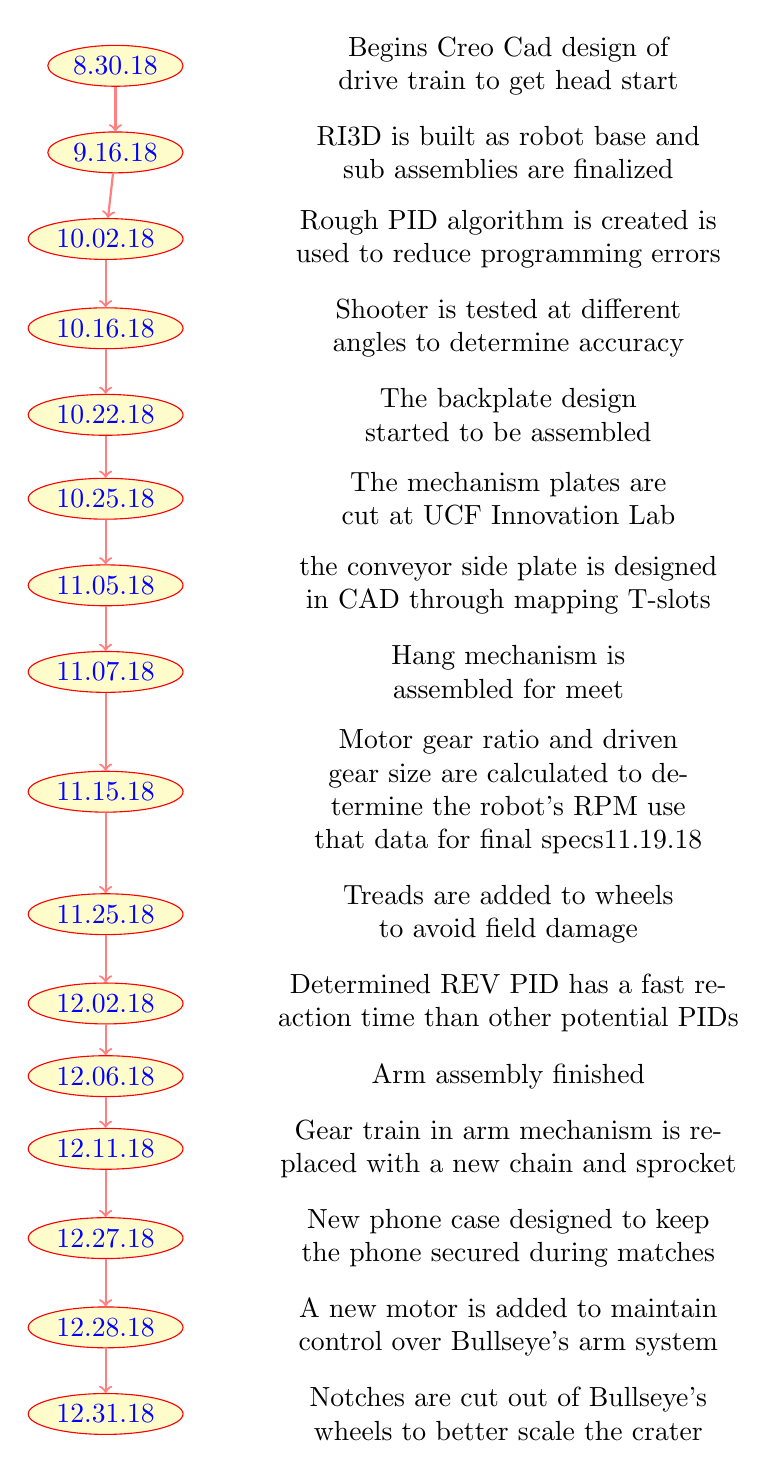
\begin{tikzpicture}[yscale=0.5,%
           year/.style={draw=red,text=blue,fill=yellow!20,shape=ellipse,inner sep=2pt},
           description/.style={rectangle,align=center,text width=60mm,anchor=west},
           timeline/.style={->,thick,red!50}]

    \foreach \year/\desc [count=\y] in {%
       8.30.18/Begins Creo Cad design of drive train to get  head start,
       9.16.18/RI3D is built as robot base and sub assemblies are finalized,%
       10.02.18/Rough PID algorithm is created is used to reduce programming errors,%
       10.16.18/Shooter is tested at different angles to determine accuracy,%
       10.22.18/The backplate design started to be assembled,%
       10.25.18/The mechanism plates are cut at UCF Innovation Lab,%
       11.05.18/the conveyor side plate is designed in CAD through mapping T-slots,%
       11.07.18/Hang mechanism is assembled for meet,%
       11.15.18/Motor gear ratio and driven gear size are calculated to determine the robot's RPM use that data for final specs%
       11.19.18/Big wheel drive train begans to go through design process,%
       11.25.18/Treads are added to wheels to avoid field damage,%
       12.02.18/Determined REV PID has a fast reaction time than other potential PIDs,%
       12.06.18/Arm assembly finished,%
       12.11.18/Gear train in arm mechanism is replaced with a new chain and sprocket,%
       12.27.18/New phone case designed to keep the phone secured during matches,%
       12.28.18/A new motor is added to maintain control over Bullseye’s arm system,%
       12.31.18/Notches are cut out of Bullseye’s wheels to better scale the crater%
       } { \ifnum\y=1 \node[description](\y){\desc};
           \else\node[description,below=1ex of \z](\y){\desc};
           \fi
           \node[year](y-\y) [left=of \y] {\year};
           \ifnum\y>1\draw[timeline] (y-\z)-- (y-\y);\fi
           \global\let\z=\y% for drawing from last node
       }




\end{tikzpicture}

\columnbreak

\raggedleft
\begin{center}
        \includegraphics[width=.13\textwidth]{Design_Overview/timephoto1.jpg}
\end{center}
\begin{center}
        \includegraphics[width=.13\textwidth]{Design_Overview/timephoto2.JPG}
\end{center}
\begin{center}
        \includegraphics[width=.13\textwidth]{Design_Overview/timephoto3.jpg}
\end{center}
\begin{center}
        \includegraphics[width=.13\textwidth]{Design_Overview/timephoto5.PNG}
\end{center}
\begin{center}
        \includegraphics[width=.13\textwidth]{Design_Overview/timephoto7.JPG}
\end{center}
\begin{center}
        \includegraphics[width=.13\textwidth]{Design_Overview/timephoto8.JPG}
\end{center}
\begin{center}
        \includegraphics[width=.13\textwidth]{Design_Overview/timephoto9.png}
\end{center}
\begin{center}
        \includegraphics[width=.13\textwidth]{Design_Overview/timephoto9-5.png}
\end{center}
\begin{center}
        \includegraphics[width=.13\textwidth]{Design_Overview/timephoto10.jpg}
\end{center}

\end{multicols}
\begin{multicols}{2}

\usetikzlibrary{shapes,positioning}

\newcommand{\foo}{\hspace{-2.3pt}$\bullet$ \hspace{5pt}}

\raggedright
\newcounter{year2}
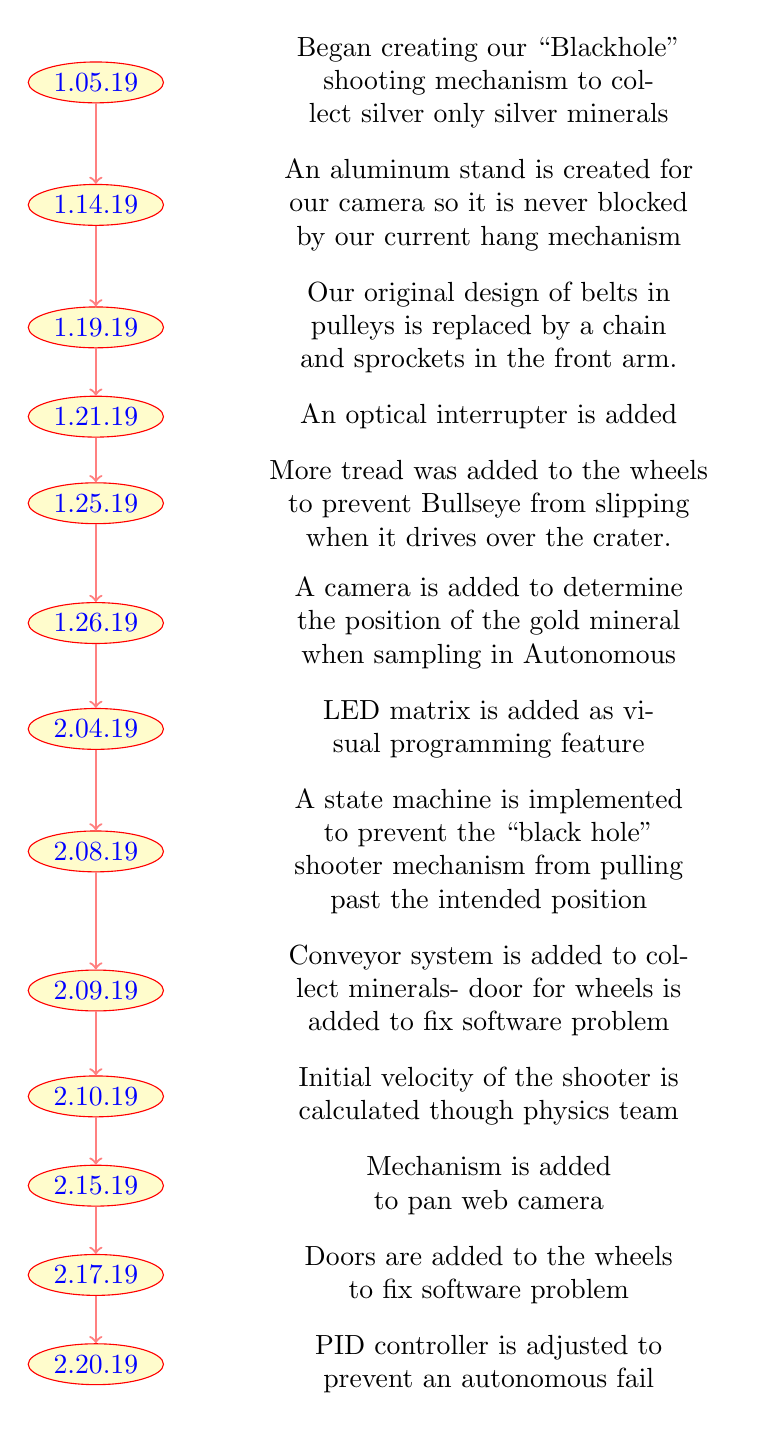
\begin{tikzpicture}[yscale=0.5,%
           year2/.style={draw=red,text=blue,fill=yellow!20,shape=ellipse,inner sep=2pt},
           description/.style={rectangle,align=center,text width=60mm,anchor=west},
           timeline/.style={->,thick,red!50}]

    \foreach \year/\desc [count=\y] in {%
       1.05.19/Began creating our “Blackhole” shooting mechanism to collect silver only silver minerals,%
       1.14.19/An aluminum stand is created for our camera so it is never blocked by our current hang mechanism,%
       1.19.19/Our original design of belts in pulleys is replaced by a chain and sprockets in the front arm.,%
       1.21.19/An optical interrupter is added,%
       1.25.19/More tread was added to the wheels to prevent Bullseye from slipping when it drives over the crater.,%
       1.26.19/A camera is added to determine the position of the gold mineral when sampling in Autonomous,%
       2.04.19/LED matrix is added as visual programming feature,%
       2.08.19/A state machine is implemented to prevent the “black hole” shooter mechanism from pulling past the intended position,%
       2.09.19/Conveyor system is added to collect minerals- door for wheels is added to fix software problem,%
       2.10.19/Initial velocity of the shooter is calculated though physics team,%
       2.15.19/Mechanism is added to pan web camera,%
       2.17.19/Doors are added to the wheels to fix software problem,%
       2.20.19/PID controller is adjusted to prevent an autonomous fail%
       } { \ifnum\y=1 \node[description](\y){\desc};
           \else\node[description,below=1ex of \z](\y){\desc};
           \fi
           \node[year2](y-\y) [left=of \y] {\year};
           \ifnum\y>1\draw[timeline] (y-\z)-- (y-\y);\fi
           \global\let\z=\y% for drawing from last node
       }


\end{tikzpicture}

\columnbreak

\raggedleft
\begin{center}
        \includegraphics[width=.13\textwidth]{Design_Overview/timephoto11.jpg}
\end{center}
\begin{center}
        \includegraphics[width=.13\textwidth]{Design_Overview/timephoto12.JPG}
\end{center}
\begin{center}
        \includegraphics[width=.13\textwidth]{Design_Overview/timephoto13.jpeg}
\end{center}
\begin{center}
        \includegraphics[width=.13\textwidth]{Design_Overview/timephoto14.jpg}
\end{center}
\begin{center}
        \includegraphics[width=.13\textwidth]{Design_Overview/timephoto15.png}
\end{center}
\begin{center}
        \includegraphics[width=.13\textwidth]{Design_Overview/timephoto16.png}
\end{center}
\begin{center}
        \includegraphics[width=.13\textwidth]{Design_Overview/timephoto17.png}
\end{center}
\begin{center}
        \includegraphics[width=.13\textwidth]{Design_Overview/timephoto18.jpg}
\end{center}
\begin{center}
        \includegraphics[width=.13\textwidth]{Design_Overview/timephoto19.png}
\end{center}


\end{multicols}
\clearpage
\addcontentsline{toc}{section}{\numberline{}Gamepad Controls}
\subsection*{\textbf{\Huge Gamepad Controls}}
\vspace{.2cm}
%\begin{flushleft}
\setlength{\parindent}{.25in} 
% guidelines http://www.firstinspires.org/sites/default/files/uploads/resource_library/ftc/2016-2017-season/engineering-notebook-guidelines.pdf
% starts at bottom of page 12

\textbf{Coach}: Ben Steinebronn \\
\textbf {Driver 1}: Shey Naik \\
\textbf {Backup}:	Jonathan Valentin \\
\begin{figure}[h!]
\centering
\includegraphics[width=0.65\textwidth, angle=0]{Design_Overview/DriverController.png}
\caption{Driver - Gamepad 1 Controls}
\label{fig:Gamepad1}
\end{figure}

\clearpage

\textbf{Driver 2}: Jolie Miller \\
\indent \textbf{Backup}: Austin English \\
\begin{figure}[h!]
\centering
\includegraphics[width=0.65\textwidth, angle=0]{Design_Overview/OperatorController.png}
\caption{Operator - Gamepad 2 Controls}
\label{fig:Gamepad2}
\end{figure}

\insertdesignoverview{Drivetrain}
{Create a stable drivetrain that can scale the crater to recover minerals quickly and effectively} % Goals of the mechanism
{10-12.JPG}% CAD Image
{drivetrain_1.JPG}% Build Image
{0.25" Medium Density Fiberboard, Aluminum, ABS Plastic, Steel, Retaining Rings}% Materials ex. 0.25" MDF, Aluminum, etc
{Laser Cutting, 3D Printing, CNC Milling, Lathe}% Manufacturing Processes ex. Laser Cut, 3D print, etc.

\subsection*{How it Works}
The drivetrain is composed of two modules connected by a center chassis where the motors are built on. Each module has two 20:1 BaneBots planetary gearboxes which spin a driver gear. This gear is meshed in a 1:4 ratio to the gear attached to each wheel. Each 16" wheel has a notch cut in it to allow us to go over the crater. The wheel assemblies ride on bearings that are fixed onto custom 3D printed pieces in the wood.

\begin{figure}[htp]
\centering
\includegraphics[width=.8\linewidth]{Design_Overview/DT_cad.PNG}
\caption{Another look at the CAD of our Drivetrain}
\label{fig:iteration}
\end{figure}

\subsection*{Iterations}
In prior years, our team utilized belts and pulleys to power our drive train. We found that for this game, going over the crater is essential and bigger wheels would make that task much easier than having a low profile drive train with belts and pulleys. Our first prototype consisted of four 40:1 motors with a 40T driver gear actuating a 120T gear on the output shaft. However, given that the stabilization arms required another two motors, we tried something new by only using one motor to power each side. This worked fairly well for the team, as we didn't compromise on speed or efficiency. In addition, we had to make some changes to provide some horizontal support. 

\subsection*{Mechanism Accomplishments}
\begin{itemize}
    \item It can drive up the crater
    \item It can quickly traverse the field, going from the crater to the lander
    \item Its design allows for more space to add more components
\end{itemize} 


\insertdesignoverview{Chassis Stabilization Arms}
{Stabilize the chassis and set to numerous positions for various teleop objectives} % Goals of the mechanism
{arms_CAD.PNG}% CAD Image
{arms_build.PNG}% Build Image
{.25" Medium Density Fiberboard, Aluminum Shafting, PLA Plastic, Steel 1/2" Radial Bearings}% Materials ex. 0.25" MDF, Aluminum, etc
{Laser Cutting, 3D Printing, Lathe work, CNC Milling}% Manufacturing Processes ex. Laser Cut, 3D print, etc.


\interesting{Accomplishing chassis stabilization through innovative arms}{Innovate:55}
\interesting{}{Stabilize:1}

\subsection*{How it Works}
40:1 Torquenado motors actuate the arms using chain and sprocket with a 1:2 gear ratio. Each side features two 8" arms with skateboard wheels. Zeroed perpendicular to the chassis, the arms set to a natural stabilization position during autonomous, keeping Bullseye's floating chassis level as it drives. During crater scaling, the arms are programmed to actuate in accordance with the gyroscope, moving to keep the chassis balanced. Another arm set position readies the robot for shooting. Photointerruptors on each side ensure that the arms can find it's position during teleop in case of emergency.   

\subsection*{Modelling \& Simulation}
When designing the chassis stabilization arms, we established a body skeleton of the robot in PTC Creo, which was a basic sketch of the whole robot with set axes and coordinate systems. Then, we created motion skeletons for the individual arms. From there, we could build our parts around the skeleton, and attach them to the moving bodies. We could then simulate the movement within the motion skeleton. These skeletons not only helped us define the geometry and joints of the arms with several sketches, but they made major part modification simple since they're referenced to a base sketch, thus allowing us to change the arm design with ease. 

\begin{figure}[h!]
\centering
\begin{minipage}{.48\textwidth}
  \centering
  \includegraphics[width= .8\linewidth]{Design_Overview/Stabilization_Skeleton.PNG}
\end{minipage}%
\hfill
\begin{minipage}{.48\textwidth}
  \centering
  \includegraphics[width= .8\linewidth]{Design_Overview/Skel.PNG}
\end{minipage}
\end{figure}


\subsection*{Iterations}
Originally, our prototype chassis stabilization was done with primitive integration of the 4" Tetrix Omni Wheels and a short arm length. Not only did this haphazardous assembly fail to integrate well, with several wood spacers used to distance the bronze bushing to install the wheels, but the skinny wheel also made travel on the tiles much more difficult. We replaced the omnis with skateboard wheels, which made integration simple as it only required an 8mm screw with a washer and a nut. Another significant iteration we made was in regards to the arms' actuation. At first, we'd used HTD belts and 3D printed nylon pulleys with the same 1:2 ratio, yet we quickly recognized that the belt required incredible tension to run smoothly without skipping, which was so strong that it would twist the motor out of place, causing the belt to be loose yet again and causing it to skip. Realizing that a chain and sprocket system would be much more robust and less vulnerable to skipping, we replaced our pulleys with 16T to 32T VexPro sprockets with chain. 

\interesting{Design Iteration of the Stabilization Arms, Mark I to Mark V}{Design:4}

\begin{figure}[h!]
\centering
\includegraphics[width=.8\linewidth]{Design_Overview/Iteration.jpg}
\caption{Design Iteration of the Stabilization Arms, Mark I to IV}
\label{fig:iteration}
\end{figure}

\begin{figure}[h!]
\centering
\begin{minipage}{.32\textwidth}
  \centering
  \includegraphics[width= .9\linewidth]{Design_Overview/front_arm.JPG}
\end{minipage}%
\hfill
\begin{minipage}{.32\textwidth}
  \centering
  \includegraphics[width= .9\linewidth]{Design_Overview/both_arms.JPG}
	\caption{Final Stabilization Arms, Mark V}
	\label{fig:Triple_Arm_IMG}
\end{minipage}%
	\hfill
\begin{minipage}{.32\textwidth}
  \centering
  \includegraphics[width= .9\linewidth]{Design_Overview/rear_arm.JPG}
\end{minipage}
\end{figure}

\subsection*{Sensors and Control}
Two photointerruptors, one on each side, are used for emergency recalibration of the arms at their natural position. Two laser cut wooden flanges on each arm break the light beam of the photointerruptor, setting a known position for the arm. However, understanding that the encoders aren't perfect, and given the backlash of the chain, we understood that we had to come back up and return slower in order to calibrate at exactly the right position for driving smoothly. In addition, we use the internal PID on the REV Expansion Hub for stabilization, and utilize preestablished angles for various telemetry operations, such as intaking minerals, shooting into the lander, or hanging on the latch. For determining level driving angles for the arms, our physics division determined a formula to calculate the angle at which one arm would have to be in relation to the other. 

%\begin{figure}[h!]
%\centering
%\begin{minipage}{.48\textwidth}
%  \centering
%  \includegraphics[width= .8\linewidth, angle=-90]{Meetings/January/01-21-19/interrupter.png}
%\end{minipage}%
%\hfill
%\begin{minipage}{.48\textwidth}
 % \centering
%  \includegraphics[width= .75\linewidth, angle=-90]{Design_Overview/photo_int_real.JPG}
%\end{minipage}
%\end{figure}

\vskip 0.35in
\textbf{Different Arm Preset Positions:}
\textit{Various Preset Positions for the Stabilizing Arms}

\interesting{Various Preset Positions for the Arms}{control:3}

\begin{figure}[h!]
\centering
\begin{minipage}{.32\textwidth}
  \centering
  \includegraphics[width= .9\linewidth]{Design_Overview/Zero.JPG} %%zero
\end{minipage}%
\hfill
\begin{minipage}{.32\textwidth}
  \centering
  \includegraphics[width= .9\linewidth]{Design_Overview/45.JPG} %%45
\end{minipage}%
  \hfill
\begin{minipage}{.32\textwidth}
  \centering
  \includegraphics[width= .9\linewidth]{Design_Overview/90.JPG} %%90
\end{minipage}
\end{figure}

\begin{figure}[h!]
\centering
\begin{minipage}{.32\textwidth}
  \centering
  \includegraphics[width= .9\linewidth]{Design_Overview/Natural.JPG} %%natural
\end{minipage}%
\hfill
\begin{minipage}{.32\textwidth}
  \centering
  \includegraphics[width= .9\linewidth]{Design_Overview/hang_angle.JPG} %%shooting
\end{minipage}%
  \hfill
\begin{minipage}{.32\textwidth}
  \centering
  \includegraphics[width= .9\linewidth]{Design_Overview/shooter_angle.JPG} %%hang
\end{minipage}
\end{figure}

\vskip 0.25in
Chassis Stabilization and Level Driving Angles: 
\vskip 0.05in
\textit{
\\The goal is to maintain ground contact of both stabilization arms in order to drive smoothly. 
}

\vskip 0.2in
\begin{equation}
\phi_{front} = \arccos(\frac{sin(\theta) + 6.7 + 6.5}{8.0} - 90 + \theta)
\end{equation}

\begin{equation}
\phi_{back} = \arccos(\frac{-sin(\theta) + 6.7 + 6.5}{8.0} + 90 + \theta)
\end{equation}

\subsection*{Equation Analysis}
\textit{
\\ With the use of one of the angles, we can calculate the angle of the other arm to be stable; Refer to the January 20th entry to learn more about how these equations work, and how we created them. 
}

\interesting{Writing Formulas for Arm Stabilization}{control:2}

\subsection*{Mechanism Accomplishments}
\begin{itemize}
    \item Uniformly stabilize the chassis, maintain ground contact to ensure smooth driving
    \item Set to the prepositioned intake angle to pick up minerals
    \item Set to the prepositioned shooter angle for mineral deposit 
    \item Set to the prepositioned hang angles for the endgame in TeleOp
\end{itemize} 
\insertdesignoverview{Hang Winch}
{Create a fast, reliable hang mechanism to latch and de-latch in both autonomous and endgame} % Goals of the mechanism
{Hang.PNG}% CAD Image
{fullbullseyehang.PNG}% Build Image
{Steel rods, Duracord, Surgical Tubing, Aluminum}% Materials ex. 0.25" MDF, Aluminum, etc
{Laser Cutting, CNC Milling, Metal Bending}% Manufacturing Processes ex. Laser Cut, 3D print, etc.

%\interesting{Our innovative glyph delivery mechanism, analyzed in depth}{Innovate:55}

\subsection*{How it Works}
The hang mechanism works by attaching a hook onto the end of the front arm. This hook has a winch connected to it that runs through the robot and to the underside where a 40:1 motor turns, lifting the robot. The claw gets to the latch by tilting the robot so that the front arm sticks up in the air. The claw than rotates due to a small servo on the arm to put the hook into the latch when the winch motor pulls the robot up. In autonomous, the winch motor spins the opposite way to lower the robot and unhooks by tilting the robot to push up. 

 \begin{figure}[h!]
 \centering
   \includegraphics[width=0.8\textwidth, angle=0]{Design_Overview/Hang_1.PNG}
  \caption{Hang Top Pic}
  \label{fig:hang_top}
 \end{figure}

\subsection*{Modelling \& Simulation}
Modelling the hang mechanism involved minimal design challenges. The only thing we originally struggled with was how the arms would line up with the lander. In order to model this, we used body and motion skeletons to see the distance to the latch as well as how far in it would reach. However, issues were primarily resolved through design iteration, as you'll see below. 

\subsection*{Iteration}
Initially,we angled the hang plate that held the hook, believing that that would allow for the hook to be well within the latch. However, after testing, we determined that a straight hang plate worked much better. We also made several iterations of a winch box that would rest at the back of the chassis, yet after struggling with space issues we realized that we could simply mount the motor directly on the underbelly of the chassis with a hole to guide the winch string.

\begin{figure}[htp]
\centering
\includegraphics[width=.8\linewidth]{Design_Overview/Hang_Iteration.jpg}
\caption{Design Iteration of the Hang, Mark I to Mark IV}
\label{fig:hang_iteration}
\end{figure}

\begin{figure}[htp]
\centering
\begin{minipage}{.32\textwidth}
  \centering
  \includegraphics[width= .9\linewidth]{Design_Overview/Hang_Left.JPG}
\end{minipage}%
\hfill
\begin{minipage}{.32\textwidth}
  \centering
  \includegraphics[width= .9\linewidth]{Design_Overview/Hang_Front.JPG}
	\caption{Final Hang Mechanism, Mark V}
	\label{fig:hang_final_IMG}
\end{minipage}%
	\hfill
\begin{minipage}{.32\textwidth}
  \centering
  \includegraphics[width= .9\linewidth]{Design_Overview/Hang_Right.JPG}
\end{minipage}
\end{figure}

\subsection*{Sensors and Control}
The winch motor uses encoder PID to hold the hang position during autonomous. In addition, we use two buttons for autonomous setup, with the buttons controlling winching up or winching down. Wanting to determine the power of the motor, our physics team developed a formula to determine the amount of torque that the motor needs to pull the horn down. These equations are described below. 

\insertdesignoverview{Intake Mechanism}
{Pick up one piece of freight quickly and easily, hold the freight securely as the arm pivots upwards to the back of the robot, and outtake the freight at any level one either of the shipping hubs. Ensure that the freight can be picked up in autonomous as well as tele-op.
} % Goals of the mechanism
{intake_CAD.PNG}% CAD Image
{intake_build.JPG}% Build Image
{1/8” Birch Plywood, 1.5 mm Fiberglass Plate, Nylon Plastic, Rubber Sheet}% Materials ex. 0.25" MDF, Aluminum, etc
{Laser Cutting, 3D Printing, Cutting on Bandsaw}% Manufacturing Processes ex. Laser Cut, 3D print, etc.
\subsection*{How it Works}
Our intake uses a fast-moving sweeper with two rubber flaps which spin and pull freight into our intake. The sweeper is driven by a GoBilda super speed servo through three stages of belts and pulleys. The third stage of the belt, which has the primary function of transferring rotation to the sweeper, is located in the middle of the intake, allowing it to function as a conveyor belt to pull the freight all the way in. To ensure that we could intake the different sized blocks and balls while maintaining a tight enough grip on whichever one we have, the final stage of our intake, where the sweeper is attached, can pivot. Aided by rubberbands which tension the pivoting stage downwards, the sweeper can adapt to the size of whichever element is being collected.  To limit unnecessary complication in our design, our intake is pivoted up and back to the right height of whichever hub we plan to score in and can outtake the freight it was carrying. By simply reversing the sweeper, we can push the freight being carried out of the robot and into a hub.



% \begin{figure}[h!]
% \centering
% \includegraphics[width=0.8\textwidth]{Design_Overview/exploded_intake.PNG}
% \caption{Exploded View of the Intake Mechanism}
% \label{fig:exploded_intake}
% \end{figure}

% \begin{figure}[h!]
% \centering
% \includegraphics[width=0.8\textwidth]{Design_Overview/Sorting.JPG}
% \caption{Passive Sorting}
% \label{fig:sorting}
% \end{figure}

% \subsection*{Modelling \& Simulation}
% Much like all of our other mechanisms, we designed and simulated the intake using body and motion skeletons in PTC Creo. The most challenging issue with designing the intake was determining how far forward the rubberband wheels would be, as well as the size of the wheel itself. To make this easier on ourselves, we created sketches of the silver and gold minerals in the body skeleton and referenced it to design a smooth curve upwards that would maintain contact with the intake wheel. \hl{Our use of skeletons makes part implementation simple and fast, and facilitated continuous design iteration.} See below in Figures \ref{fig:skel_intake} and \ref{fig:skel_intake_use} to see how we implemented skeletons into our design. 

%    \begin{figure}[ht!]
% 	\centering
% 	\begin{minipage}{.48\textwidth}
% 	  \centering
% 	  \includegraphics[width=0.8\linewidth]{Design_Overview/skel_intake.PNG}
% 	  \caption{The Intake Arm and Minerals in the Body Skeleton}
% 	  \label{fig:skel_intake}
% 	\end{minipage}%
% 	\begin{minipage}{.48\textwidth}
% 	  \centering
% 	  \includegraphics[width=0.8\linewidth]{Design_Overview/skel_intake_in_use.PNG}
% 	  \caption{The Skeleton in Use with Intake}
% 	  \label{fig:skel_intake_use}
% 	\end{minipage}
% 	\end{figure}

% \subsection*{The Phillip Mech}
% At the back of the intake, we have a mechanism to transfer the silver into the shooter (something our team refers to as Phillip). This consits of a REV servo that flips up. The arm is made of laser cut mdf made to have specially bent piano wire that works by having the intake bend the piano wire slightly out to get the silver in and then bends back to normal when the silver gets all the way in. The reason we use piano wire is that it holds its shape really well which means that it is hard to bend permanently but is easy to flex outward to allow for the silver to fall into the tray that goes up to the shooter.

%    \begin{figure}[ht!]
% 	\centering
% 	\begin{minipage}{.48\textwidth}
% 	  \centering
% 	  \includegraphics[width=0.8\linewidth]{Design_Overview/Phillip_1.JPG}
% 	  \caption{Loading The Transfer Mechanism}
% 	\end{minipage}%
% 	\begin{minipage}{.48\textwidth}
% 	  \centering
% 	  \includegraphics[width=0.8\linewidth]{Design_Overview/Phillip_2.JPG}
% 	  \caption{Transfer Mechanism Deposit to the Shooter}
% 	\end{minipage}
% 	\end{figure}

\subsection*{Iterations}
Initially, we built our intake to utilize a grabbing mechanism rather than a sweeper. Although our grabber became quite effective after making several tweaks to its design, we felt that we had hit a ceiling for its efficiency. Additionally, it is much harder to pick up freight in autonomous with a grabbing mechanism compared to with a spinner intake. Seeing this, we tested with a couple of types of spinners, including a roller wrapped in surgical tubing, and found the sweeper design to be most effective. 


% PUT THIS PHTOTO HERE: Design_Intake_Image3

One of the early designs of a spinner intake that we made had the sweeper positioned at a fixed height. We quickly found that this limited us to only being able to reliable hold the blocks which are smaller than the wiffle balls. When we tried to increase the height of the sweeper to allow us to intake the balls, we found that the blocks would slip out of the intake as we pivoted the arm, sometimes launching the block and incurring penalties. Observing this, we created our pivoting sweeper which can much more effectively grab and hold freight of different sizes.

% PUT THIS PHTOTO HERE: Design_Intake_Image4

Another thing we learned from a previous spinner intake design was the effectiveness of different materials on the sweeper. We initially started testing with surgical tubing, a popular material for FTC intakes but found that it didn’t live up to the utility we had expected seeing so many teams use a similar design. Instead, we tried several different materials and designs that we came up with ourselves and found many of them to be much more successful than the surgical tubing. Ranging from zip ties to different types of foam, we tested many materials and forms, eventually finding rubber strips we had cut from a sheet of rubber to be most effective. To increase the effectiveness of the rubber flaps, we laser cut them to get a cleaner and more precise shape.


% \interesting{Iterative Design with the Intake}{design:6}

% \begin{figure}[htp]
% \centering
% \includegraphics[width=.8\linewidth]{Design_Overview/Intake_Iteration.jpg}
% \caption{Design Iteration of the Intake, Mark I to IV}
% \label{fig:intake_it}
% \end{figure}

% \begin{figure}[htp]
% \centering
% \begin{minipage}{.32\textwidth}
%   \centering
%   \includegraphics[width= .9\linewidth]{Design_Overview/Intake_Left.JPG}
% \end{minipage}%
% \hfill
% \begin{minipage}{.32\textwidth}
%   \centering
%   \includegraphics[width= .9\linewidth]{Design_Overview/Intake_Front.JPG}
% 	\caption{Final Intake, Mark V}
% 	\label{fig:triple_intake_IMG}
% \end{minipage}%
% 	\hfill
% \begin{minipage}{.32\textwidth}
%   \centering
%   \includegraphics[width= .9\linewidth]{Design_Overview/Intake_Right.JPG}
% \end{minipage}
% \end{figure}

\subsection*{Sensors and Control}
We have one color sensor attached to the top of our intake to allow us to sense if we have grabbed a block during the autonomous period. This allows the robot to know when it should leave the warehouse to score the freight it has collected. It is also used to automatically raise the arm so we can get rid of any extraneous freight. 

\subsection*{Mechanism Accomplishments}
\begin{itemize}
    \item Allow for autonomous pick up
    \item Lightweight to reduce motor stress
    \item Firm block grip 
    \item Adapts to any size freight
\end{itemize} 
\insertdesignoverview{The Black Hole Shooter}
{Shoot quickly and efficiently into the lander} % Goals of the mechanism
{Shooter_CAD.PNG}% CAD Image
{Shooter_Parts.JPG}% Build Image
{Elastic Sheet (25\% Spandex and 75\% Nylon), quarter inch MDF, lexan, one way bearing, steel ball, aluminum}% Materials ex. 0.25" MDF, Aluminum, etc
{Laser Cutting, 3D Printing, CNC Routing}% Manufacturing Processes ex. Laser Cut, 3D print, etc.

%\interesting{Our innovative glyph delivery mechanism, analyzed in depth}{Innovate:55}

\subsection*{How it Works}
 A ring is cut from MDF in an oval shape with a closely fitting larger ring. The larger ring is not continuous and aluminum material is screwed onto it to allow tightening. The elastic sheet is placed, taut, over the inner ring and under the larger ring. The larger ring is then tightened to secure the sheet. The steel ball is then placed in the center of the sheet and tied into the sheet on the underside. On the shaft of a REV core hex motor is a lever cut from lexan with a one way bearing secured within it. The lexan lever is then tied to the steel ball on the underside. The REV core hex motor rotates a 1.5 inch lexan lever down. When the lever rotates past 180 degrees, the one way bearing is allowed to freely move back to the original position. The lexan lever is tied to the elastic sheet and is pulled down up to 3 inches when it is rotated. 

\subsection*{Modelling \& Simulation}


\subsection*{Iteration}
The lever was initially made of quarter inch MDF which snapped due to the vertical force on the lever. The lever was also extended longer than it needed to be initially. The ring initially did not have a tightening ring around it, instead the sheet was tied to the ring.


\begin{figure}[htp]
\centering
\includegraphics[width=.8\linewidth]{Design_Overview/Shooter_Iteration.JPG}
\caption{Design Iteration of the Shooter, Mark I and Mark II}
\label{fig:iteration}
\end{figure}

\begin{figure}[htp]
\centering
\begin{minipage}{.32\textwidth}
  \centering
  \includegraphics[width= .9\linewidth]{Design_Overview/Shooter_Left.JPG}
\end{minipage}%
\hfill
\begin{minipage}{.32\textwidth}
  \centering
  \includegraphics[width= .9\linewidth]{Design_Overview/Shooter_Front.JPG}
  \caption{Final Stabilization Arms, Mark III}
  \label{fig:Triple_Arm_IMG}
\end{minipage}%
  \hfill
\begin{minipage}{.32\textwidth}
  \centering
  \includegraphics[width= .9\linewidth, angle=180]{Design_Overview/Shooter_Right.JPG}
\end{minipage}
\end{figure}

\subsection*{Sensors and Control}
An equation was made by the physics team to describe the peak vertical force on the system. Another equation was made to calculate the torque as the lever goes around. This is to ensure that the material and structure of the lever made will be able to support the tension from the sheet. Refer to the engineering section to find the formulas we calculated and used. 
\cleardoublepage


 %            _____                           _   _ _   _               _____           _            
 %           / ____|                         | | (_) | (_)             |  __ \         | |           
 %  ______  | |     ___  _ __ ___  _ __   ___| |_ _| |_ _  ___  _ __   | |__) |_ _ _ __| |_   ______ 
 % |______| | |    / _ \| '_ ` _ \| '_ \ / _ \ __| | __| |/ _ \| '_ \  |  ___/ _` | '__| __| |______|
 %          | |___| (_) | | | | | | |_) |  __/ |_| | |_| | (_) | | | | | |  | (_| | |  | |_          
 %           \_____\___/|_| |_| |_| .__/ \___|\__|_|\__|_|\___/|_| |_| |_|   \__,_|_|   \__|         
 %                                | |                                                                
 %                                |_|    

\part{Competition Section}
\begin{minipage}[c]{\linewidth}
\centering
\includegraphics[width=\linewidth]{Images/Main/competitionwoo.jpg}
\end{minipage}

\insertCompetition
{Ruckus at the Rock}
{02/02/2019}
{Hagerty High School}
{5th}
{driveteam.jpg}
{driveteam.jpg}
{driveteam.jpg}
{\lipsum{1}}

% \addcontentsline{toc}{chapter}{\numberline{}Lessons Learned}
\subsection*{\textbf{\Huge Lessons Learned:}}
\vspace{.2cm}
%\begin{flushleft}
\setlength{\parindent}{.25in} 
\interesting{   }{LessonsLearned:1}
Every season, we as the Mechromancers regard our competitions as being \hl{less about winning or losing}, and more as a learning experience, with \hl{every success and failure acting as a lesson}, providing the bright minds on our team with real engineering insight into what works and what doesn't. The Mechromancers realize the significance of the process of trial and error in the engineering and design process, and understand how much it contributes to \hl{encouraging creative thinking and innovation within the team}. For this reason, we have always recorded our results in meets and competitions, and present what we learned on competition day in a small, bulleted section called "lessons learned" within each competition entry. The Relic Recovery season featured an abundance of adaptation and change through experience for the Mechromancers. Here, you can learn about the \hl{difficulties we faced as a team within each competition, how we overcame these difficulties through design changes and new innovations, and the reasoning behind each new iteration of Buzz} that the Mechromancers conjured over the season. 
\begin{figure}
 \centering
 \begin{minipage}{.48\textwidth}
   \centering
   \includegraphics[width=\linewidth]{Competition/Old.JPG}
   \caption{The Mechromancers' First Iteration of Buzz}
   \label{fig:FirstIt}
 \end{minipage}%
\hfill
 \begin{minipage}{.48\textwidth}
   \centering
   \includegraphics[width=\linewidth]{Competition/New.PNG}
   \caption{Buzz after the Season's Evolutions}
   \label{fig:Evolved}
 \end{minipage}
 \end{figure}
The first permutation of Buzz holds almost no resemblance to the Buzz that the world knows today, and only goes to show how the team adapts to challenges and adversity. Before our very first meet of the season on November 11th, the Mechromancers planned to design a robot with \hl{simplicity, speed and modularity in mind} that could easily pick up glyphs and score them within the cryptobox, and could \hl{possibly be automated easily for multiple glyph delivery}. We designed a fast and modular drivetrain, with our intake mechanism attached to two sliding rails, supplementing an elevator system. This elevator, consisting of a 20:1 motor powering a series of pulleys that pulled the intake mechanism up and down, allowed a simple method of glyph delivery that featured the glyphs to be intaked and delivered using the same mechanism. Although simplistic in design, this permutation of Buzz featured several design flaws that inhibited efficient glyph delivery. For example, one issue that the team struggled with frequently shortly before our first competition was how \hl{the force of gravity counteracted the lifting of the elevator mechanism}, as for the elevator to remain at a set position, it required power to be supplied constantly and at a greater rate. At one point, this even led to our pulley motor browning out. We also noticed that the glyphs, once pulled into our intake, remained close together and made glyph delivery difficult, often causing glyphs to descore and fall out of the column. Another issue that we noticed with this iteration of Buzz was the \hl{lack of control} it offered. The robot's simplistic design inhibited the calculated manipulation of glyph delivery, or the lack of a chance to improve efficiency through autonomy. Recognizing the significance of these design flaws through our experiences leading up to and on competition day, the Mechromancers \hl{took these valuable lessons in consideration when designing a new glyph delivery mechanism that took advantage of the force of gravity in its glyph scoring, and featured more of an ability to control and manipulate the mechanism as well}, not only enabling better driver operated performance, but permitting further advancements in the autonomous period (such as our goal to score multiple glyphs in autonomous). 
  \begin{figure}[htp]
  \centering
    \includegraphics[width=\textwidth, angle=0]{Competition/Old2.JPG}
   \caption{Buzz at our First Meet on November 11th}
   \label{fig:Nov11}
  \end{figure}
The second version of Buzz, prevailing at our second meet of the season on December 9th, solved such design flaws magnificently. Not only did \hl{the arms take advantage of gravity, delivering glyphs at the back of the robot and allowing them to slide down} into the cryptobox columns, but they provided an increased ability to use sensors and algorithms to refine TeleOp and Autonomous performance. The sliders on \hl{the arms could be preprogrammed, the claws could be automated, and almost all aspects of glyph delivery could be done without driver control.} Best of all, it was a \hl{unique and innovative} method that was unparalleled to our competition. However, this didn't mean that we didn't face issues at the second meet. The glyph separation mechanism of using two belts to pull the glyphs apart malfunctioned frequently, and our glyph delivery was often slowed due to the precarious aligning required during delivery. Yet again, through what we'd learned on the competition field, we continued to innovate and make improvements, getting ready for League Championships. Now, the team began to \hl{fully utilize our sensors and algorithms to automate glyph delivery positions, the glyph pickup position, and the sychronization of both arms.} We also used a \hl{multitude of cameras to give Buzz vision, continuing to perfect the autonomous and working to complete the jewel hitter.} The amalgamation of the hardware of our robot with the software was what finally gave Buzz life. And although Buzz has already served the Mechromancers most of the entire season, the team agrees that the robot is nowhere close to finished, as the Mechromancers \hl{forever continue to innovate and improve.} 
  \begin{figure}[htp]
  \centering
    \includegraphics[width=\textwidth, angle=0]{Competition/New2.JPG}
   \caption{Buzz, New and Improved}
   \label{fig:NewBuzz}
  \end{figure}
  On the following pages, you'll find our competition entries throughout the season, with a description of what happened at each event as well as all of the lessons we learned through our performance on competition day. This is followed by our "lessons learned" subsection, as well as a match results table depicting our overall performance through our statistics on the field. 
% \insertcompetition{11/10/18} {Ruckus at the Rock}{match.jpg}{driveteam.jpg}{16th} 
{

	\bigskip

	\textbf{Robot:}  Our hanging mechanism may have been slightly too ambitious for our first meet, because even though it was elegant and innovative, we were unable to make it work for the competition. We also focused too much of our time on the hanging mechanism, so we had a very basic collection mechanism that could only deposit in the depot. We had some minor success after taking off the hanging mechanism, which made our robot short enough to fit under the lander and much faster. This taught us that sometimes it is a good strategy to remove parts of the robot that are nonfunctional if it provides some other advantage, and it may be a good strategy to make our robot shorter so it can more easily navigate the field.

	\bigskip

	\textbf{Competition:} We need a more detailed checklist and more focus on packing. We forgot many integral things which made the competition more difficult and more stressful than it should have been, including the team marker and controller board. We made a list of things we forgot to improve our packing checklist and ensure that next time we double check that everything on the list is packed. Our scouting team was successful in gathering valuable information about the other teams, so we will continue with that method, most likely with newer members so they can learn how to do it. 

	\bigskip

	\textbf{General:} We need a more detailed schedule for when we want to achieve our goals, especially for when we want to complete certain parts of the robot. While we did plan to finish things far enough in advance to build in time for programming and driver practice, we ultimately did not achieve these goals and left ourselves with too little time to achieve as much as we had hoped to for the competition.

	\bigskip

	\textbf{Goals for Upcoming Qualifiers:} Finish building it at least 2 weeks before the competition so that it can be programmed and the drivers can have time to practice.

	\bigskip

	\textbf{Administrative:} Because of the issues we faced with completing the necessary work by the intended time, we will be using Trello, our project management app, to a larger extent. This means members will need to claim a task on Trello at the beginning of each meeting, ensuring everyone is working. Also, goals for when tasks should be finished will be put on both Trello and Band to hold people accountable to their goals.

	\bigskip

	\textbf{Robot:} We need to redesign our hanging mechanism to be stronger, easier to use, and more reliable, which will likely require a total change in concept. We also need a more effective method for collecting and scoring minerals into the lander. We are currently considering using an arm to extend into the crater to save time, but need to consider different methods of collection, such as rubber bands or surgical tubing. Finally, we must decide if we want to reach into the crater with an arm or drive in. If we are driving in, we need a new drivetrain, as our current one had trouble getting over the crater wall.

	\bigskip

	\textbf{Long-term Goals:} We must win 8 matches in our next 2 competitions to remain competitively viable in the League Championship, which increase our chances of moving on to States.

	\bigskip

	Unfortunately we didn’t perform as well as we had hoped to at our first meet. Our hang mechanism broke after practicing hanging off of the playing field and we had multiple problems with our code. We finished the day 16th with 2 wins and 4 losses. While we had many issues day of the competition, this was a great learning opportunity for everyone on our team. We plan to work on our time management and improving our designs with more prototyping and testing.
}
{
  \begin{itemize}
      \item Test software changes multiple times before matches; don't make sudden changes to the program before a match without testing
      \item Leave a full week after hardware and software changes for realistic and thorough driver practice to prepare drivers completely for the competition
      \item Practice the transition between the autonomous and teleop period 
      \item Keep multiple RC and DS phones fully charged for the day of the competition
      \item Keep some essential tools from the pits in a portable case along with the pits checklist 
  \end{itemize} 
}
{Rockledge High School, Rockledge, Fl}
\begin{figure}[ht]
  \centering
  \includegraphics[width=0.9\textwidth]{Competition/Images/Meet1Score.PNG}
  \caption{}
  \label{fig:comparinggears}
\end{figure} 
\interesting{Our first meet at Rockledge High School}{competition:1}
% \include{Competition/Meet2_LessonsLearned}
% \include{Competition/Meet3_LessonsLearned}
% \include{Competition/LeagueChamps}
\cleardoublepage
%\partimage[width=1.1\textwidth]{Images/Main/cover.png}
\appendix
%\appendixpage

%\chapterstyle{plain}
%\pagestyle{hhs_ruled}
%\aliaspagestyle{chapter}{plain}
\section{Custom Parts Reference}

\newcommand{\referencehelper}[2]{
 \begin{figure}[ht!]
 \centering
   \includegraphics[width=\textwidth, angle=0]{CAD/#1.pdf}
  \caption{#2}
 \end{figure}
}

\interesting{  }{CustomPartsReference:1}
\referencehelper{big_wheel_hub}{Big Wheel Hub}


%\chapterstyle{southall}
\listoffigures
%\end{flushleft}

\end{document}
